\documentclass[12pt,a4paper]{article}
 
\usepackage{float}
%für feststellen der figures und tables [H] dranschreiben
\usepackage{units}
%wird so benutzt: 
%\unit[value/Zahl]{dimension/Einheit} oder 
%\unitfrac[value/Zahl]{dimension/Einheit num/Zähler}{dimension/Einheit denum/Nenner} oder
%\nicefrac[fontcommand/Schriftart]{dimension/Einheit num/Zähler}{dimension/Einheit denum/Nenner}

\usepackage{caption}
\usepackage{subcaption}

\usepackage[left=2cm,right=2cm,top=2cm,bottom=2cm]{geometry}
\usepackage[utf8]{inputenc}
\usepackage[T1]{fontenc}
\usepackage{lmodern}
\usepackage[ngerman]{babel}
\usepackage{amsmath}
\usepackage{graphicx}
 
\title{Versuch EP2 Die Diode}
\author{Frederik Strothmann, Henrik Jürgens}
\date{\today}
%niemals zwei überschriften direkt übereinander schreiben, also immer mindestens in einem satz was sinnvolles unter jede überschrift schreiben (bei den versuchen z.B. das versuchsziel) 
\begin{document}
%deckblatt erstellen.
\maketitle
\newpage
\tableofcontents
\newpage
\section{Einleitung}
%einleitung zu dem experiment.
%auf die einstellungen, die vor dem versuch gemacht werden, eingehen oder auf eine anleitung dazu verweisen.
%--------------------------------------------------------------------------------------------- 
%hinter der einleitung kann der allgemeine theoretische hintergrund in einer zusätzlichen section erklärt werden
In diesem Versuch geht es um die Eigenschaften von Dioden. Dazu werden im ersten Teil die Kennlinien zwei verschiedener Dioden aufgenommen. Danach werden praktische Anwendungen von Dioden untersucht, dazu gehören das Gleichrichten und Glätten von Wechselspannung, sowie das Stabilisieren einer Spannung.
\section{Eigenschaften verschiedener Dioden}
%kurz das ziel dieses versuchsteiles ansprechen, damit keine zwei überschriften direkt übereinander stehen!
%bei schwierigeren versuchen kann auch der theoretische hintergrund erläutert werden. (mit formeln, herleitungen und erklärungen)
In diesem Abschnitt wird die Kennlinie einer 1N4007 Gleichrichterdiode und einer Zenerdiode aufgenommen. Die Zenerdiode ist mit 5,6V oder 5,1V vorhanden.
\subsection{Verwendete Materialien}
%(immer) eine skizze oder ein foto einfügen, die geräte/materialien !nummerieren! und z.b. eine legende dazu schreiben oder besser noch das ganze in einem Fließtext gut umschreiben
%falls am anfang des versuches nicht klar ist, was alles verwendet wird, wenn möglich erst am ende ein großes foto von den verwendeten materialien machen!

Zur Untersuchung der Ströme und Spannungen werden DMMs verwendet. Als Stromquellen wird ein Funktionsgeneratoren . Als Bauteile werden Dioden und Widerstände verwendet.
\subsection{Versuchsaufbau}
%skizze zum versuchsaufbau (oder foto) einfügen,   es muss erklärt werden wie das ganze funktioniert und welche speziellen einstellungen verwendet wurden (z.b. welche knöpfe an den geräten für die messung verdreht wurden)
Im ersten Versuchsteil soll die Kennlinie einer 1N4007 Diode und einer Zenerdiode aufgenommen werden dafür wird die Schaltung aus Abbildung \ref{fig:1} verwendet. Dabei ist P$_1$ ein 10-Gang-Potentiometer, welches in 10 Schritten Widerstände von 0 bis 1k$\Omega$ annehmen kann. R$_1$ hat einen Wert von 100$\Omega$. U$_\pm$ wird mit 10V eingestellt. I$_0$ und U$_0$ sind die Strom- bzw. Spannungsmessgeräte. D bezeichnet die verwendete Diode.

\begin{figure}[H] 
  \centering
    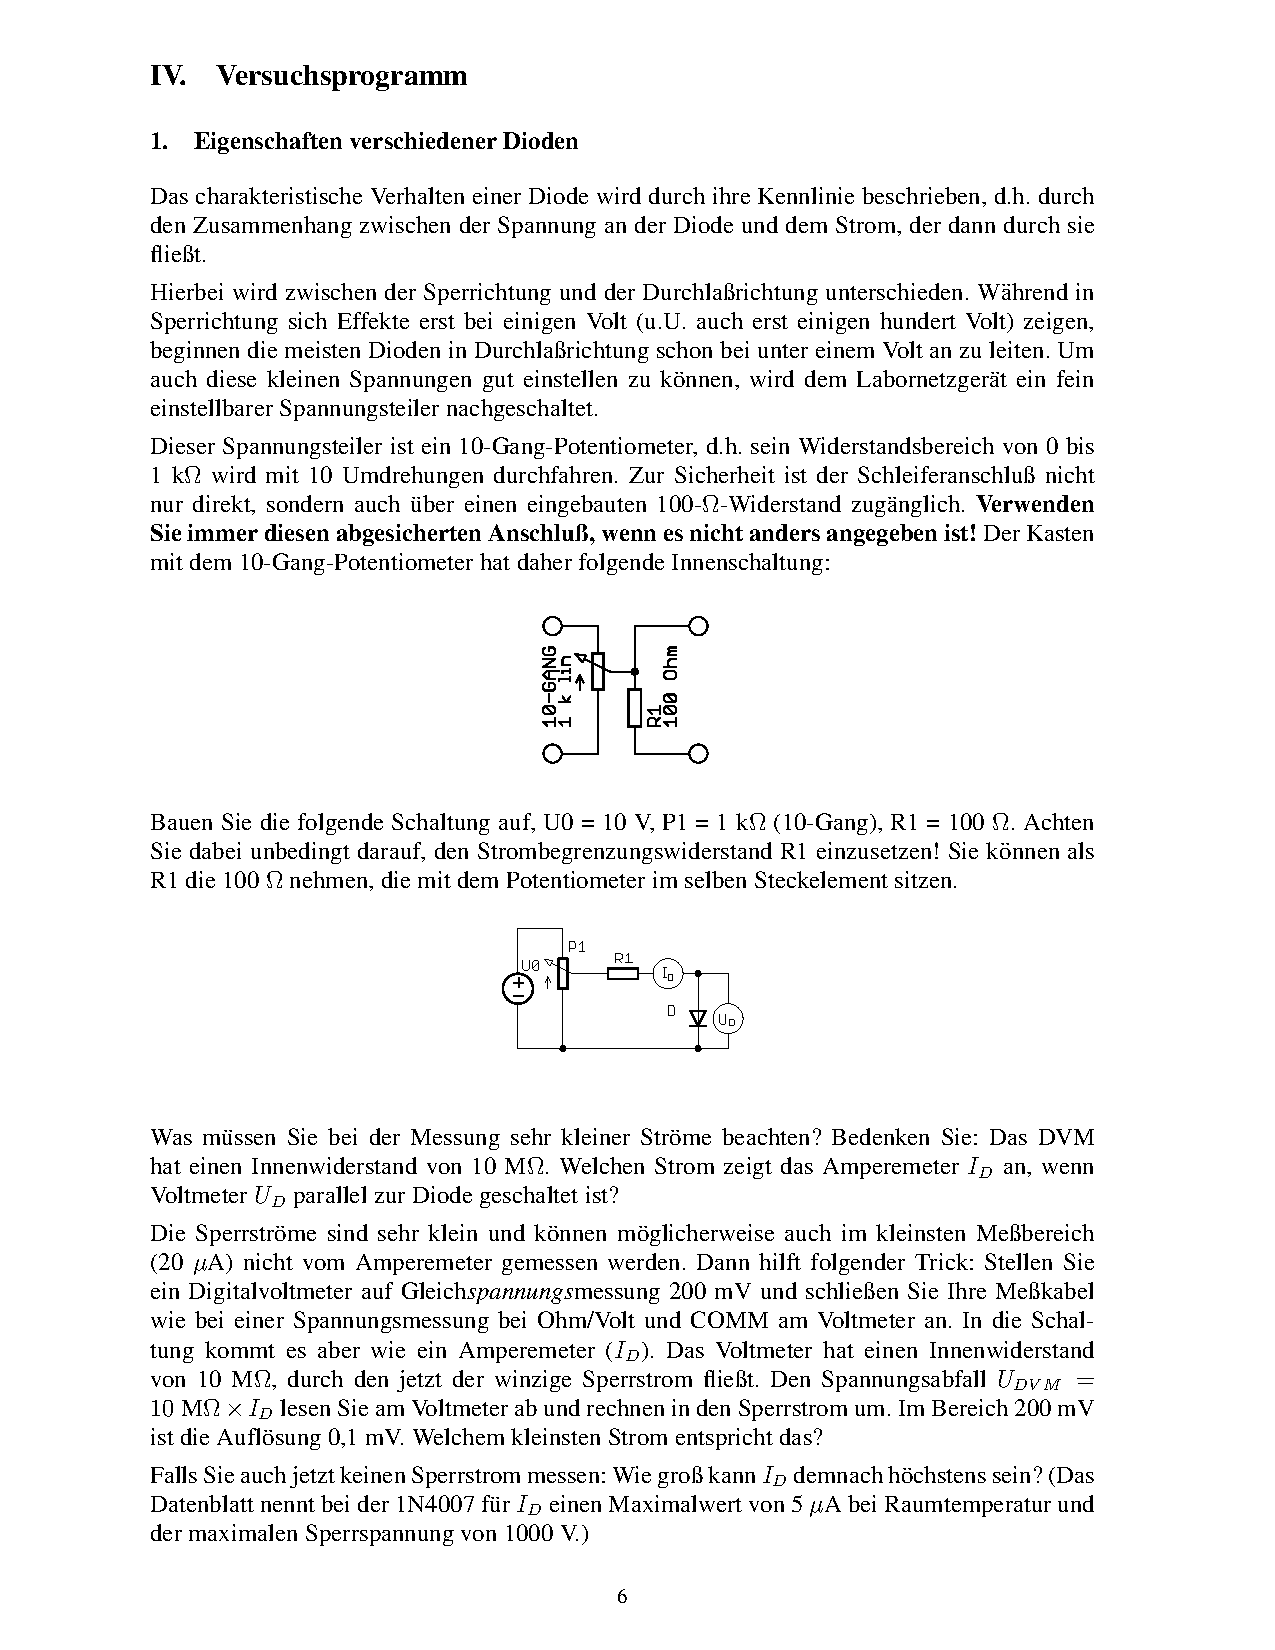
\includegraphics[trim = 10mm 100mm 10mm 155mm, clip, scale = 1]{ep2_14[Page6].pdf}
  	\caption[Schaltskizze für die Messung der Kennlinie der Dioden]{Schaltskizze für die Messung der Kennlinie der Dioden\footnotemark}
  \label{fig:1}
\end{figure}
\footnotetext{Abbildung entnommen von http://www.atlas.uni-wuppertal.de/$\sim$kind/ep2\_14.pdf Seite 6 am 28.10.2014}


\subsection{Versuchsdurchführung}
%erklären, !was! wir machen, !warum! wir das machen und mit welchem ziel
%(wichtig) präzize erklären, wie bei dem versuch vorgegangen und was gemacht wurde
In diesem Versuchsteil soll die Kennlinie einer Diode Aufgenommen werden (Diodentyp 1N4007, Zenerdiode ZPY51). Die Dioden werden in Durchlassrichtung sowie in Sperrichtung betrieben und die Spannung wird gegen den Strom aufgetragen. Davor muss die Schaltung gemäß Abb. \ref{fig:1} aus dem Versuchsaufbau geschaltet werden. Die Spannung wird mithilfe eines 10 Gang Potentiometers (0-1 k$\Omega)$ als Spannungsteiler reguliert. Nun wird eine Gleichspannung von 10V angelegt (Funktionsgenerator). Der Widerstand R$_1$ begrenzt den Strom durch die Diode, sodass diese nicht überlastet wird. Bei sehr kleinen Strömen muss der Strom, der über den Innenwiderstand des DMM abfällt, von dem gemessenenen Strom nach Formel \ref{eqn:Diodenstrom} abgezogen werden. Die Zenerdiode ist darauf ausgelegt in Sperrichtung betrieben zu werden, weshalb hier auch der Tunneldurchbruch ausgemessen wird. Ohne den Vorwiderstand würde die Diode ebenfalls überlastet werden. In Durchlassrichtung wird eine exponentielle Zunahme des Stromes erwartet. (Formel \ref{eqn:exp_Stromzunahme})
\subsection{Verwendete Formeln}
%eine legende kann angefertigt werden, die selbstverständlichen buchstaben müssen nicht extra erklärt werden
%mit knappen erklärungen die !verwendeten! formeln, sowie die zugehörige fehlerrechnung einfügen.
Für den Betrieb der Diode in Durchlassrichtung wird ein exponentieller Zusammenhang gemäß der Formel
\begin{align}
I = I_0(\exp(\frac{\text{eU}}{\text{kT}})-1)
\label{eqn:exp_Stromzunahme}
\end{align}
erwartet.
Der genaue Diodenstrom $I_D$ ergibt sich aus der Knotenregel:
\begin{align}
I_D = I_{DMM_1}-\frac{U_\text{DMM 2}}{R_i}
\label{eqn:Diodenstrom}
\end{align}
Der Diodenstrom ist gleich dem Strom durch das erste Multimeter(Strommessung) minus dem Strom durch das zweite Multimeter(Spannungsmessung).
Im Fall sehr kleiner Ströme wird die Strommessung mit der Voltanzeige des ersten DMM durchgeführt.
Der Strom $I_\text{DMM 1}$ ergibt sich dann aus der Formel:
\begin{align}
I_{DMM_1} = \frac{U_\text{DMM 1}}{R_\text{i}}
\end{align}
Also Spannung geteilt durch den Innenwiderstand nach dem Ohmschen Gesetz.
Der Innenwiderstand beträgt bei beiden Multimetern \unit[10]{M$\Omega$}.

\newpage

\subsection{Messergebnisse}
%die messwerte in !übersichtlichen! tabellen angegeben
%zu viele kleine tabellen in große tabellen überführen!
%zu große tabellen mit dem [scale]-befehl scalieren oder (falls zu lang) in zwei kleinere tabellen aufteilen
%(wichtig) vor !jeder! tabelle sagen, was gemessen wurde und wie die fehler gewählt wurden und ausreichend !erklären!, !warum! wir unsere fehler grade so gewählt haben

Der Messfehler für die Spannung und den Strom wurden aus der Ableseungenauigkeit und dem angegebenem Fehler bestimmt. Für die Spannung ergabt sich so ein Fehler von 0,6V und für den Strom ein Fehler von 0,6mV.

\begin{table}[H]
\centering
\caption{Messwerte aus der 1N4007 Diode in Durchlassrichtung}
\begin{tabular}{|r|r|}
\hline
\multicolumn{1}{|l|}{Spannung/V} & \multicolumn{1}{l|}{Strom/mA} \\ \hline
0 & 0 \\ \hline
0,5 & 0,1 \\ \hline
0,63 & 2 \\ \hline
0,65 & 3,7 \\ \hline
0,67 & 5,1 \\ \hline
0,68 & 6,3 \\ \hline
0,68 & 7,4 \\ \hline
0,69 & 8,5 \\ \hline
0,7 & 9,7 \\ \hline
0,705 & 10,9 \\ \hline
0,71 & 12,3 \\ \hline
0,715 & 13,8 \\ \hline
0,72 & 15,5 \\ \hline
0,725 & 17,7 \\ \hline
0,73 & 20,3 \\ \hline
0,737 & 23,6 \\ \hline
0,743 & 28 \\ \hline
0,751 & 34,2 \\ \hline
0,761 & 43,7 \\ \hline
0,773 & 60 \\ \hline
0,775 & 64,3 \\ \hline
0,779 & 70,3 \\ \hline
0,782 & 76,9 \\ \hline
0,786 & 84,4 \\ \hline
0,79 & 93 \\ \hline
\end{tabular}
\label{tab:a1_1}
\end{table}

\newpage

Der Fehler der Spannung beträgt jeweils 0,06V. Der Fehler des Stroms liegt bei 3,4$\cdot 10^{-10}$A.


\begin{table}[H]
\caption{Messwerte aus der 1N4007 Diode in Sperrrichtung}
\begin{center}
\begin{tabular}{|r|r|r|}
\hline
\multicolumn{1}{|l|}{Spannung$_\text{Strom}$/V } & \multicolumn{1}{l|}{Spannung/V} & \multicolumn{1}{l|}{Diodenstrom/A} \\ \hline
0,05 & -0,056 & 1,06E-008 \\ \hline
0,27 & 0,246 & 2,4E-009 \\ \hline
0,5 & 0,54 & -0,4E-007 \\ \hline
0,76 & 0,761 & -9,9E-011 \\ \hline
1 & 1,011 & -1,1E-009 \\ \hline
1,25 & 1,254 & -4,0E-010 \\ \hline
1,5 & 1,512 & -1,2E-009 \\ \hline
1,76 & 1,765 & -5,0E-010 \\ \hline
2,01 & 2,01 & 0 \\ \hline
2,27 & 2,26 & 0,1E-008 \\ \hline
2,51 & 2,52 & -0,1E-008 \\ \hline
2,77 & 2,77 & 0 \\ \hline
3,02 & 3,02 & 0 \\ \hline
3,27 & 3,27 & 0 \\ \hline
3,52 & 3,52 & 0 \\ \hline
3,77 & 3,77 & 0 \\ \hline
4,03 & 4,02 & 0,1E-008 \\ \hline
4,28 & 4,28 & 0 \\ \hline
4,53 & 4,53 & 0 \\ \hline
4,78 & 4,79 & -0,1E-008 \\ \hline
5,03 & 5,04 & -0,1E-008 \\ \hline
\end{tabular}
\end{center}
\label{tab:a1_2}
\end{table}

\newpage

Der Fehler des Stroms liegt bei 0,06mA und der Fehler der Spannung liegt bei 0,06V.

\begin{table}[H]
\caption{Messwerte der Zenerdiode in Durchlassrichtung}
\begin{center}
\begin{tabular}{|r|r|}
\hline
\multicolumn{1}{|l|}{Spannung/V} & \multicolumn{1}{l|}{Strom/mA} \\ \hline
0,01 & 0 \\ \hline
0,515 & 0 \\ \hline
0,754 & 1,3 \\ \hline
0,777 & 3,2 \\ \hline
0,787 & 4,7 \\ \hline
0,793 & 5,9 \\ \hline
0,797 & 7,1 \\ \hline
0,801 & 8,2 \\ \hline
0,804 & 9,4 \\ \hline
0,807 & 10,6 \\ \hline
0,811 & 12 \\ \hline
0,814 & 13,6 \\ \hline
0,817 & 15,3 \\ \hline
0,82 & 17,4 \\ \hline
0,823 & 20 \\ \hline
0,827 & 23,2 \\ \hline
0,831 & 27,6 \\ \hline
0,837 & 33,8 \\ \hline
0,842 & 43,2 \\ \hline
0,85 & 59,3 \\ \hline
0,851 & 63,9 \\ \hline
0,852 & 69,8 \\ \hline
0,854 & 76,2 \\ \hline
0,856 & 83,7 \\ \hline
0,858 & 92,2 \\ \hline
\end{tabular}
\end{center}
\label{tab:a2_1}
\end{table}

Der Fehler der Spannung beträgt 0,06V und der Fehler des Stroms beträgt 0,003mA.

\begin{table}[H]
\caption{Messwerte der Zenerdiode in Sperrrichtung}
\begin{center}
\begin{tabular}{|r|r|r|}
\hline
\multicolumn{1}{|l|}{Spannung$_\text{Strom}$/V} & \multicolumn{1}{l|}{Spannung/V} & \multicolumn{1}{l|}{Diodenstrom/mA} \\ \hline
0,02 & -0,02 & 0,4E-007 \\ \hline
0,25 & 0,25 & 0 \\ \hline
0,5 & 0,5 & 0 \\ \hline
0,75 & 0,76 & -0,1E-007 \\ \hline
0,98 & 1,02 & -0,4E-007 \\ \hline
1,2 & 1,31 & -1,1E-007 \\ \hline
1,39 & 1,62 & -2,3E-007 \\ \hline
1,54 & 1,97 & -4,3E-007 \\ \hline
1,66 & 2,35 & -6,9E-007 \\ \hline
1,76 & 2,76 & -10E-007 \\ \hline
1,84 & 3,19 & -13,5E-007 \\ \hline
1,9 & 3,64 & -17,4E-007 \\ \hline
1,94 & 4,09 & -21,5E-007 \\ \hline
1,98 & 4,55 & -25,7E-007 \\ \hline
2,01 & 5,02 & -30,1E-007 \\ \hline
2,05 & 5,49 & -34,4E-007 \\ \hline
2,08 & 5,97 & -38,9E-007 \\ \hline
2,1 & 6,45 & -43,5E-007 \\ \hline
2,12 & 6,94 & -48,2E-007 \\ \hline
2,14 & 7,42 & -52,8E-007 \\ \hline
2,15 & 7,52 & -53,7E-007 \\ \hline
2,155 & 7,62 & -54,65E-007 \\ \hline
2,16 & 7,71 & -55,5E-007 \\ \hline
2,165 & 7,82 & -5,655E-007 \\ \hline
2,17 & 7,9 & -57,3E-007 \\ \hline
2,5 & 2,4 & -2,4 \\ \hline
3 & 13 & -12,9 \\ \hline
3,3 & 32,8 & -32,8 \\ \hline
3,4 & 43 & -42,9 \\ \hline
3,5 & 56,5 & -56,5 \\ \hline
3,6 & 74 & -73,9 \\ \hline
3,7 & 94 & -93,9 \\ \hline
3,8 & 125 & -124,9 \\ \hline
3,9 & 165 & -164,9 \\ \hline
4 & 215 & -214,9 \\ \hline
4,2 & 364 & -363,9 \\ \hline
4,4 & 6,42 & -6,4 \\ \hline
4,6 & 1192 & -1191,9 \\ \hline
4,8 & 2560 & -2559,9 \\ \hline
4,9 & 4070 & -4069,9 \\ \hline
4,95 & 5360 & -5359,9 \\ \hline
5 & 7670 & -7669,9 \\ \hline
5,05 & 11810 & -11809,9 \\ \hline
5,1 & 19140 & -19139,9 \\ \hline
5,15 & 34300 & -34299,9 \\ \hline
5,19 & 48700 & -48699,9 \\ \hline
\end{tabular}
\end{center}
\label{tab:a2_2}
\end{table}



\subsection{Auswertung}
%zuerst !alle! errechneten werte entweder in ganzen sätzen aufzählen, oder in tabellen (übersichtlicher) dargestellen, sowie auf die verwendeten formeln verweisen (die referenzierung der formel kann in der überschrift stehen)
%kurz erwähnen (vor der tabelle), warum wir das ganze ausrechnen bzw. was wir dort ausrechnen
%danach histogramme und plots erstellen, wobei wenn möglich funktionen durch die plots gelegt werden (zur not können auch splines benutzt werden, was aber angegeben werden muss)
%bei fits immer die funktion und das reduzierte chiquadrat mit angegeben, wobei auf verständlichkeit beim entziffern der zehnerpotenzen geachtet werden muss z.b. f(x)=(wert+-fehler)\cdot10^{irgendeine zahl}\cdot x + (wert+-fehler)\cdot10^{irgendeine zahl}
%bei jedem fit erklären, nach welchem zusammenhang gefittet wurde und warum!
%bei plots darauf achten, dass die achsenbeschriftung (auch die tics) die richtige größe haben und die legende im plot nicht die messwerte verdeckt
%kurz die aufgabenstellung abgehandeln

Im ersten Aufgabenteil sollten die Kennlinien einer 1N4007 Diode und einer Zenerdiode aufgenommen werden. Für die 1N4007 Diode ergaben sich die folgenden Graphen. Es wurden e-Funktionen angefittet, um den exponentiellen Verlauf zu verdeutlichen.

\begin{figure}[H]
        \centering
        \begin{subfigure}[b]{0.48\textwidth}
                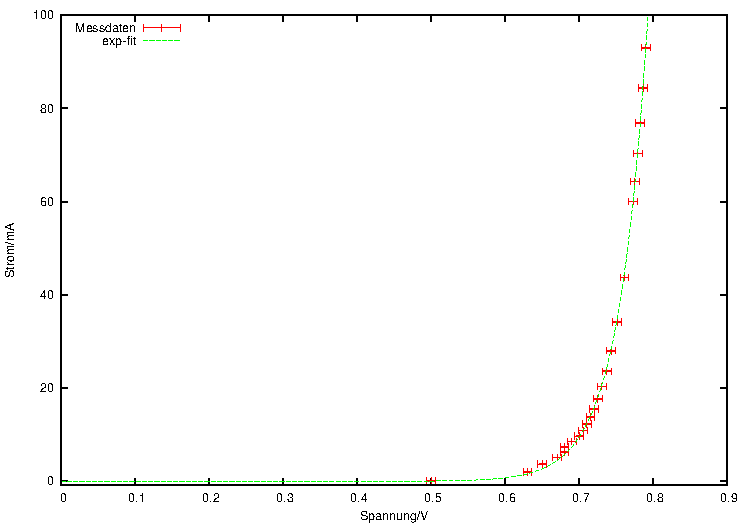
\includegraphics[width=\textwidth , scale = 0.4]{a1_1.pdf}
                \caption[Daten der Messung bei Durchlassrichtung]{Daten der Messung bei Durchlassrichtung}
 				 \label{fig:a1_1}
        \end{subfigure}%
        %~ %add desired spacing between images, e. g. ~, \quad, \qquad, \hfill etc.
          %(or a blank line to force the subfigure onto a new line)
        \hfill
        \begin{subfigure}[b]{0.48\textwidth}
                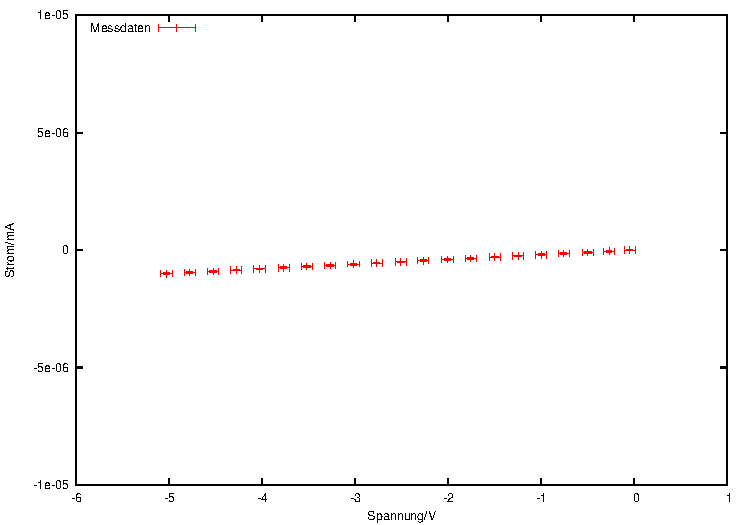
\includegraphics[width=\textwidth , scale = 0.4]{a1_2.pdf}
                \caption[Daten der Messung bei Sperrrichtung]{Daten der Messung bei Sperrrichtung}
  				\label{fig:a1_2}
        \end{subfigure}
        \caption{Kennlinie der 1N4007 Diode}
        \label{fig:a1}
\end{figure}

Für die Zenerdiode ergaben sich die folgenden Graphen aus den Messdaten.

\begin{figure}[H]
        \centering
        \begin{subfigure}[b]{0.48\textwidth}
                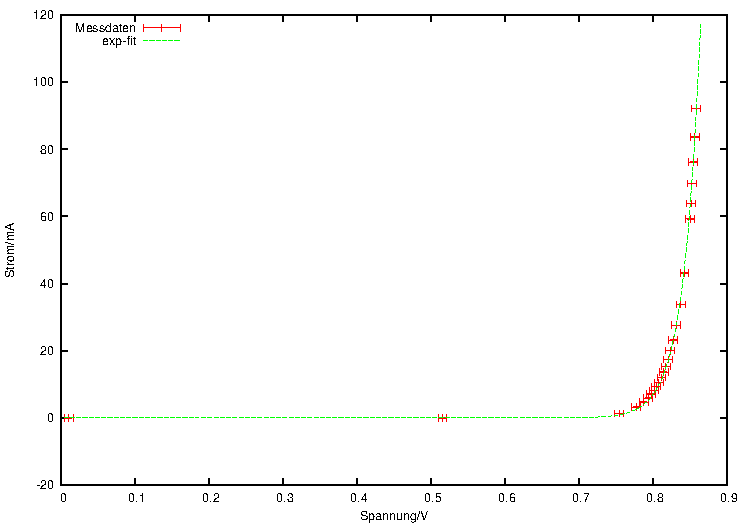
\includegraphics[width=\textwidth , scale = 0.4]{a2_1.pdf}
                \caption[Daten der Messung bei Durchlassrichtung]{Daten der Messung bei Durchlassrichtung}
 				 \label{fig:a2_1}
        \end{subfigure}%
        %~ %add desired spacing between images, e. g. ~, \quad, \qquad, \hfill etc.
          %(or a blank line to force the subfigure onto a new line)
        \hfill
        \begin{subfigure}[b]{0.48\textwidth}
                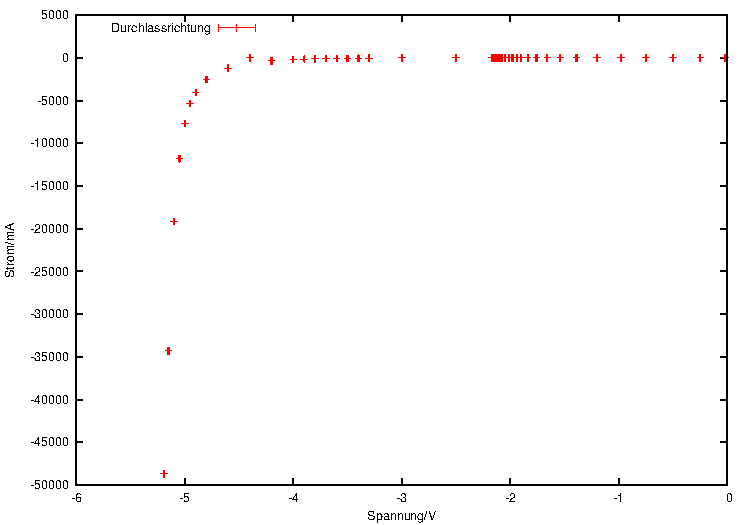
\includegraphics[width=\textwidth , scale = 0.4]{a2_2.pdf}
                \caption[Daten der Messung bei Sperrrichtung]{Daten der Messung bei Sperrrichtung}
  				\label{fig:a2_2}
        \end{subfigure}
        \caption{Kennlinie der Zenerdiode}
        \label{fig:a1}
\end{figure}

Bei der Messung der des Stroms in Sperrrichtung wurde der Diodenstrom aus der Differenz der Ströme durch die beiden DMMs berechnet.

\subsection{Diskussion}
%(immer) die gemessenen werte und die bestimmten werte über die messfehler mit literaturwerten oder untereinander vergleichen
%in welchem fehlerintervall des messwertes liegt der literaturwert oder der vergleichswert?
%wie ist der relative anteil des fehlers am messwert und damit die qualität unserer messung?
%in einem satz erklären, wie gut unser fehler und damit unsere messung ist
%kurz erläutern, wie systematische fehler unsere messung beeinflusst haben könnten
%(wichtig) zum schluss ansprechen, in wie weit die ergebnisse mit der theoretischen vorhersage übereinstimmen
%--------------------------------------------------------------------------------------------
%falls tabellen mit den messwerten zu lang werden, kann die section mit den messwerten auch hinter der diskussion angefügt bzw. eine section mit dem anhang eingefügt werden.
In Abbildung \ref{fig:a1_1} und Abbildung \ref{fig:a2_1} lässt sich gut der exponentielle Anstieg der Stromstärke beobachten. Wie erwarte ist die 1N4007 Diode nahezu Strom undurchlässig, was in \ref{fig:a1_2} zu sehen ist. Bei der Zenerdiode ist der Tunneldurchbruch in Abbildung \ref{fig:a2_2} gut zu erkennen.

\section{Gleichrichterschaltungen}
%kurz das ziel dieses versuchsteiles ansprechen, damit keine zwei überschriften direkt übereinander stehen!
%bei schwierigeren versuchen kann auch der theoretische hintergrund erläutert werden. (mit formeln, herleitungen und erklärungen)
Im zweiten Versuch sollen Schaltungen zur Gleichrichtung des Stromes untersucht werden und miteinander verglichen werden.
\subsection{Verwendete Materialien}
%(immer) eine skizze oder ein foto einfügen, die geräte/materialien !nummerieren! und z.b. eine legende dazu schreiben oder besser noch das ganze in einem Fließtext gut umschreiben
%falls am anfang des versuches nicht klar ist, was alles verwendet wird, wenn möglich erst am ende ein großes foto von den verwendeten materialien machen!

Zur Untersuchung der Ströme und Spannungen werden DMMs und/oder ein Oszilloskop verwendet. Als Stromquellen werden Funktionsgeneratoren oder Transformatoren verwendet. Als Bauteile werden Dioden, Widerstände, Potentiometer, Elektrolytkondenstoren und Glühlampen verwendet.

\subsection{Einweggleichrichtung (Sinusgenerator)}
In diesem Versuchsteil soll das Gleichrichten einer Sinusspannung mittels einer Diode untersucht werden.
\subsubsection{Versuchsaufbau}
%skizze zum versuchsaufbau (oder foto) einfügen,   es muss erklärt werden wie das ganze funktioniert und welche speziellen einstellungen verwendet wurden (z.b. welche knöpfe an den geräten für die messung verdreht wurden)
In diesem Aufbau wird die 1N4007 Diode verwendet. R$_\text{L}$ hat einen Widerstand von 10k$\Omega$. Es werden Frequenzen von 50Hz bis 10kHz durchfahren. Der genaue Aufbau ist Abbildung \ref{fig:2_1} zu entnahmen.

\begin{figure}[H] 
  \centering
    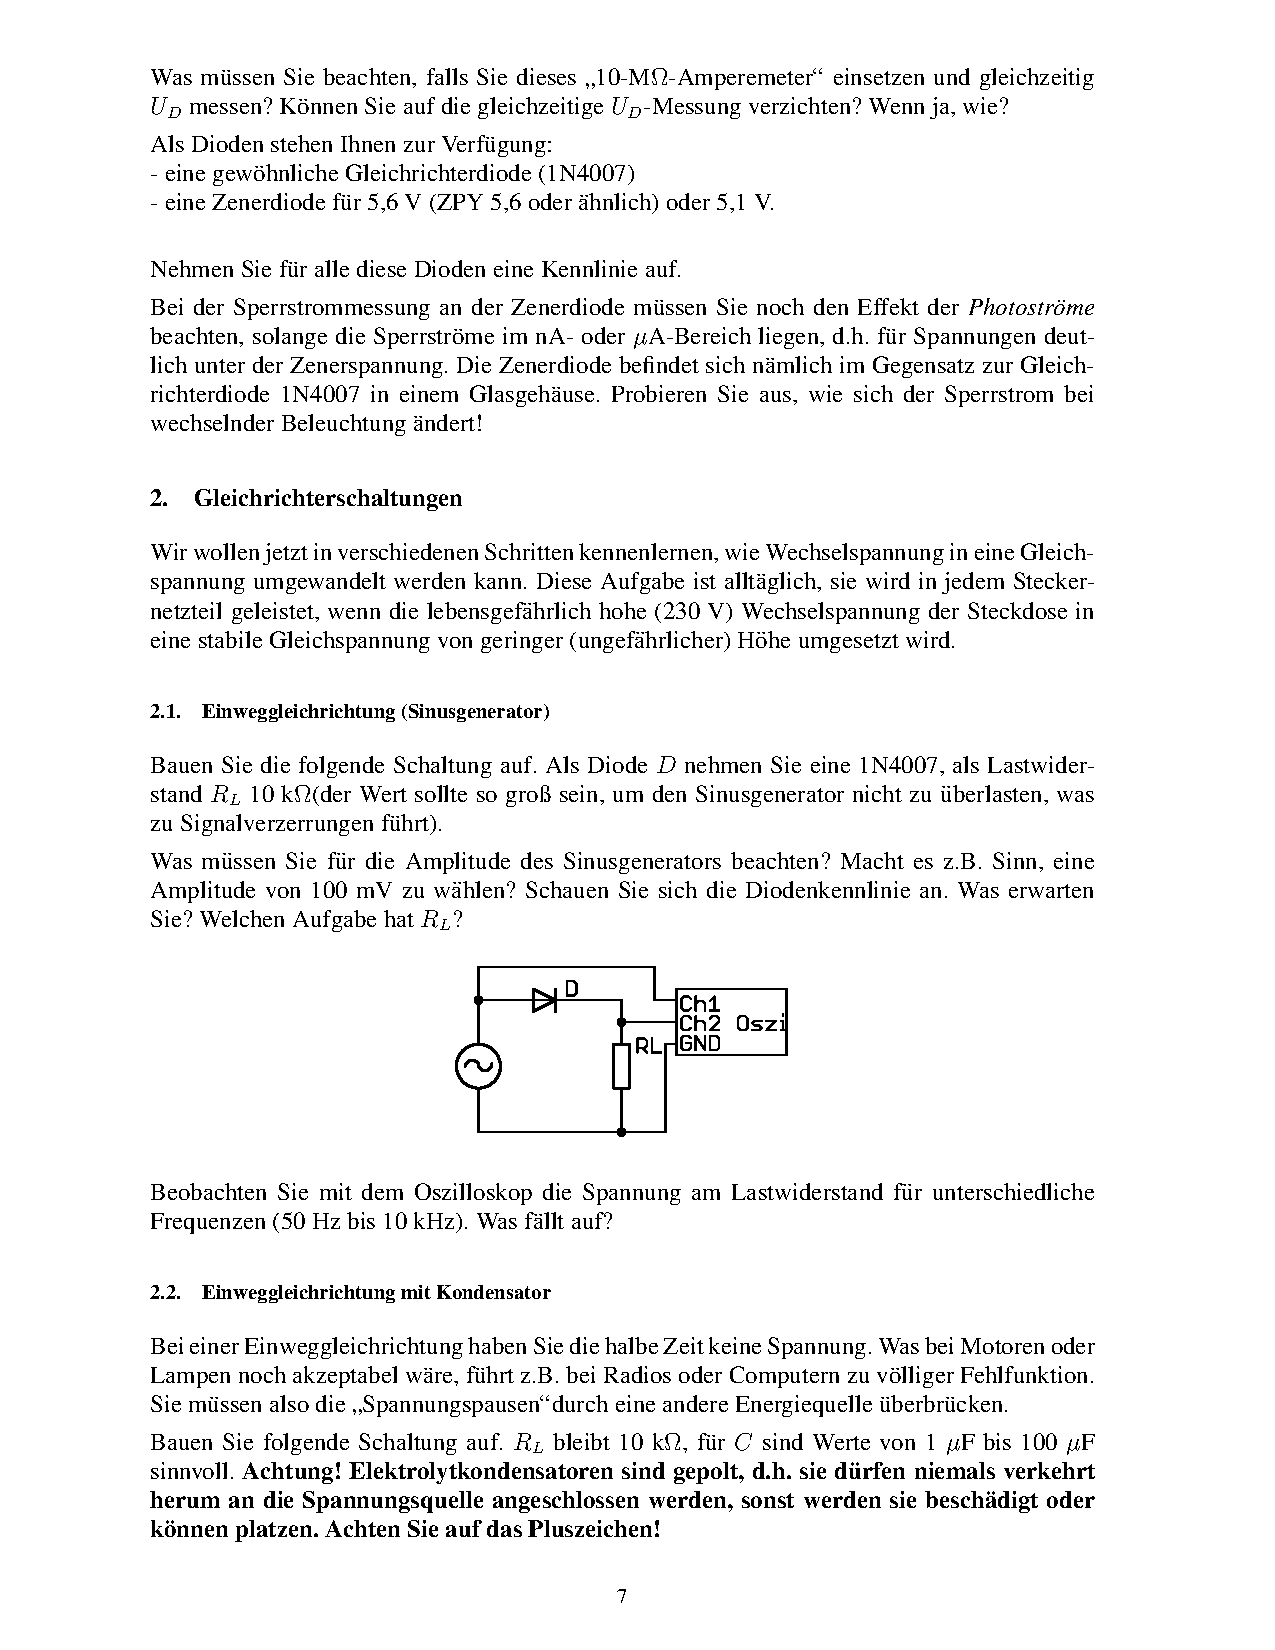
\includegraphics[trim = 10mm 80mm 10mm 160mm, clip, scale = 1]{ep2_14[Page7].pdf}
  	\caption[Schaltskizze für die Messung der Spannung am Lastwiderstand nach vorgeschalteter Diode]{Schaltskizze für die Messung der Spannung am Lastwiderstand nach vorgeschalteter Diode\footnotemark}
  \label{fig:2_1}
\end{figure}
\footnotetext{Abbildung entnommen von http://www.atlas.uni-wuppertal.de/$\sim$kind/ep2\_14.pdf Seite 7 am 28.10.2014}
\subsubsection{Versuchsdurchführung}
%erklären, !was! wir machen, !warum! wir das machen und mit welchem ziel
%(wichtig) präzize erklären, wie bei dem versuch vorgegangen und was gemacht wurde
In diesem Versuchsteil wird eine einfache Diode zum Gleichrichten der Sinusspannung, welche mit dem Funktionsgenerator erzeugt wird, verwendet. Dazu wird Schaltung \ref{fig:2_1} aus dem Versuchsaufbau aufgebaut. Über das Oszilloskop kann die Ausgangsspannung (am Widerstand) mit der Eingangsspannung verglichen werden, wobei ebenso der Wechel- und Gleichspannungsanteil untersucht wird. Die Messung wird dann bei Frequenzen von \unit[50]{Hz}, \unit[1]{kHz} und \unit[10]{kHz} durchgeführt.
\subsubsection{Auswertung}
%zuerst !alle! errechneten werte entweder in ganzen sätzen aufzählen, oder in tabellen (übersichtlicher) dargestellen, sowie auf die verwendeten formeln verweisen (die referenzierung der formel kann in der überschrift stehen)
%kurz erwähnen (vor der tabelle), warum wir das ganze ausrechnen bzw. was wir dort ausrechnen
%danach histogramme und plots erstellen, wobei wenn möglich funktionen durch die plots gelegt werden (zur not können auch splines benutzt werden, was aber angegeben werden muss)
%bei fits immer die funktion und das reduzierte chiquadrat mit angegeben, wobei auf verständlichkeit beim entziffern der zehnerpotenzen geachtet werden muss z.b. f(x)=(wert+-fehler)\cdot10^{irgendeine zahl}\cdot x + (wert+-fehler)\cdot10^{irgendeine zahl}
%bei jedem fit erklären, nach welchem zusammenhang gefittet wurde und warum!
%bei plots darauf achten, dass die achsenbeschriftung (auch die tics) die richtige größe haben und die legende im plot nicht die messwerte verdeckt
%kurz die aufgabenstellung abgehandeln
Bei 50Hz, Abbildung \ref{fig:2_1_1} ist deutlich zu erkennen, dass keine negative Spannung durchgelassen wird. Bei 1kHz, Abbildung \ref{fig:2_1_2} lässt sich ein kleiner Peak in negativer Richtung und bei 10kHz, Abbildung \ref{fig:2_1_3} ein deutlicher Peak erkennen. Dies kommt daher, dass sich die Grenzschicht nicht schnell genug wieder Aufbauen kann und somit für kurze Zeit noch ein Strom in Sperrrichtung fließen kann.

\begin{figure}[H]
        \centering
        \begin{subfigure}[b]{0.28\textwidth}
                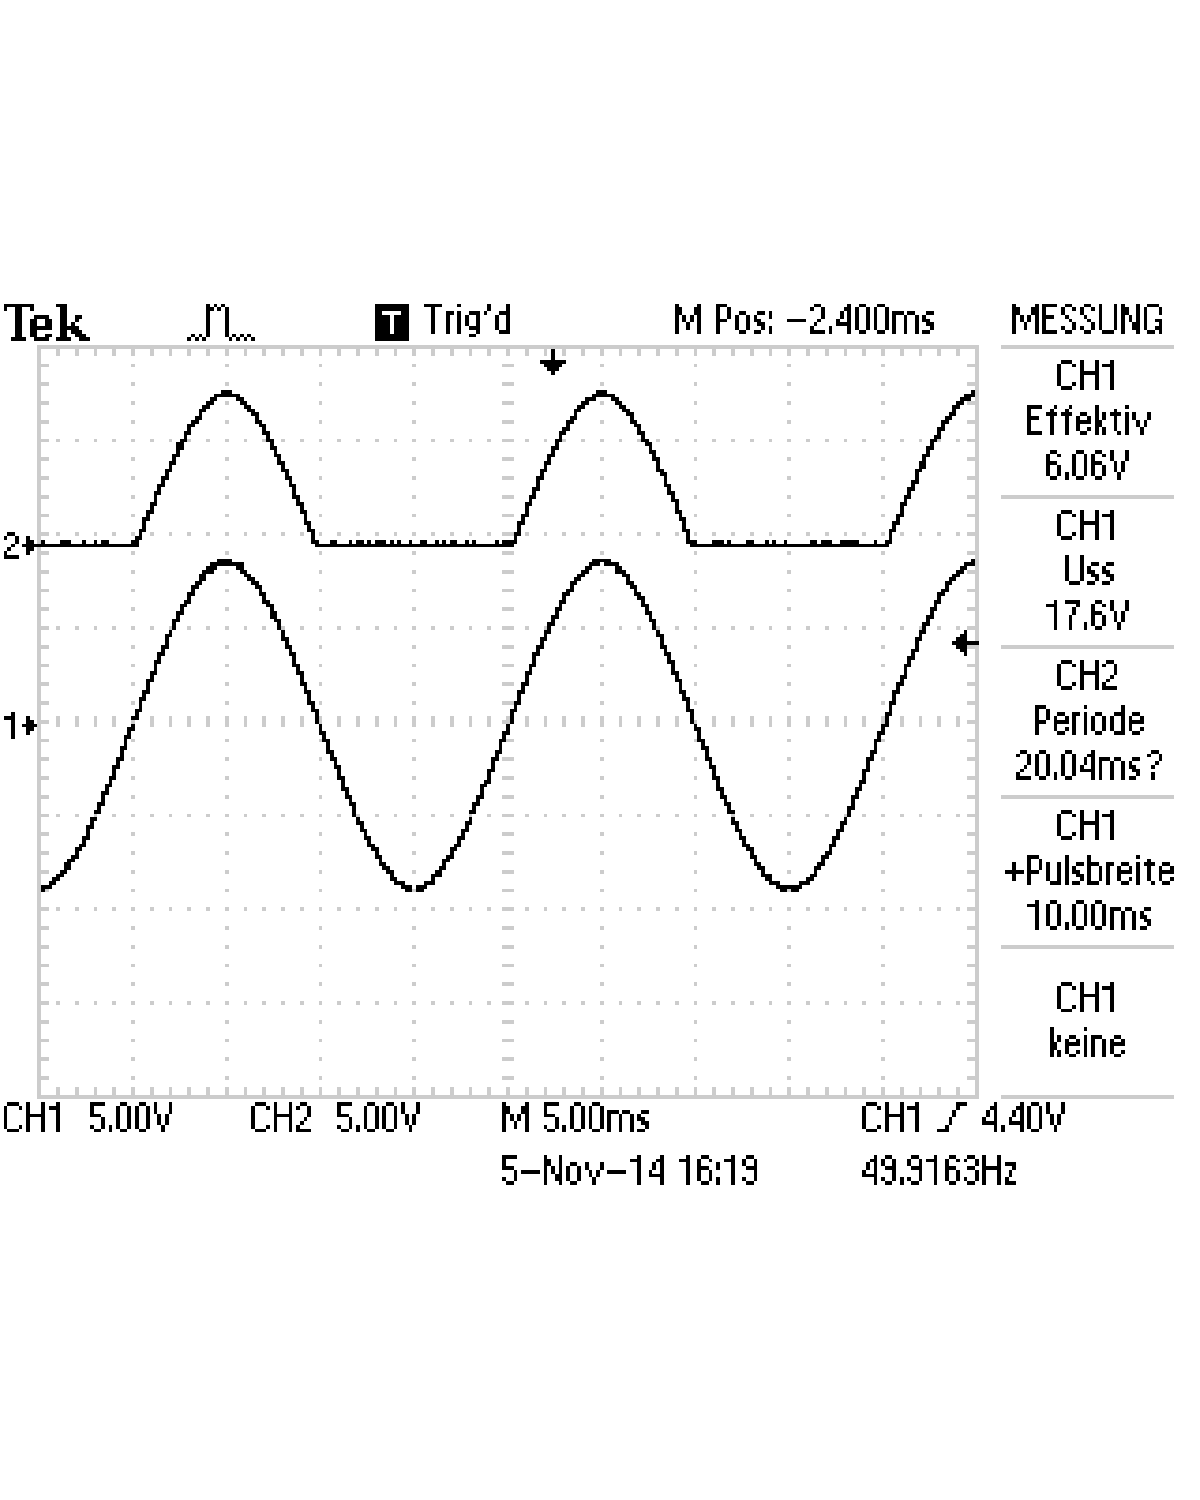
\includegraphics[width=\textwidth , scale = 0.4]{2_1_1.pdf}
                \caption[Aufnahme bei 50Hz]{Aufnahme bei 50Hz}
                \label{fig:2_1_1}
        \end{subfigure}%
       % ~ %add desired spacing between images, e. g. ~, \quad, \qquad, \hfill etc.
          %(or a blank line to force the subfigure onto a new line)
        \hfill
        \begin{subfigure}[b]{0.28\textwidth}
                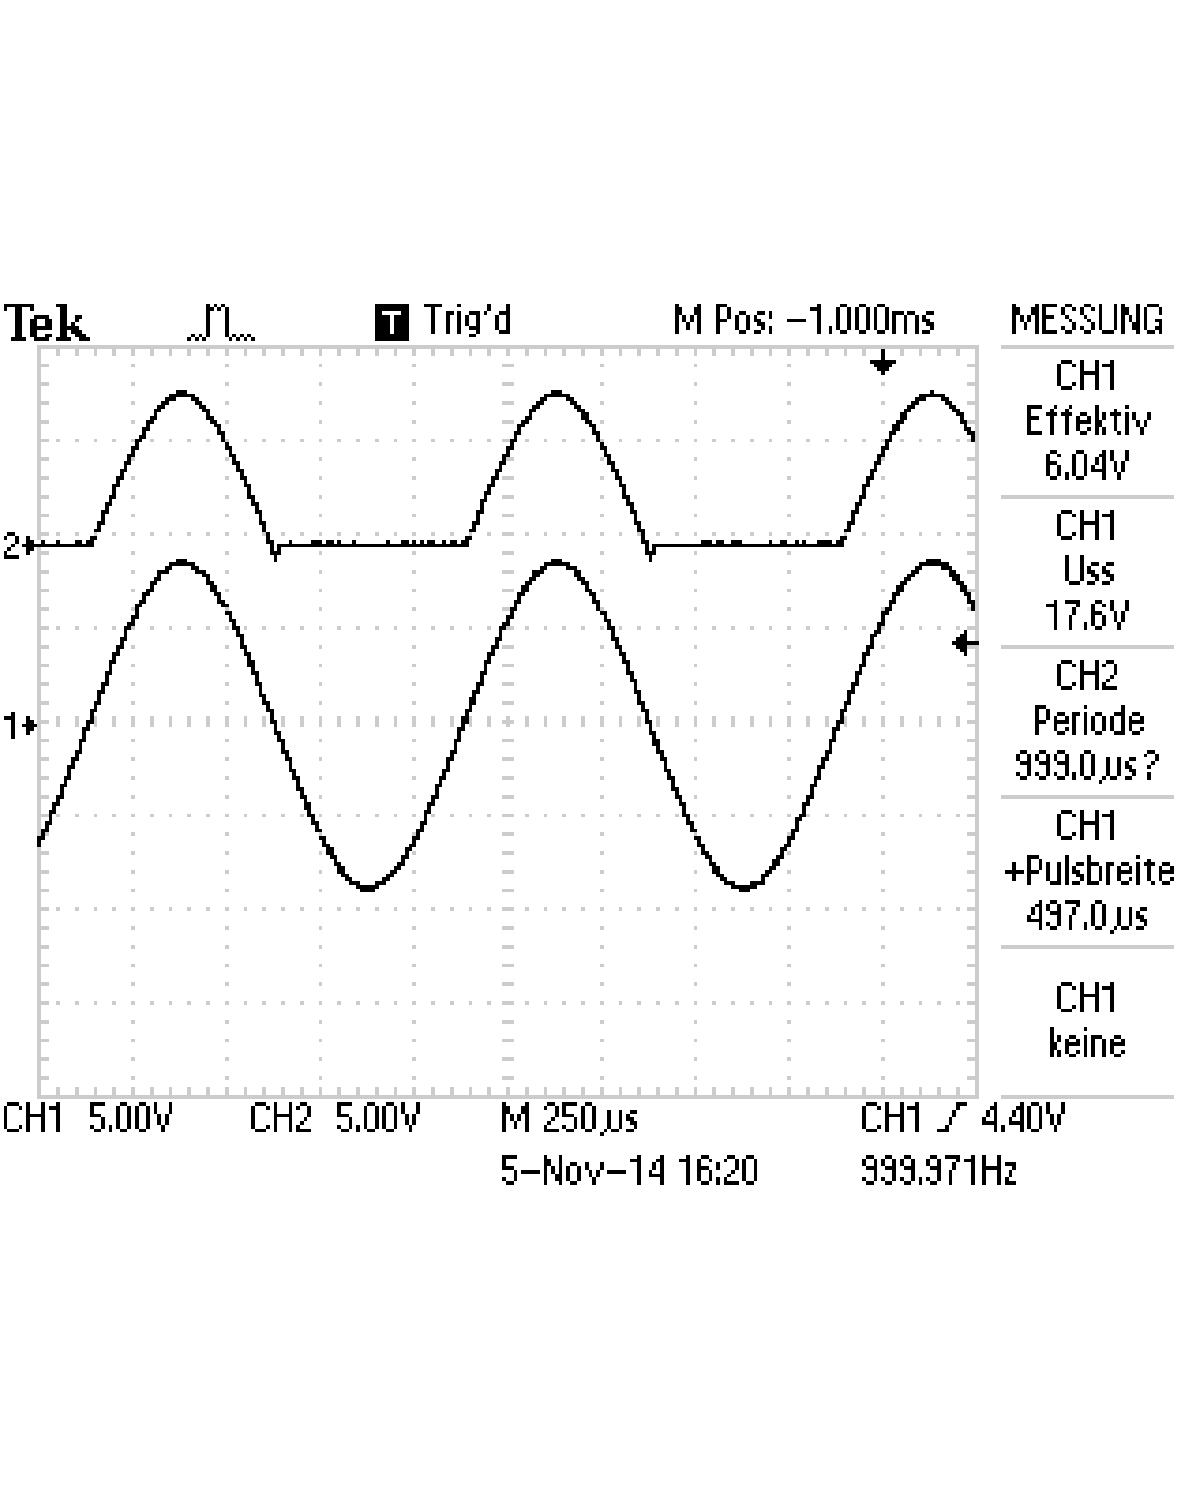
\includegraphics[width=\textwidth , scale = 0.4]{2_1_2.pdf}
                \caption[Aufnahme bei 1kHz]{Aufnahme bei 1kHz}
                \label{fig:2_1_2}
        \end{subfigure}
       % ~ %add desired spacing between images, e. g. ~, \quad, \qquad, \hfill etc.
          %(or a blank line to force the subfigure onto a new line)
        \hfill
        \begin{subfigure}[b]{0.28\textwidth}
        		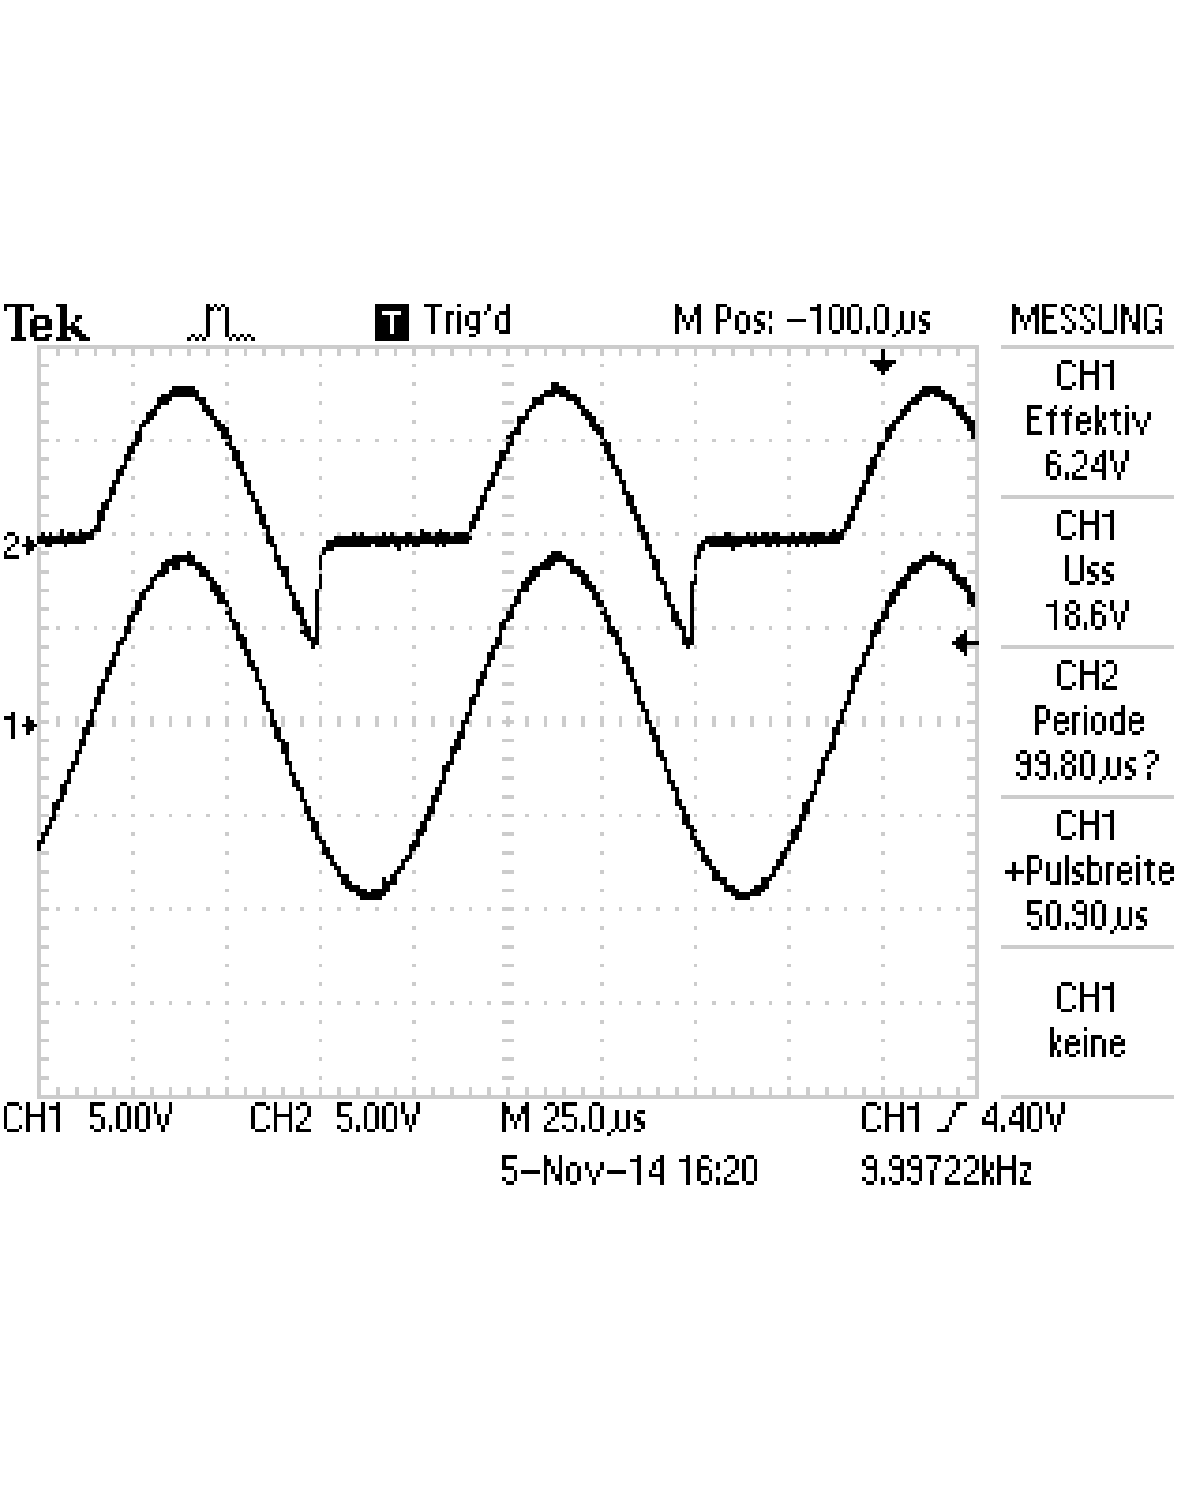
\includegraphics[width=\textwidth, scale = 0.4]{2_1_3.pdf}
                \caption[Aufnahme bei 10kHz]{Aufnahme bei 10kHz}
  				\label{fig:2_1_3}
        \end{subfigure}
        \caption{Aufnahme des Sinussignals bei Einweggleichrichtung für 50Hz, 1kHz und 10kHz}
        \label{fig:2_1_rech_vergleich}
\end{figure}

\subsection{Einweggleichrichtung mit Kondensator}
Zusätzlich zur Diode wird ein Kondensator parallel zur Last geschaltet, um den Spannungsabfall bei negativer Eingangsspannung, bei der die Diode nicht leitet, auszugleichen.
\subsubsection{Versuchsaufbau}
%skizze zum versuchsaufbau (oder foto) einfügen,   es muss erklärt werden wie das ganze funktioniert und welche speziellen einstellungen verwendet wurden (z.b. welche knöpfe an den geräten für die messung verdreht wurden)
Es wird der selbe Versuchsaufbau wie in Abbildung \ref{fig:2_1} Verwendet, jedoch wird ein hinter der Diode liegender Elektrolytkondensator parallel zu R$_\text{L}$ geschaltet. Die Elektrolytkondensator sind dabei im Bereich von 1$\mu$F bis 100$\mu$F zu wählen.
\begin{figure}[H] 
  \centering
    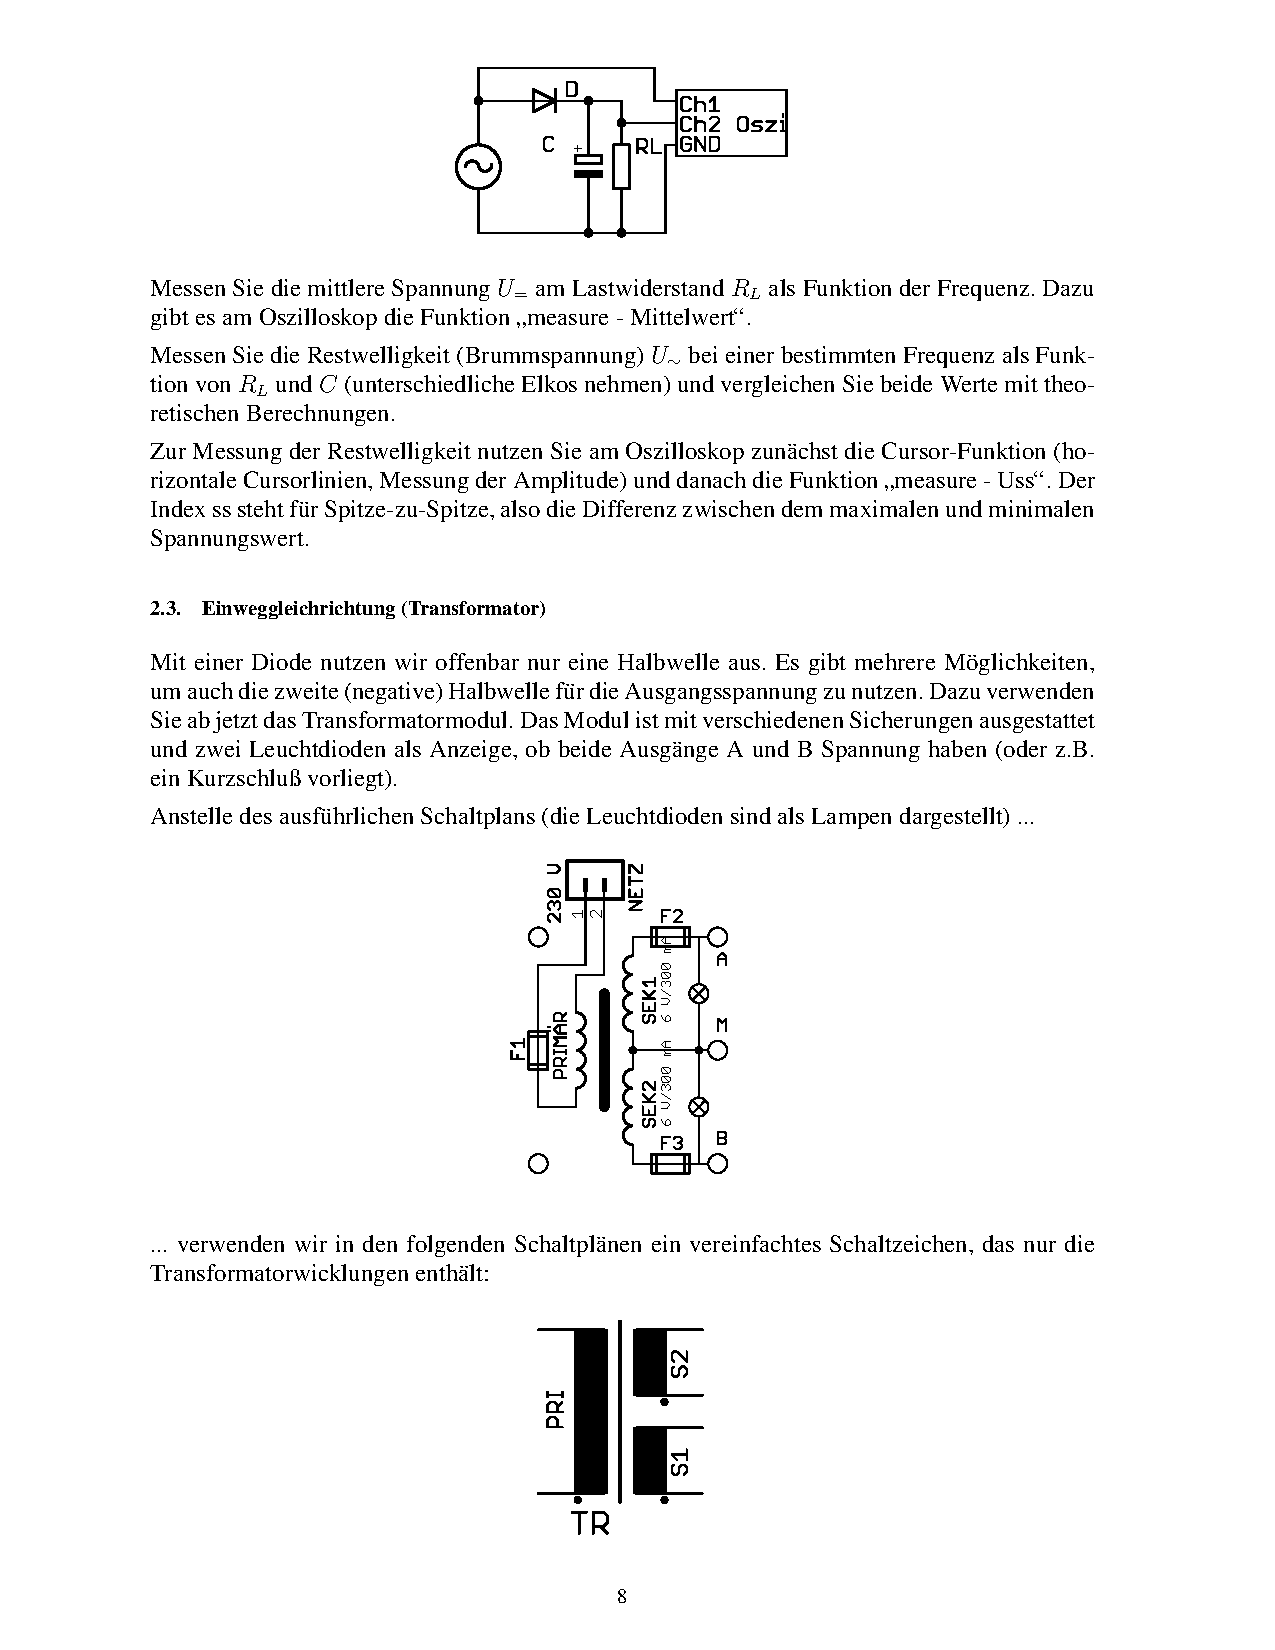
\includegraphics[trim = 10mm 235mm 10mm 10mm, clip, scale = 1]{ep2_14[Page8].pdf}
  	\caption[Schaltskizze für die Messung der Eigenschaften einer Einweggleichrichtungsschaltung mit Kondensator]{Schaltskizze für die Messung der Eigenschaften einer Einweggleichrichtungsschaltung mit Kondensator\footnotemark}
  \label{fig:2_2}
\end{figure}
\footnotetext{Abbildung entnommen von http://www.atlas.uni-wuppertal.de/$\sim$kind/ep2\_14.pdf Seite 8 am 28.10.2014}

\subsubsection{Versuchsdurchführung}
%erklären, !was! wir machen, !warum! wir das machen und mit welchem ziel
%(wichtig) präzize erklären, wie bei dem versuch vorgegangen und was gemacht wurde

In diesem Versuchsteil wird parallel zum Lastwiderstand ein Kondensator geschaltet, der den Spannungsabfall bei negativen Spannungen (durch die Diode fließt kein Strom) verhindern soll \footnote{Versuchsaufbau: Abb. \ref{fig:2_2}}. Für eine Kapazität von \unit[10]{$\mu$F} werden Frequenzen von 20-300\unit{Hz} und für eine Kapazität von \unit[1]{$\mu$F} werden Frequenzen von 20-500\unit{Hz} mit dem Oszilloskop aufgenommen. \footnote{Wechsel- und Gleichspannungsanteil kann abgelesen werden}
\subsubsection{Auswertung}
%zuerst !alle! errechneten werte entweder in ganzen sätzen aufzählen, oder in tabellen (übersichtlicher) dargestellen, sowie auf die verwendeten formeln verweisen (die referenzierung der formel kann in der überschrift stehen)
%kurz erwähnen (vor der tabelle), warum wir das ganze ausrechnen bzw. was wir dort ausrechnen
%danach histogramme und plots erstellen, wobei wenn möglich funktionen durch die plots gelegt werden (zur not können auch splines benutzt werden, was aber angegeben werden muss)
%bei fits immer die funktion und das reduzierte chiquadrat mit angegeben, wobei auf verständlichkeit beim entziffern der zehnerpotenzen geachtet werden muss z.b. f(x)=(wert+-fehler)\cdot10^{irgendeine zahl}\cdot x + (wert+-fehler)\cdot10^{irgendeine zahl}
%bei jedem fit erklären, nach welchem zusammenhang gefittet wurde und warum!
%bei plots darauf achten, dass die achsenbeschriftung (auch die tics) die richtige größe haben und die legende im plot nicht die messwerte verdeckt
%kurz die aufgabenstellung abgehandeln

Der Aufbau wurde mit einem 1$\mu$F und 10$\mu$F aufgebaut und das ankommende Signal bei verschiedenen Frequenzen aufgenommen.

\begin{figure}[H]
        \centering
        \begin{subfigure}[b]{0.48\textwidth}
                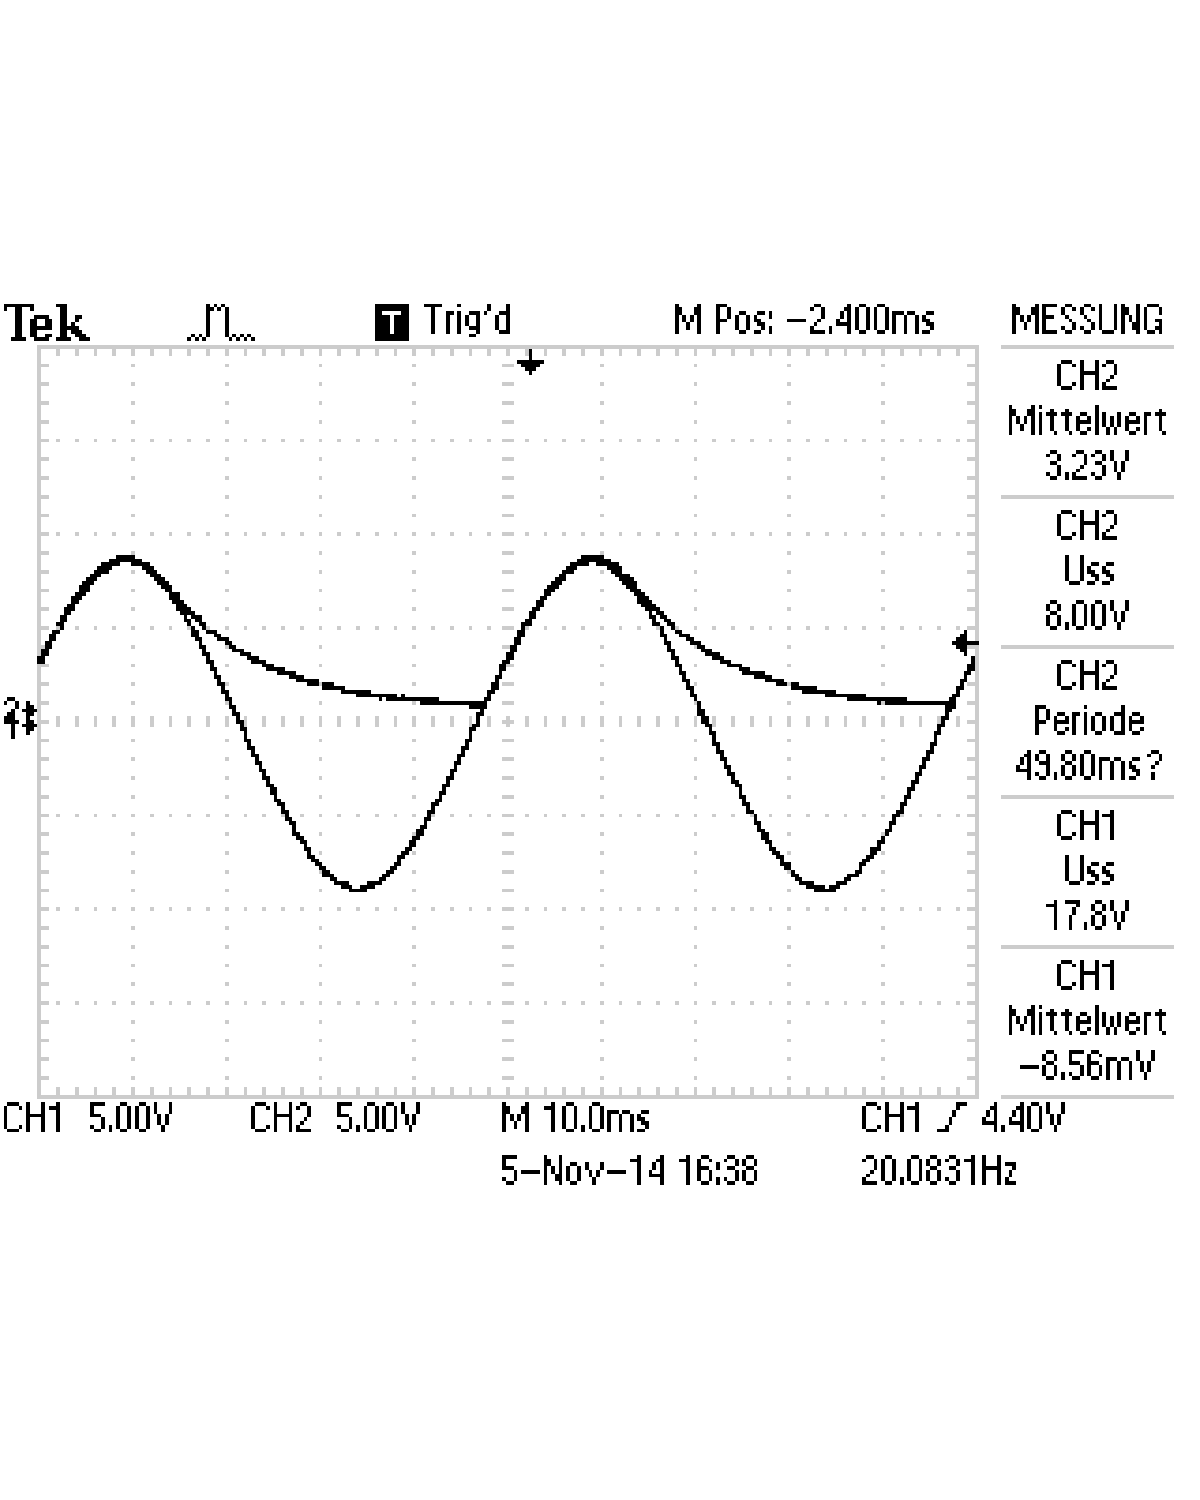
\includegraphics[width=\textwidth , scale = 0.4]{2_2_1F_1.pdf}
                \caption[Aufnahme bei 20Hz]{Aufnahme bei 20Hz}
 				 \label{fig:2_2_1F_1}
        \end{subfigure}%
        %~ %add desired spacing between images, e. g. ~, \quad, \qquad, \hfill etc.
          %(or a blank line to force the subfigure onto a new line)
        \hfill
        \begin{subfigure}[b]{0.48\textwidth}
                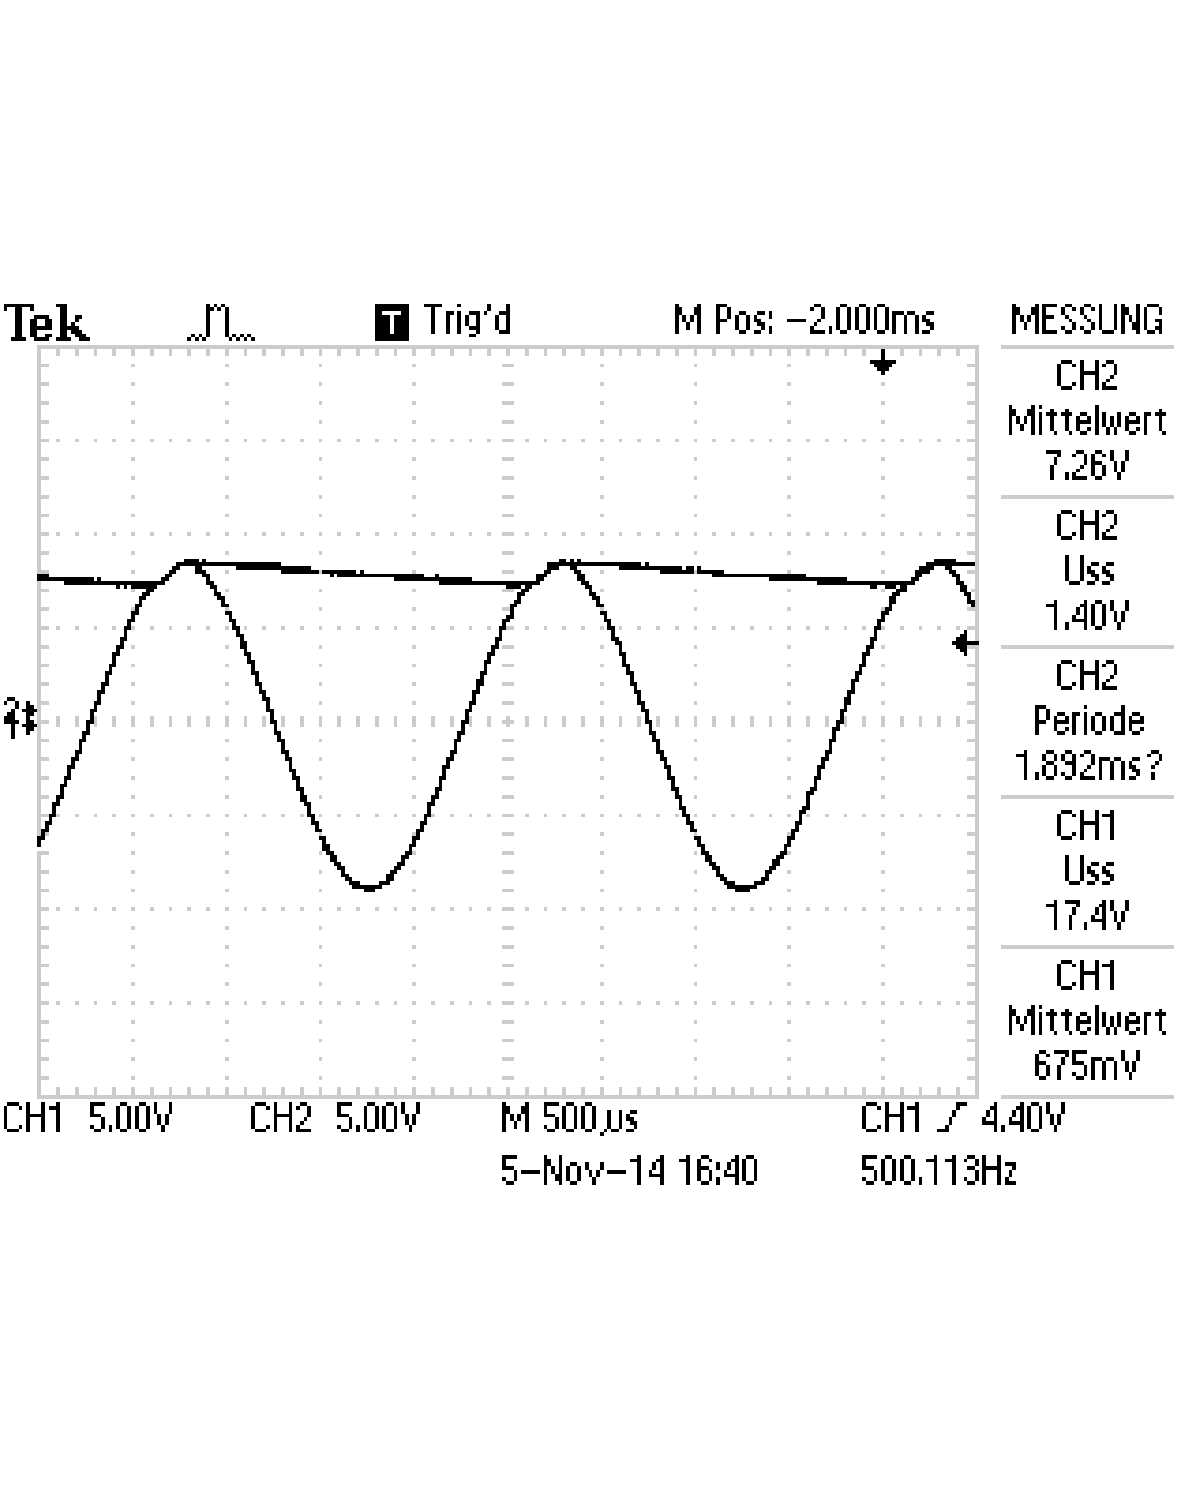
\includegraphics[width=\textwidth , scale = 0.4]{2_2_1F_2.pdf}
                \caption[Aufnahme bei 500Hz]{Aufnahme bei 500Hz}
  				\label{fig:2_2_1F_2}
        \end{subfigure}
        \caption{Aufnahme des ankommenden Signals bei verschiedenen Frequenzen}
        \label{fig:2_2_1F}
\end{figure}

Bei dem 10$\mu$F ergaben sich die folgenden Verläufe auf dem Oszilloskop.

\begin{figure}[H]
        \centering
        \begin{subfigure}[b]{0.48\textwidth}
                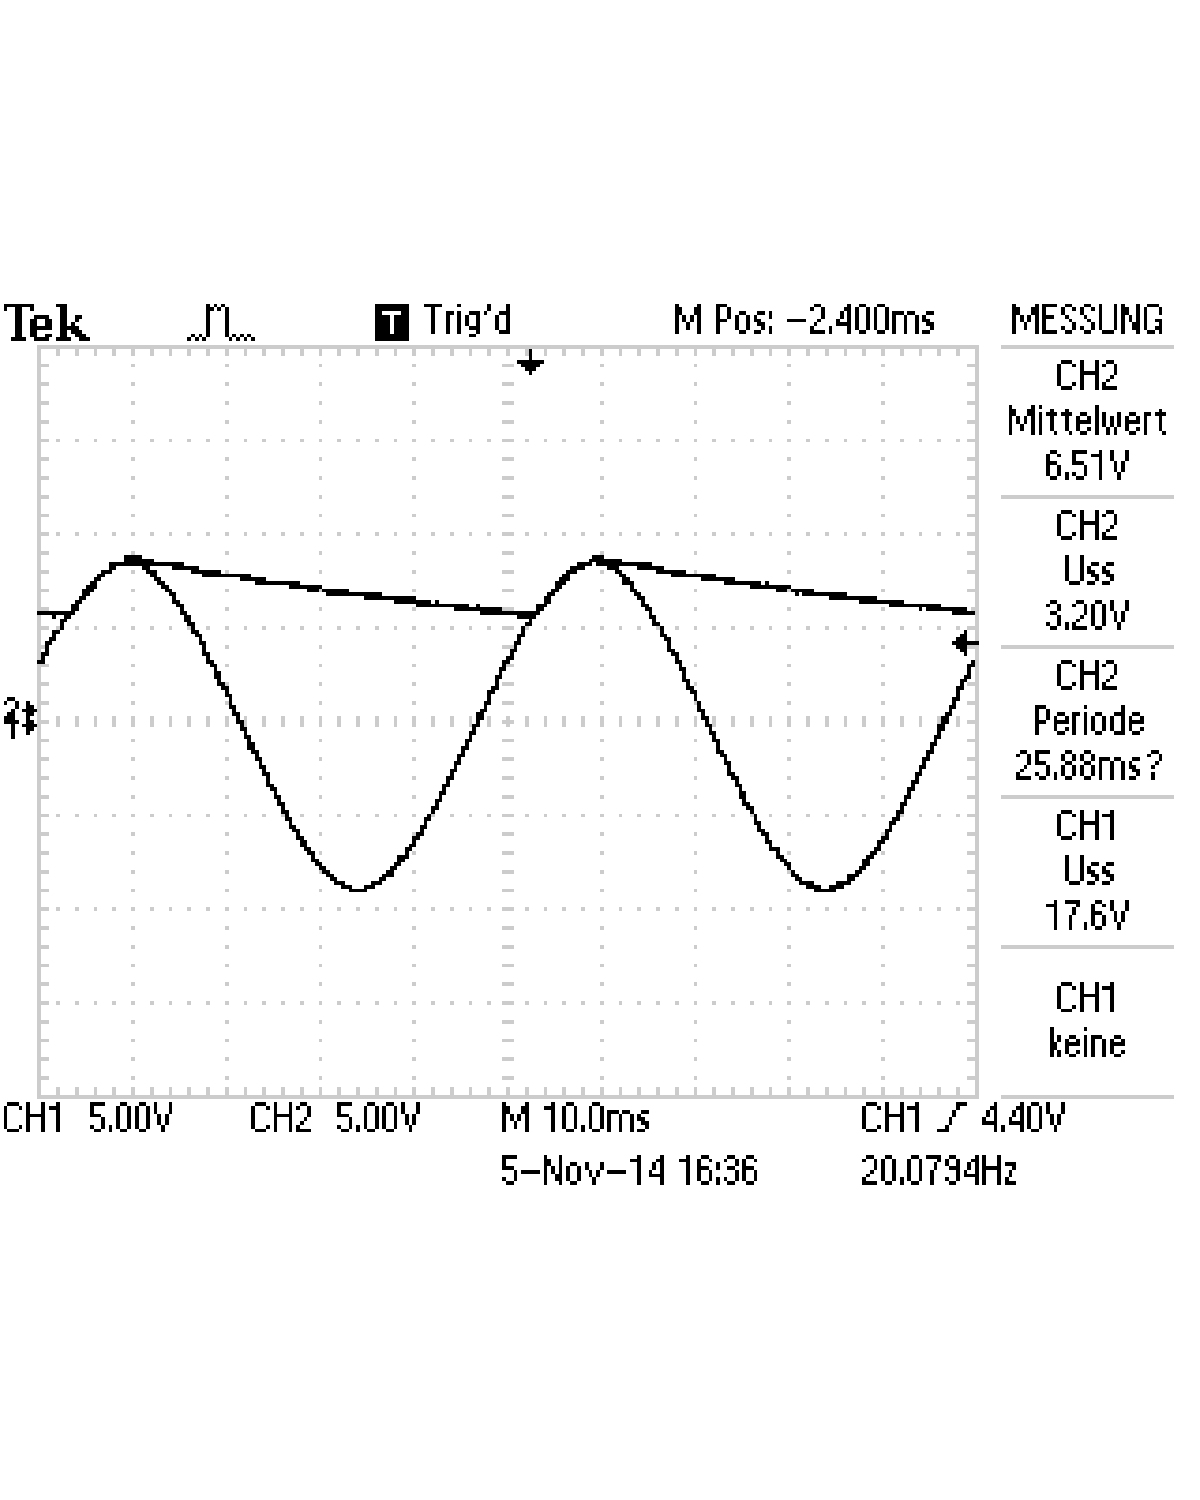
\includegraphics[width=\textwidth , scale = 0.4]{2_2_10F_1.pdf}
                \caption[Aufnahme bei 20Hz]{Aufnahme bei 20Hz}
 				 \label{fig:2_2_10F_1}
        \end{subfigure}%
        %~ %add desired spacing between images, e. g. ~, \quad, \qquad, \hfill etc.
          %(or a blank line to force the subfigure onto a new line)
        \hfill
        \begin{subfigure}[b]{0.48\textwidth}
                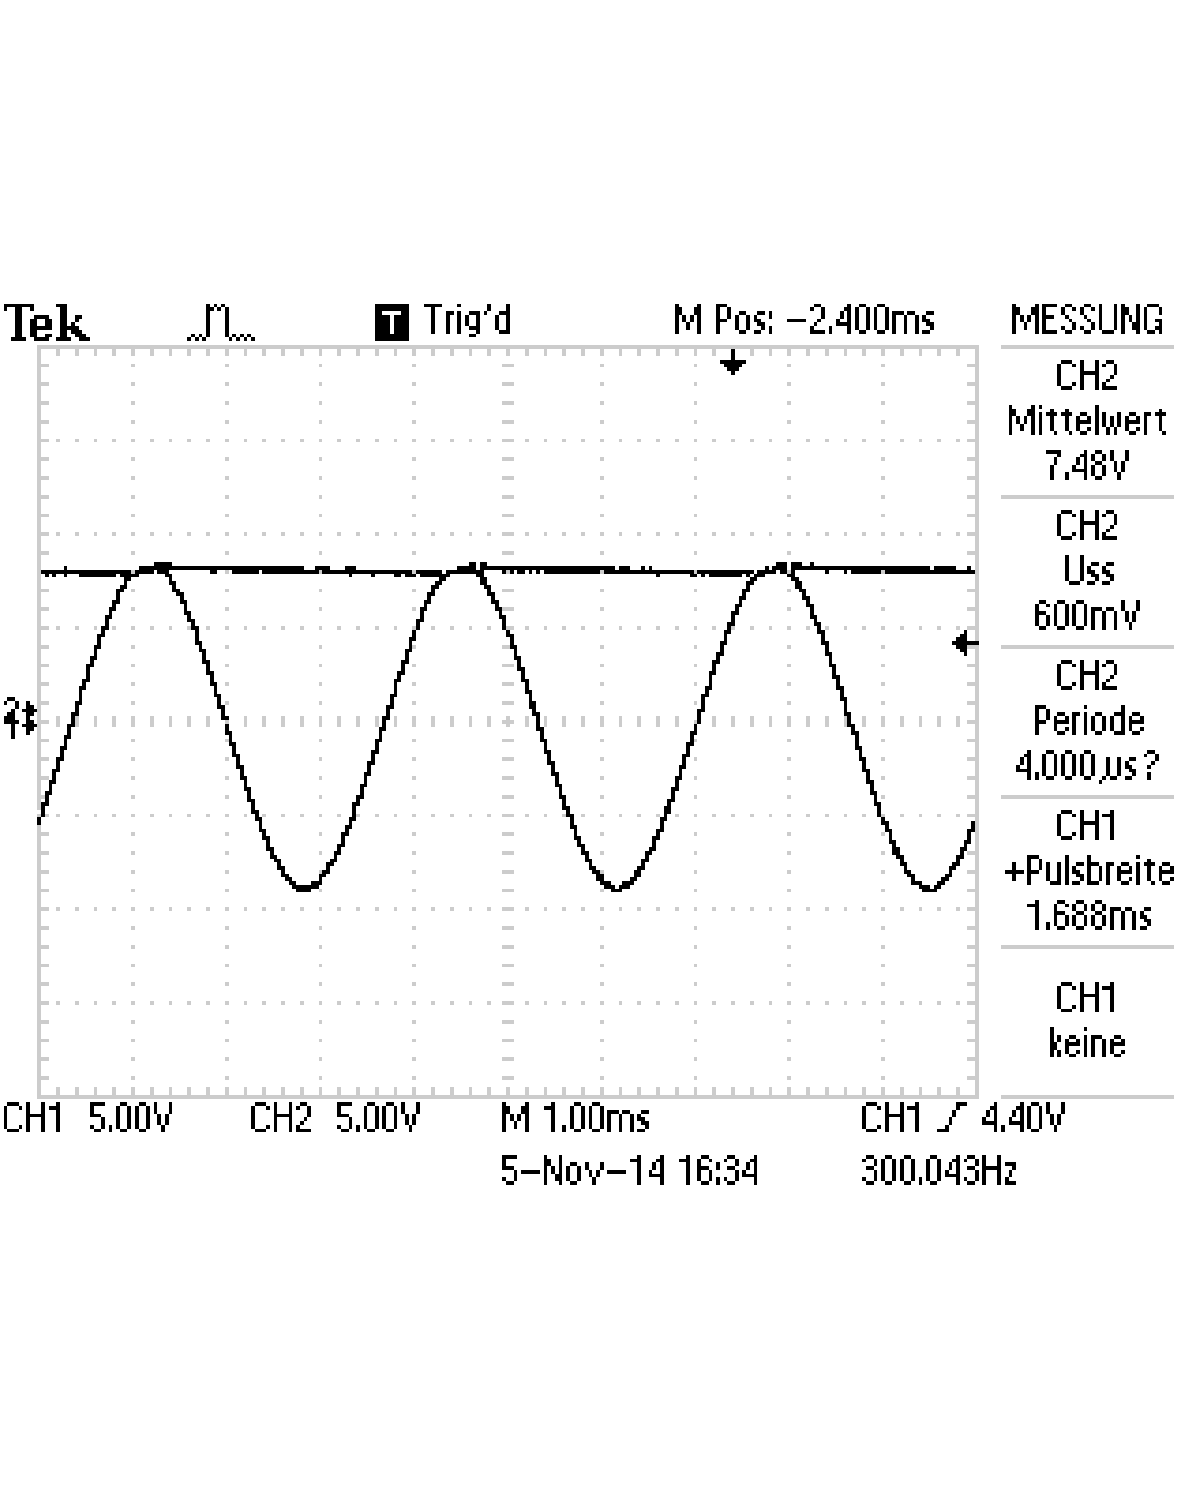
\includegraphics[width=\textwidth , scale = 0.4]{2_2_10F_2.pdf}
                \caption[Aufnahme bei 300Hz]{Aufnahme bei 300Hz}
  				\label{fig:2_2_10F_2}
        \end{subfigure}
        \caption{Aufnahme des ankommenden Signals bei verschiedenen Frequenzen}
        \label{fig:2_2_10F}
\end{figure}

Es ist deutlich zu erkennen, dass bei dem 10$\mu$F Kondensator die Amplitude besser gehalten wird als bei dem 1$\mu$F Kondenstor. Dies liegt and der größeren Halbwertszeit des 10$\mu$F Kondensators.

\subsection{Einweggleichrichtung (Transformator)}
Die durch den Trafo erzeugte Wechselspannung wird wie im vorletzten Versuchsteil ausschließlich mit einer Diode gleichgerichtet.
\subsubsection{Versuchsaufbau}
%skizze zum versuchsaufbau (oder foto) einfügen,   es muss erklärt werden wie das ganze funktioniert und welche speziellen einstellungen verwendet wurden (z.b. welche knöpfe an den geräten für die messung verdreht wurden)


%\begin{figure}[H] 
%  \centering
%    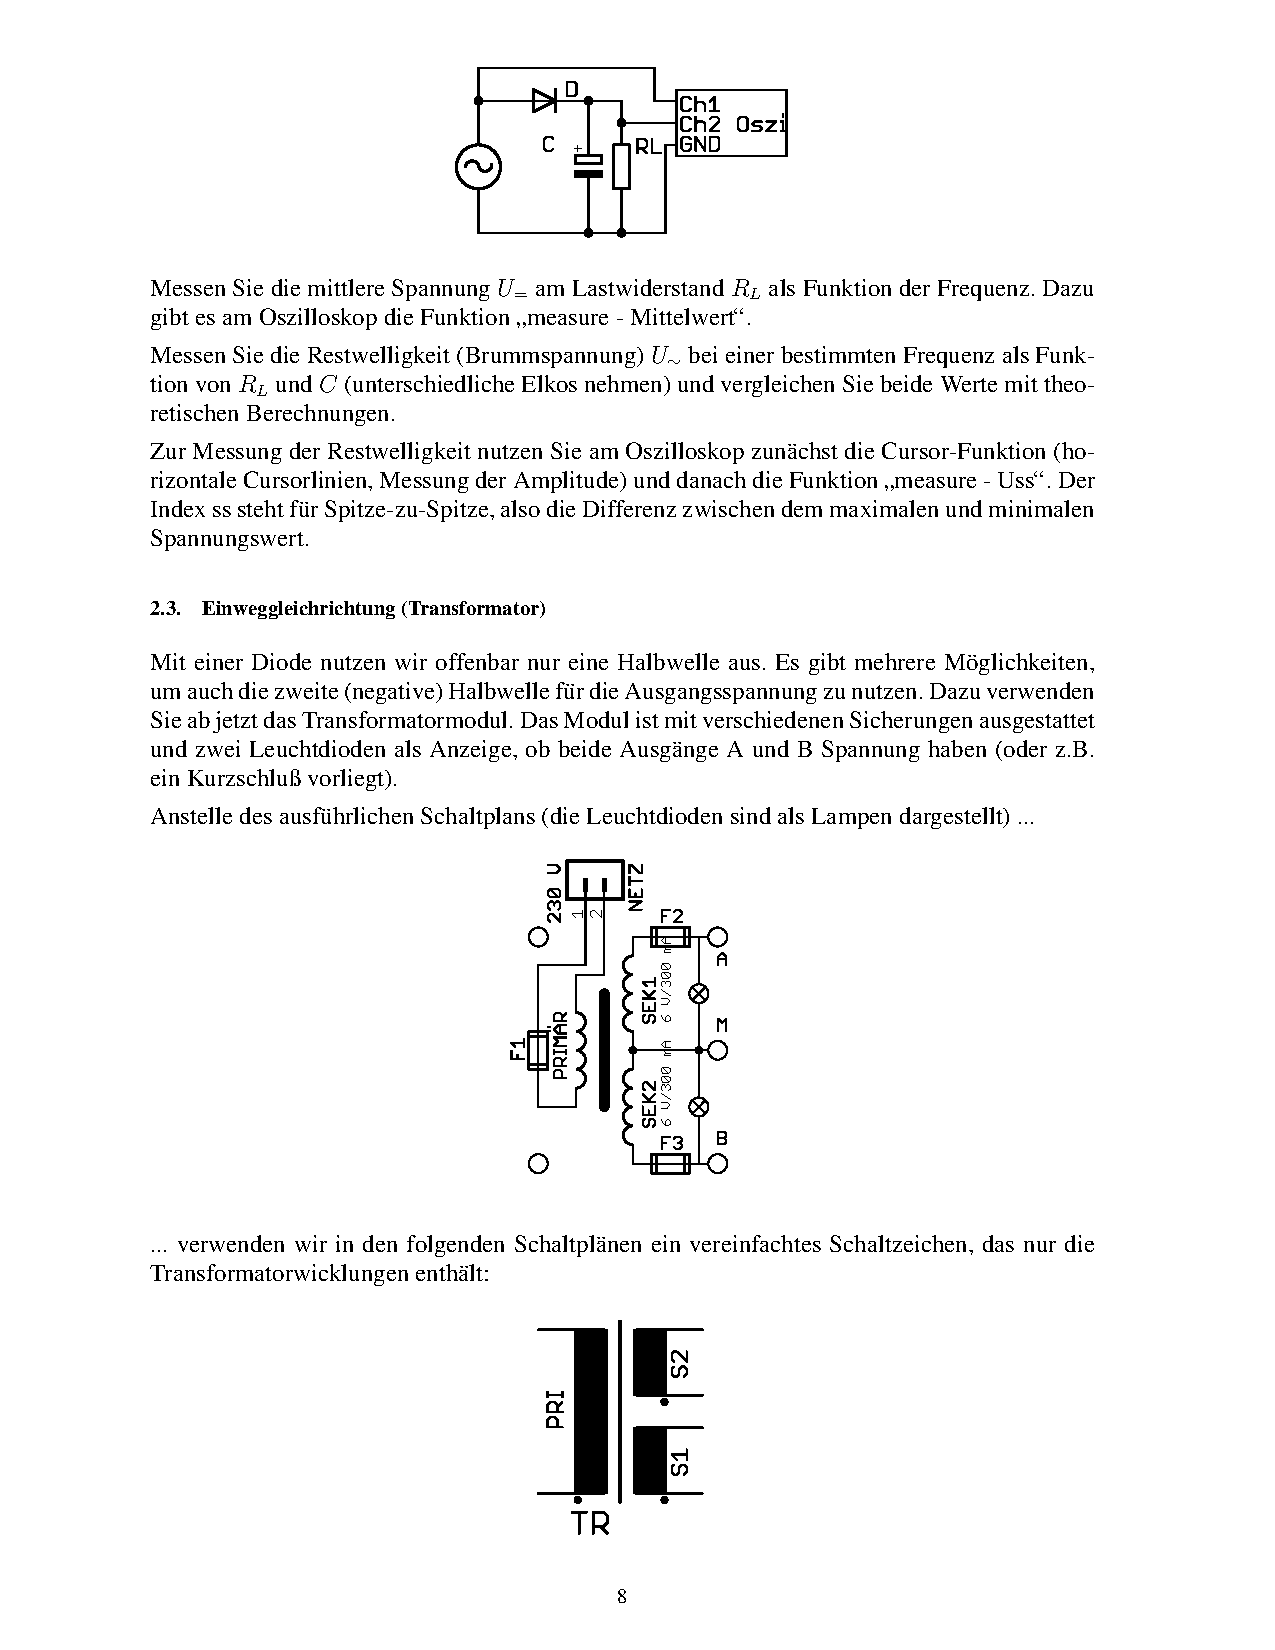
\includegraphics[trim = 10mm 75mm 10mm 145mm, clip, scale = 1]{ep2_14[Page8].pdf}
%  	\caption[Schaltskizze für die Messung der Eigenschaften einer Einweggleichrichtungsschaltung mit Transformator]{Schaltskizze für die Messung der %Eigenschaften einer Einweggleichrichtungsschaltung mit Transformator\footnotemark}
%  \label{fig:2_3}
%\end{figure}
%\footnotetext{Abbildung entnommen von http://www.atlas.uni-wuppertal.de/$\sim$kind/ep2\_14.pdf Seite 8 am 28.10.2014}
In dem Aufbau wird für R$_\text{L}$ ein 470$\Omega$ Potentiometer mit einem 47$\Omega$ Vorwiderstand. Als Diode wird die 1N4007 verwendet. La ist eine Glühlampe und PRI ist ein Transformator, welcher zu Spannungsversorgung verwendet wird.

\begin{figure}[H] 
  \centering
    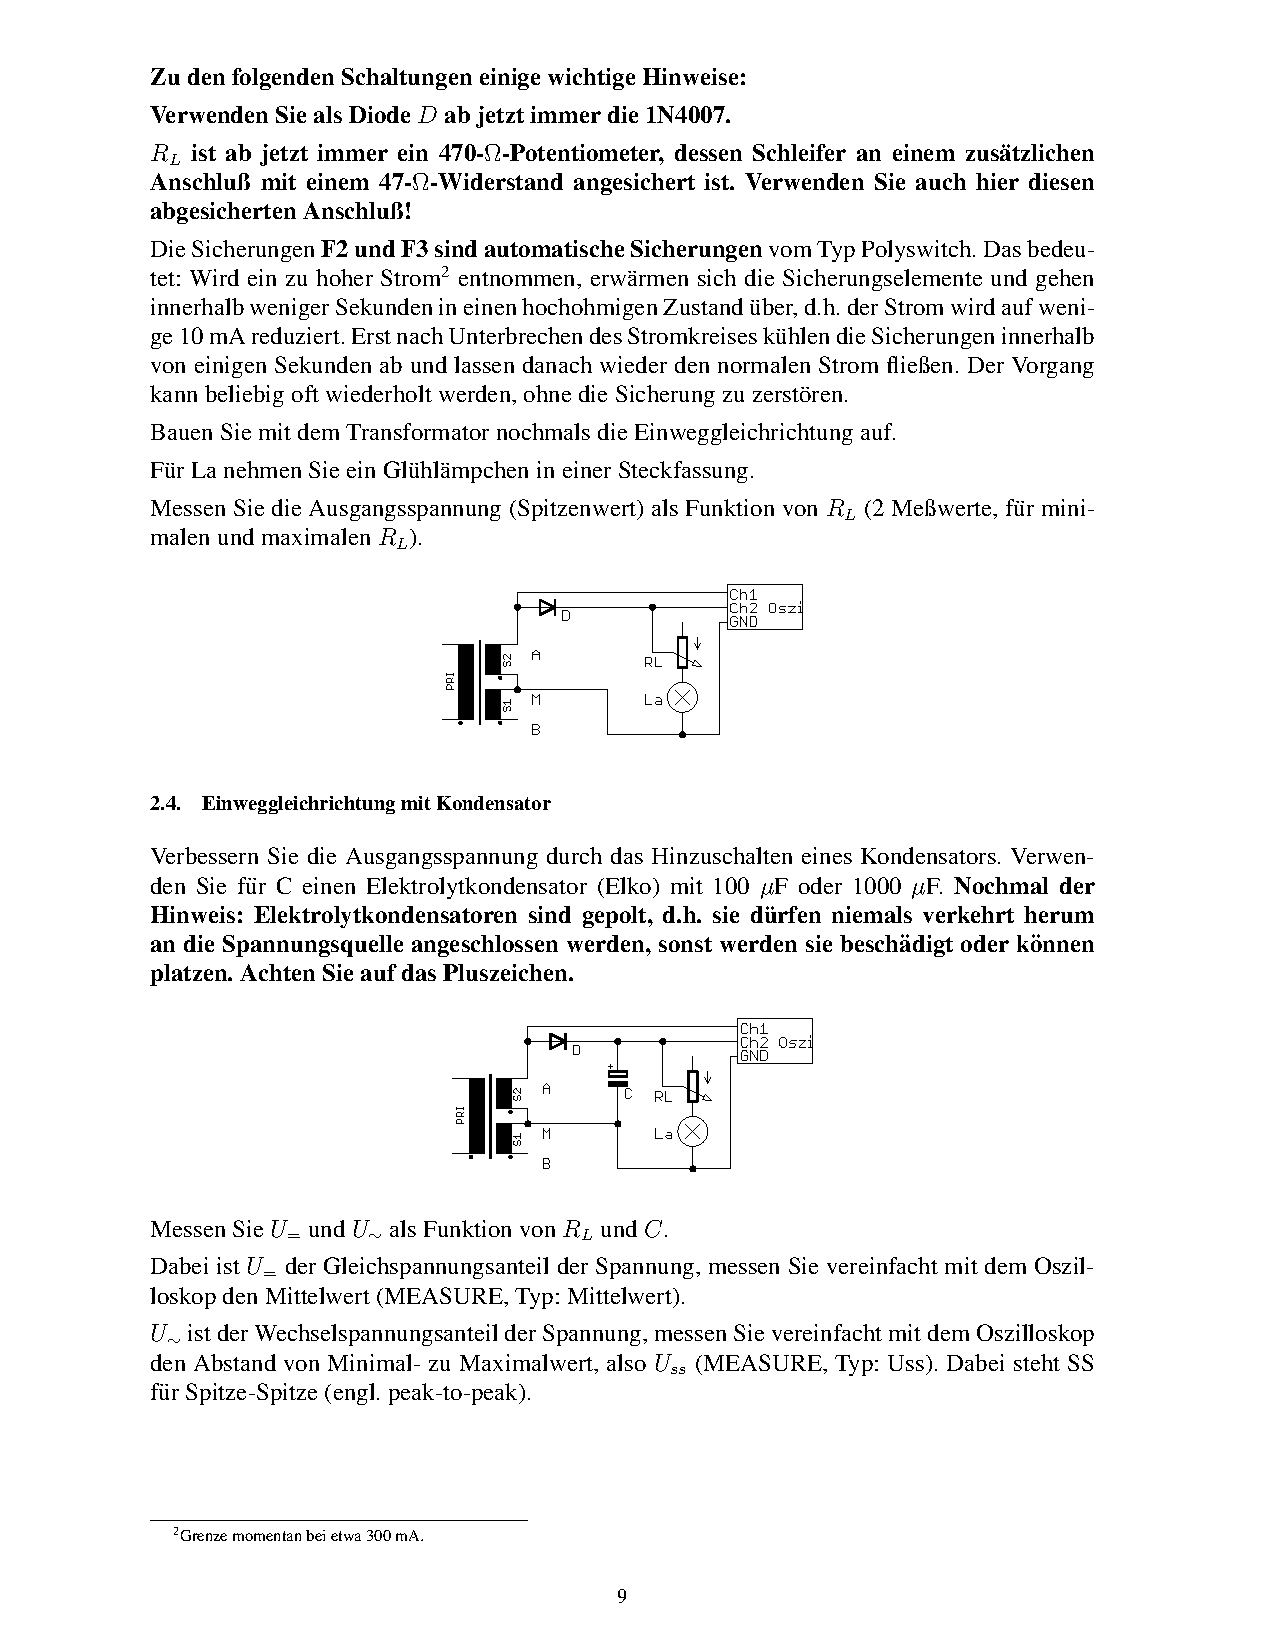
\includegraphics[trim = 10mm 150mm 10mm 95mm, clip, scale = 1]{ep2_14[Page9].pdf}
  	\caption[Schaltskizze zur Einweggleichrichtung mit Transformator]{Schaltskizze zur Einweggleichrichtung mit Transformator\footnotemark}
  \label{fig:2_4}
\end{figure}
\footnotetext{Abbildung entnommen von http://www.atlas.uni-wuppertal.de/$\sim$kind/ep2\_14.pdf Seite 9 am 28.10.2014}

\subsubsection{Versuchsdurchführung}
%erklären, !was! wir machen, !warum! wir das machen und mit welchem ziel
%(wichtig) präzize erklären, wie bei dem versuch vorgegangen und was gemacht wurde
In diesem Versuchsteil wird ein Trafo als Wechselspannungsquelle verwendet \footnote{für Vergleiche mit den nachfolgenden Versuchsteilen wird nur die Hälfte des Trafos als Spannungsquelle benutzt}. Ähnlich wie im ersten Teil wird ausschließlich eine Diode zum Gleichrichten eingesetzt. Als Last wird ein \unit[470]{$\Omega$}Potentiometer mit eingebautem \unit[47]{$\Omega$} Vorwiderstand sowie eine Lampe geschaltet \footnote{Versuchsaufbau: Abb. \ref{fig:2_4}}. Bei maximalem und minimalem Potentiometerwiderstand (47 bzw. \unit[517]{$\Omega$}) wird die Ausgangsspannung auf Wechsel- und Gleichspannungsanteil untersucht.
\subsubsection{Auswertung}
%zuerst !alle! errechneten werte entweder in ganzen sätzen aufzählen, oder in tabellen (übersichtlicher) dargestellen, sowie auf die verwendeten formeln verweisen (die referenzierung der formel kann in der überschrift stehen)
%kurz erwähnen (vor der tabelle), warum wir das ganze ausrechnen bzw. was wir dort ausrechnen
%danach histogramme und plots erstellen, wobei wenn möglich funktionen durch die plots gelegt werden (zur not können auch splines benutzt werden, was aber angegeben werden muss)
%bei fits immer die funktion und das reduzierte chiquadrat mit angegeben, wobei auf verständlichkeit beim entziffern der zehnerpotenzen geachtet werden muss z.b. f(x)=(wert+-fehler)\cdot10^{irgendeine zahl}\cdot x + (wert+-fehler)\cdot10^{irgendeine zahl}
%bei jedem fit erklären, nach welchem zusammenhang gefittet wurde und warum!
%bei plots darauf achten, dass die achsenbeschriftung (auch die tics) die richtige größe haben und die legende im plot nicht die messwerte verdeckt
%kurz die aufgabenstellung abgehandeln

In diesem Aufgabenteil soll die Ausgangsspannung in Abhängigkeit von RL gemessen werden, dafür wurde einmal für RL$_\text{min}$ und für RL$_\text{max}$.

\begin{figure}[H]
        \centering
        \begin{subfigure}[b]{0.48\textwidth}
                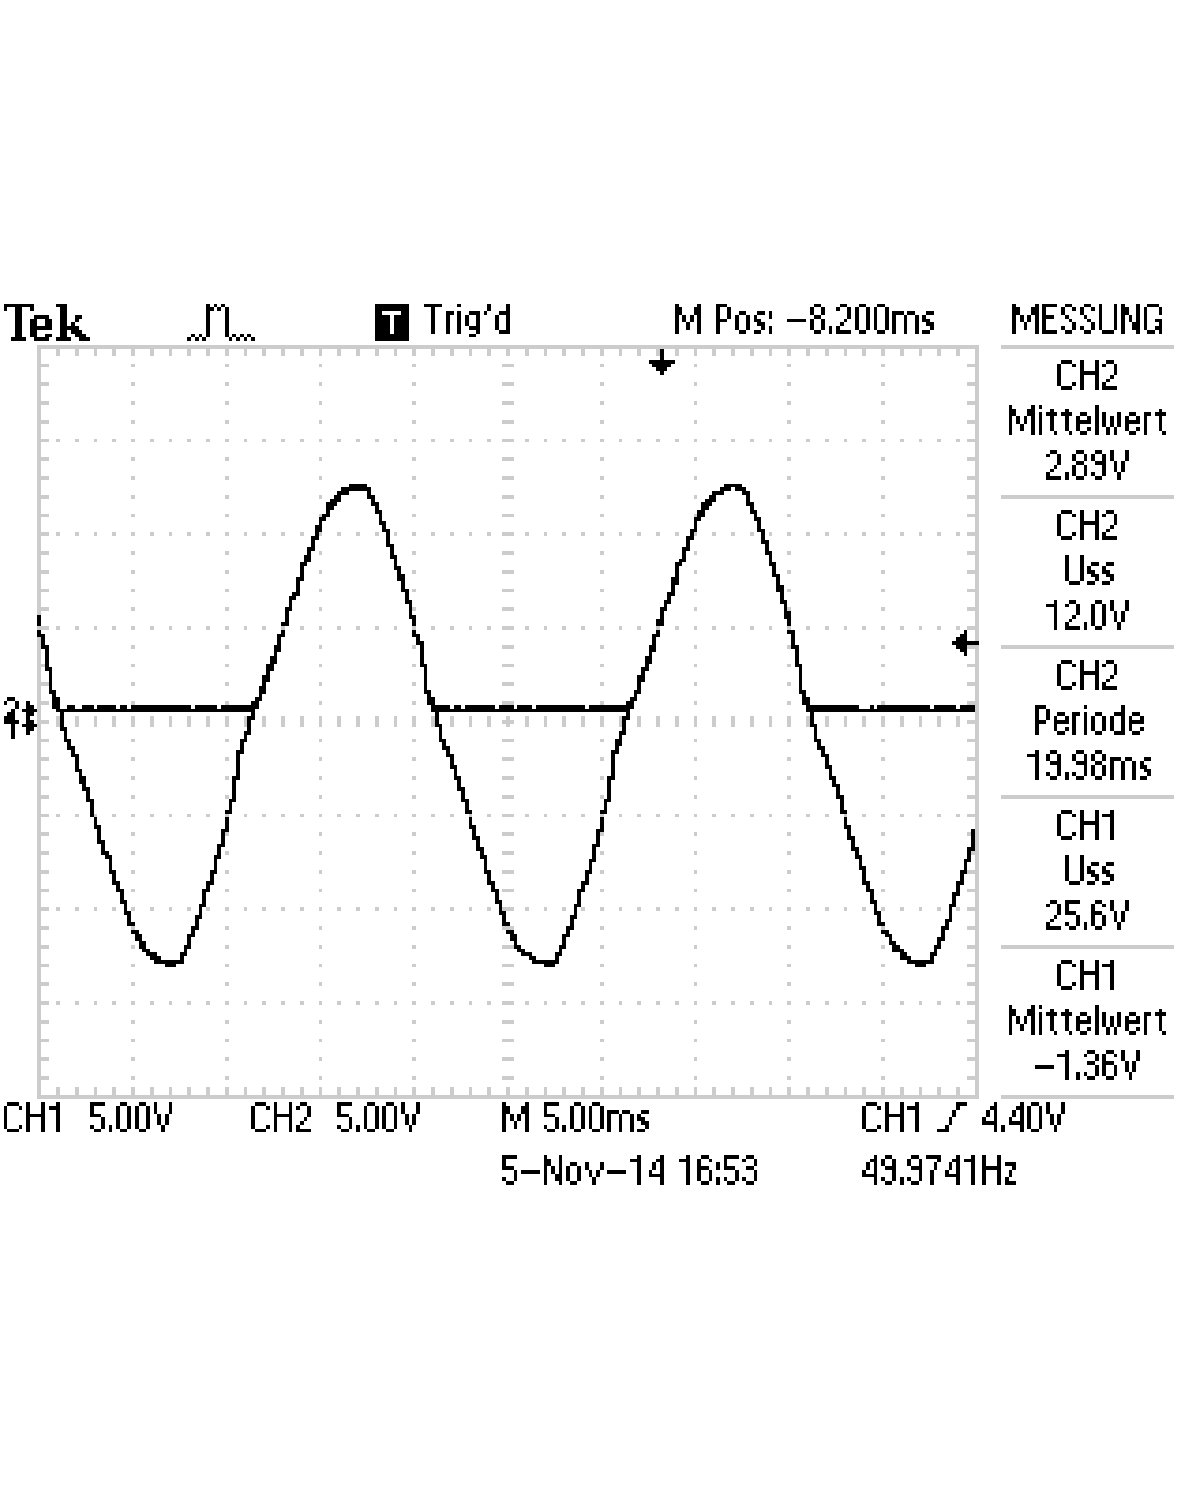
\includegraphics[width=\textwidth , scale = 0.4]{2_3_1.pdf}
                \caption[Aufnahme bei maximalem Widerstand]{Aufnahme bei maximalem Widerstand}
 				 \label{fig:2_3_1}
        \end{subfigure}%
        %~ %add desired spacing between images, e. g. ~, \quad, \qquad, \hfill etc.
          %(or a blank line to force the subfigure onto a new line)
        \hfill
        \begin{subfigure}[b]{0.48\textwidth}
                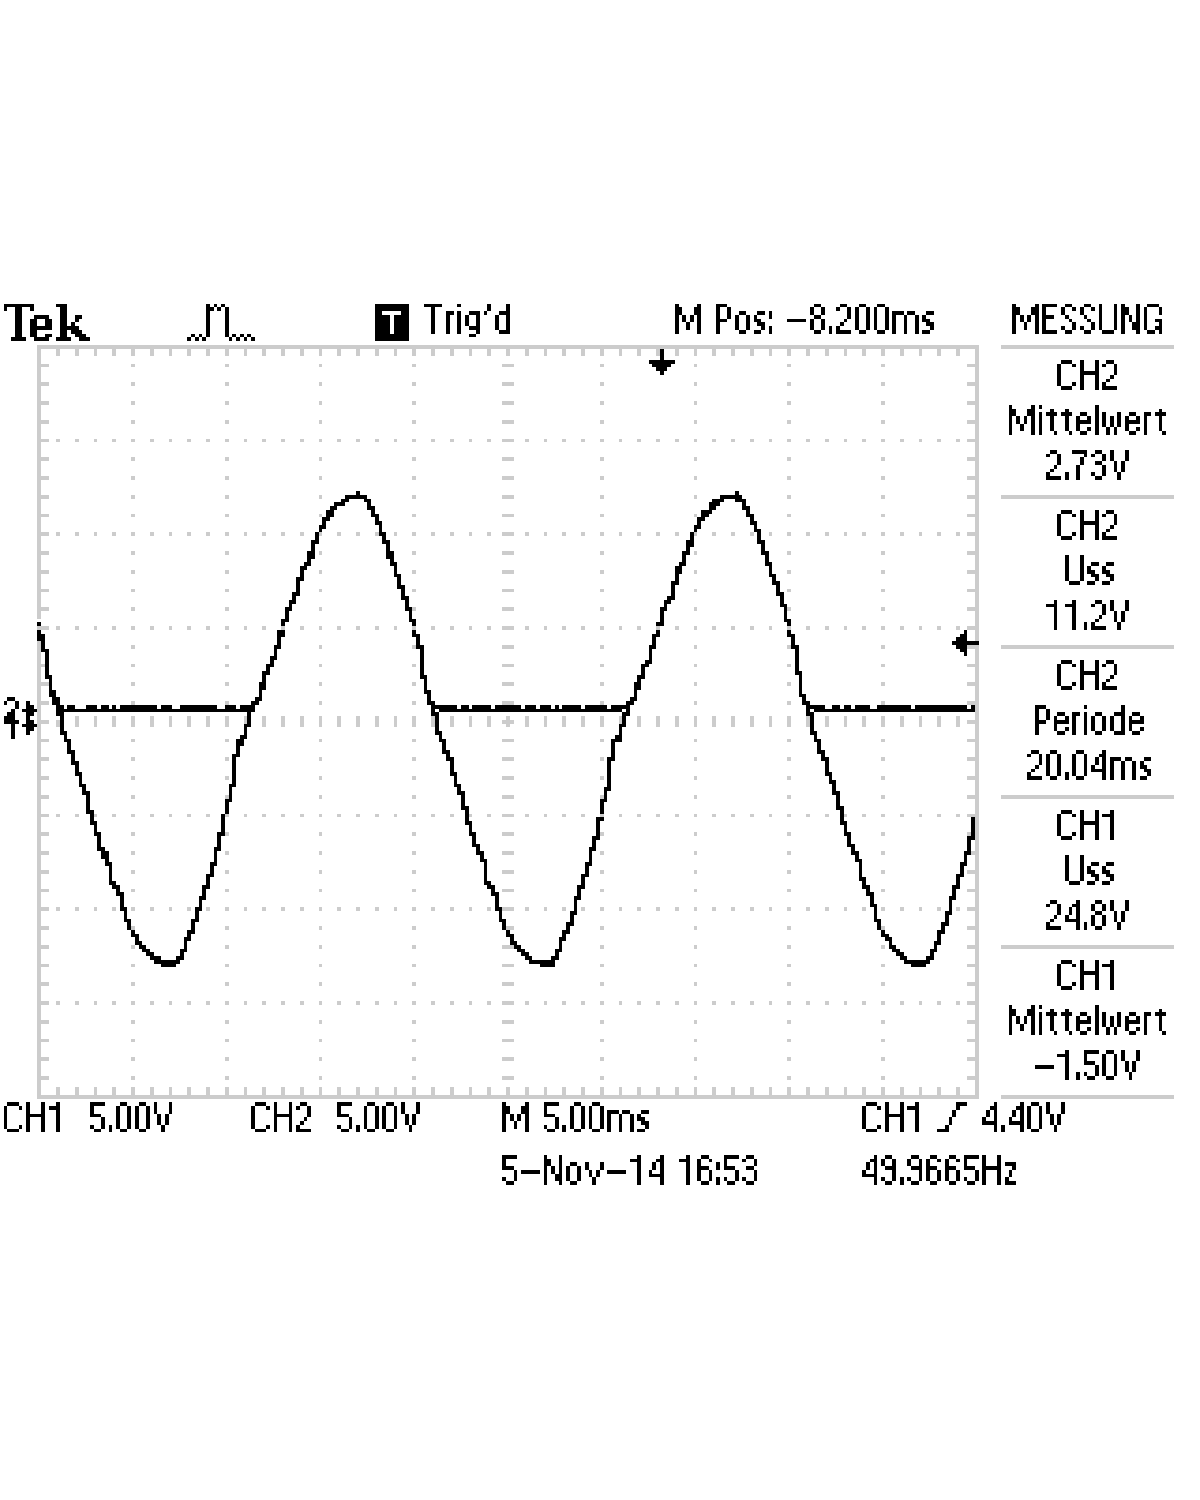
\includegraphics[width=\textwidth , scale = 0.4]{2_3_2.pdf}
                \caption[Aufnahme bei minimalem Widerstand]{Aufnahme bei minimalem Widerstand}
  				\label{fig:2_3_2}
        \end{subfigure}
        \caption{Aufnahme der Ausgangsspannung bei minimalem und maximalem Widerstand}
        \label{fig:2_3}
\end{figure}


\subsection{Einweggleichrichtung mit Kondensator}
Die durch den Transformator erzeugte Wechselspannung soll wie im vorletzten Versuchsteil gleichgerichtet werden.
\subsubsection{Versuchsaufbau}
%skizze zum versuchsaufbau (oder foto) einfügen,   es muss erklärt werden wie das ganze funktioniert und welche speziellen einstellungen verwendet wurden (z.b. welche knöpfe an den geräten für die messung verdreht wurden)
Es wird der selbe Versuchsaufbau wie in Abbildung \ref{fig:2_4} verwendet, mit einem zwischen Elektrolytkondensator, der Parallel zum Potentiometer und der Glühlampe geschaltet ist. Der Elektrolytkondensator wird hinter der Diode eingebaut. Es wird ein Elektrolytkondensator mit 100$\mu$F oder 1000$\mu$F verwendet.

\begin{figure}[H] 
  \centering
    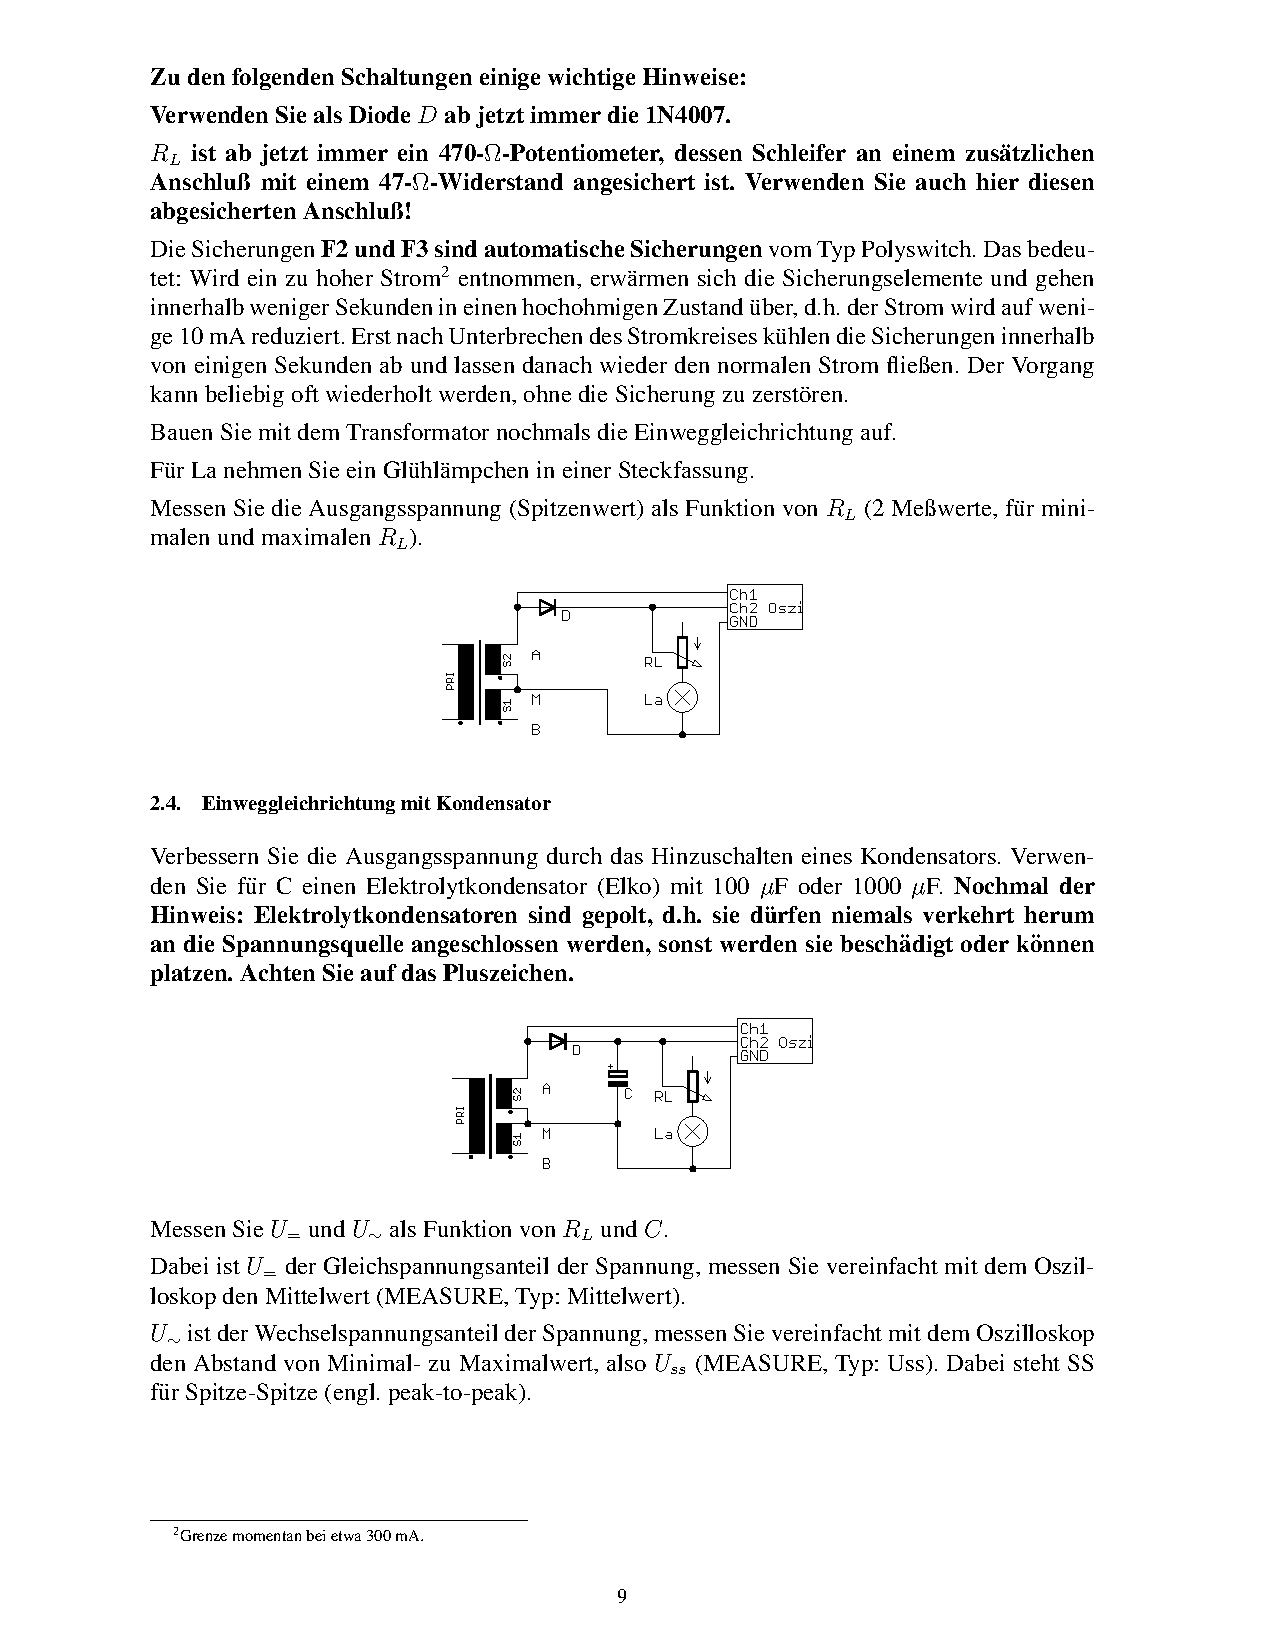
\includegraphics[trim = 10mm 80mm 10mm 170mm, clip, scale = 1]{ep2_14[Page9].pdf}
  	\caption[Schaltskizze der Einweggleichrichtung mit Transformator]{Schaltskizze der Einweggleichrichtung mit Transformator\footnotemark}
  \label{fig:2_5}
\end{figure}
\footnotetext{Abbildung entnommen von http://www.atlas.uni-wuppertal.de/$\sim$kind/ep2\_14.pdf Seite 9 am 28.10.2014}

\subsubsection{Versuchsdurchführung}
%erklären, !was! wir machen, !warum! wir das machen und mit welchem ziel
%(wichtig) präzize erklären, wie bei dem versuch vorgegangen und was gemacht wurde
Vergleichbar mit dem zweiten Teil werden nun Kondensatoren (1000 und \unit[100]{$\mu$F}) parallel zur Last geschaltet, um den starken Spannungsabfall entgegen der Durchlassrichtung zu verhindern \footnote{Versuchsaufbau: Abb. \ref{fig:2_5}}. Am Oszilloskop wird Wechsel- und Gleichspannungsanteil angezeigt, wobei der Potentiometerwiderstand zum Einen maximal (\unit[517]{$\Omega$} und zum Anderen minimal gewählt wird.
\subsubsection{Auswertung}
%zuerst !alle! errechneten werte entweder in ganzen sätzen aufzählen, oder in tabellen (übersichtlicher) dargestellen, sowie auf die verwendeten formeln verweisen (die referenzierung der formel kann in der überschrift stehen)
%kurz erwähnen (vor der tabelle), warum wir das ganze ausrechnen bzw. was wir dort ausrechnen
%danach histogramme und plots erstellen, wobei wenn möglich funktionen durch die plots gelegt werden (zur not können auch splines benutzt werden, was aber angegeben werden muss)
%bei fits immer die funktion und das reduzierte chiquadrat mit angegeben, wobei auf verständlichkeit beim entziffern der zehnerpotenzen geachtet werden muss z.b. f(x)=(wert+-fehler)\cdot10^{irgendeine zahl}\cdot x + (wert+-fehler)\cdot10^{irgendeine zahl}
%bei jedem fit erklären, nach welchem zusammenhang gefittet wurde und warum!
%bei plots darauf achten, dass die achsenbeschriftung (auch die tics) die richtige größe haben und die legende im plot nicht die messwerte verdeckt
%kurz die aufgabenstellung abgehandeln

In diesem Versuchsteil soll der Gleichspannungs- und der Wechselspannungsanteil, des ankommenden Signals gemessen werden. Diese Messung wurde einmal für minimales und für maximales RL durchgeführt. Es wurde Messungen für 100$\mu$F und 1000$\mu$F vorgenommen. Für den 100$\mu$F Kondensator ergaben sich die Verläufe aus Abbildung \ref{fig:2_4_100F}.

\begin{figure}[H]
        \centering
        \begin{subfigure}[b]{0.48\textwidth}
                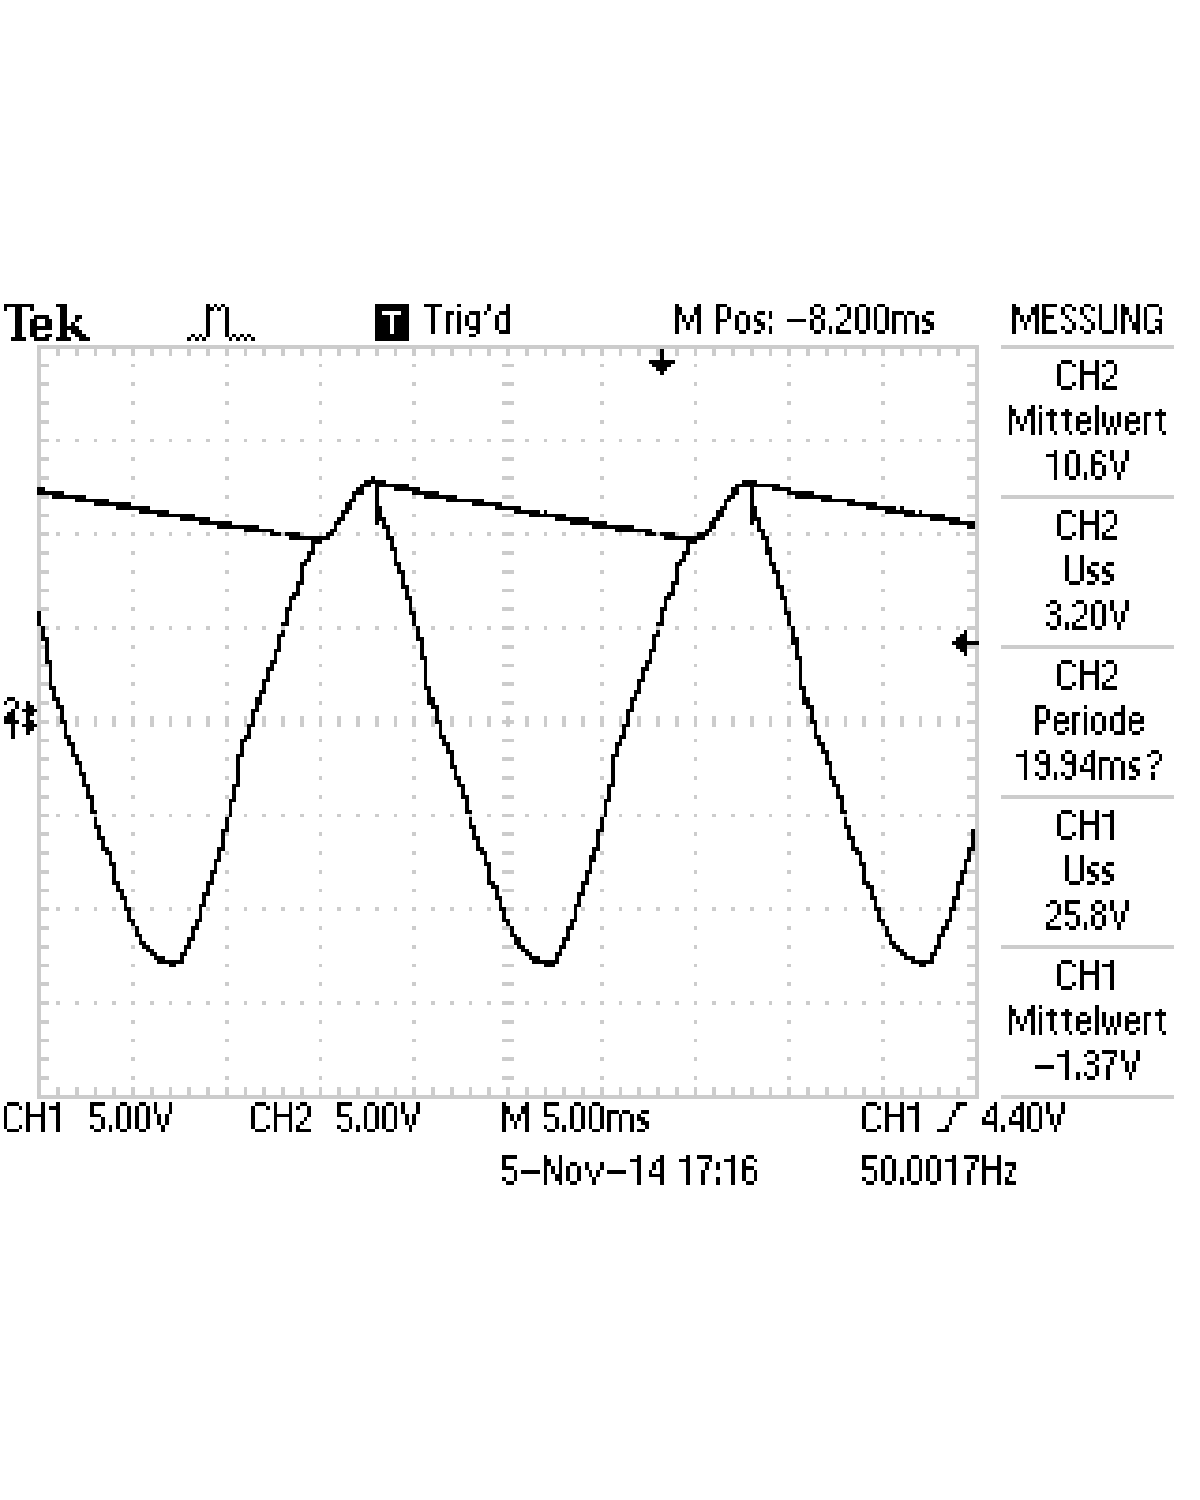
\includegraphics[width=\textwidth , scale = 0.4]{2_4_100F_1.pdf}
                \caption[Aufnahme bei maximalem Widerstand. U$_{=}$ = 10,6V und U$_\sim$ = 3,20V]{Aufnahme bei maximalem Widerstand. U$_{=}$ = 10,6V und U$_\sim$ = 3,20V}
 				 \label{fig:2_4_100F_1}
        \end{subfigure}%
        %~ %add desired spacing between images, e. g. ~, \quad, \qquad, \hfill etc.
          %(or a blank line to force the subfigure onto a new line)
        \hfill
        \begin{subfigure}[b]{0.48\textwidth}
                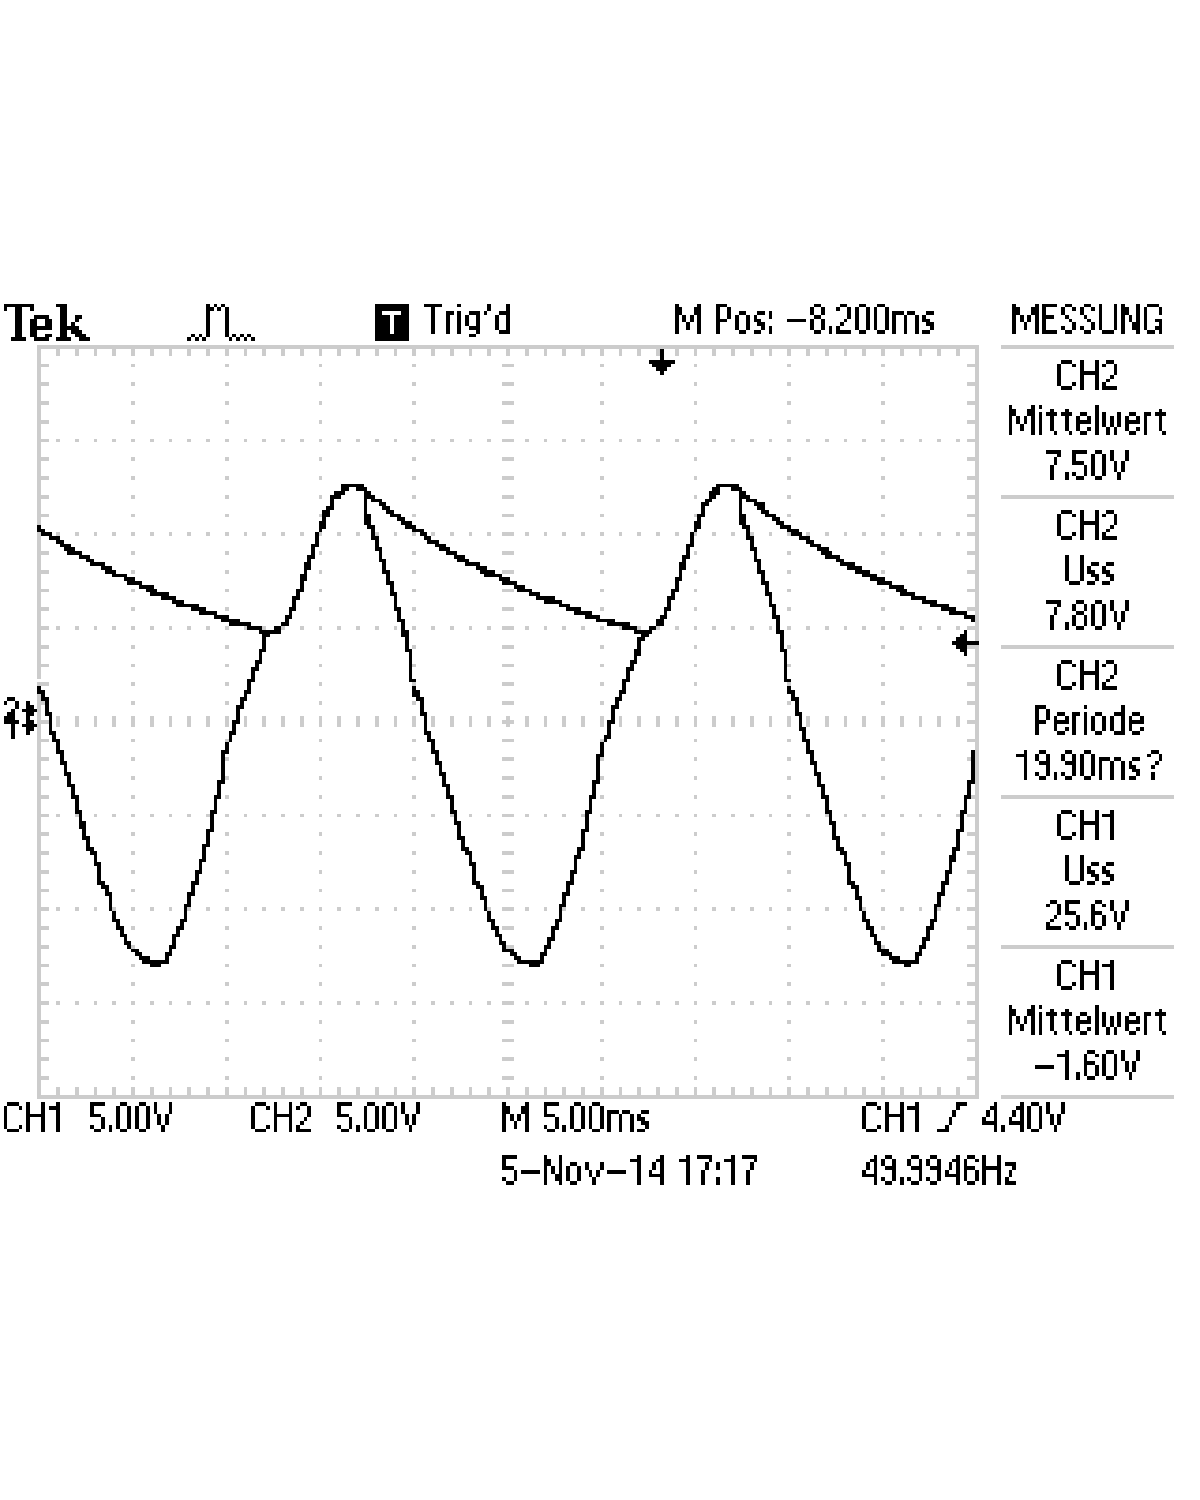
\includegraphics[width=\textwidth , scale = 0.4]{2_4_100F_2.pdf}
                \caption[Aufnahme bei minimalem Widerstand. U$_{=}$ = 7,5V und U$_\sim$ = 7,80V]{Aufnahme bei minimalem Widerstand. U$_{=}$ = 7,5V und U$_\sim$ = 7,80V}
  				\label{fig:2_4_100F_2}
        \end{subfigure}
        \caption{Aufnahme der Ausgangsspannung bei minimalem und maximalem Widerstand}
        \label{fig:2_4_100F}
\end{figure}

Für den 1000$\mu$F Kondensator ergaben sich die Verläufe in Abbildung \ref{fig:2_4_1000F}.

\begin{figure}[H]
        \centering
        \begin{subfigure}[b]{0.48\textwidth}
                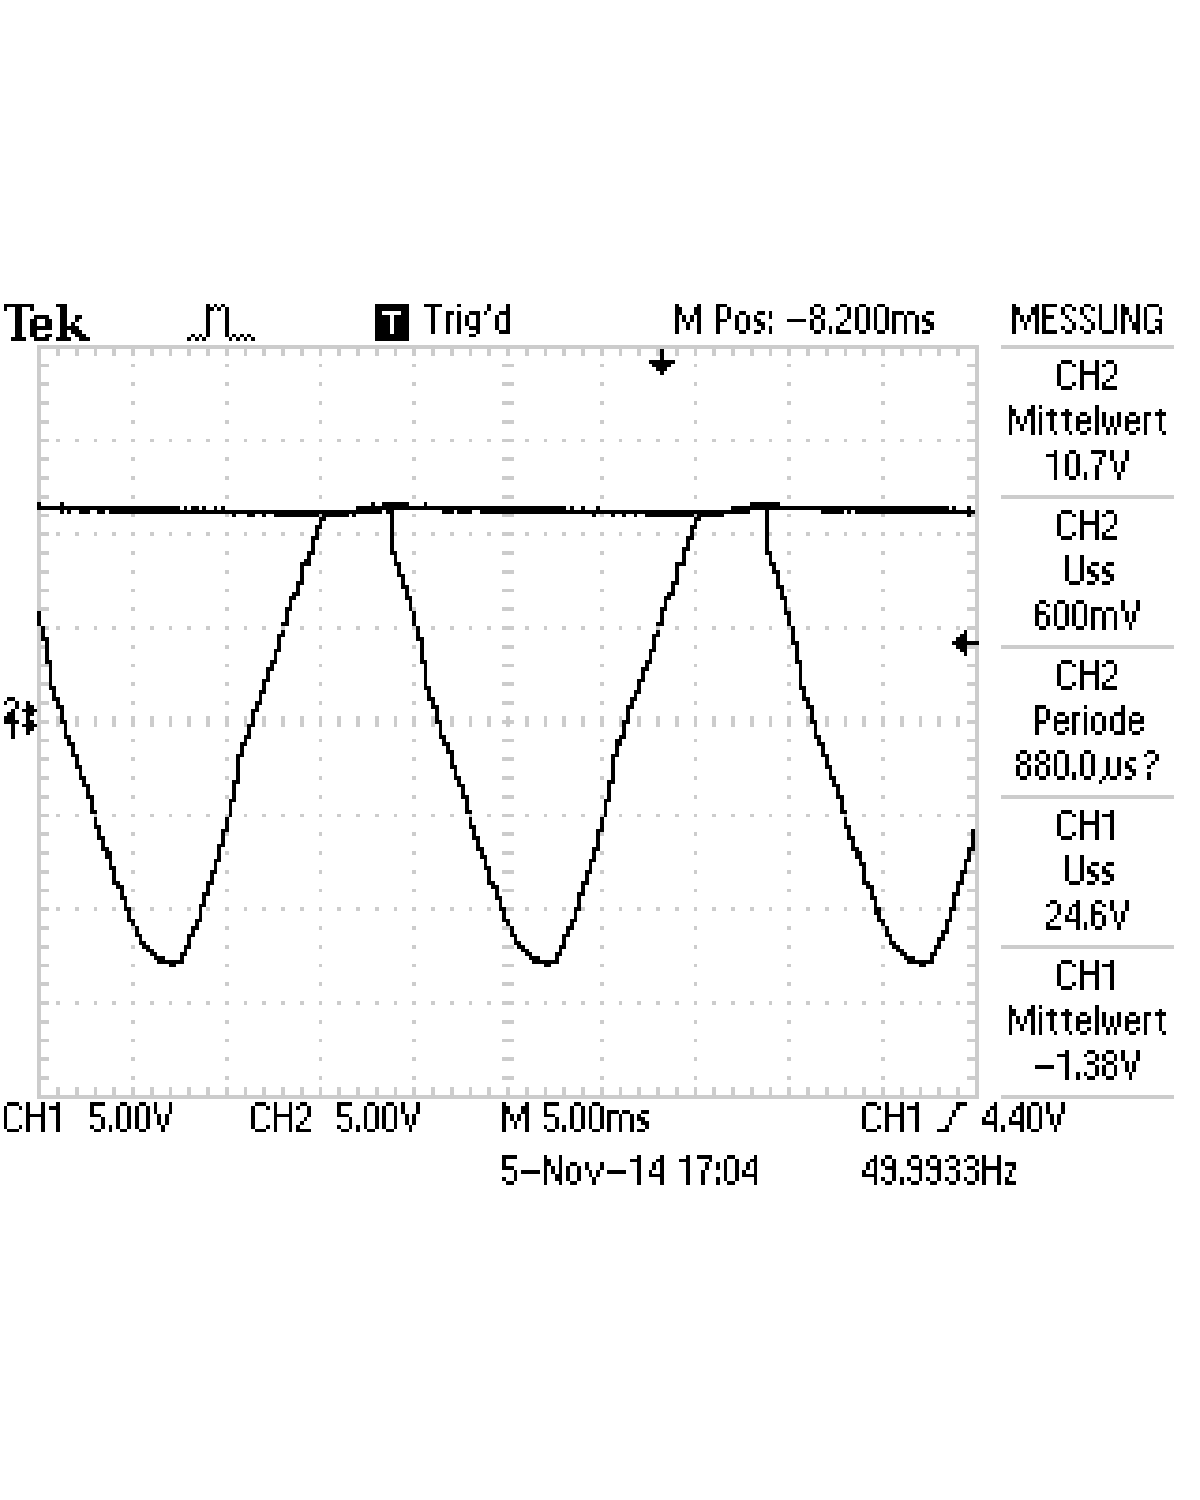
\includegraphics[width=\textwidth , scale = 0.4]{2_4_1000F_1.pdf}
                \caption[Aufnahme bei maximalem Widerstand. U$_{=}$ = 10,7V und U$_\sim$ = 0,6V]{Aufnahme bei maximalem Widerstand. U$_{=}$ = 10,7V und U$_\sim$ = 0,6Vd}
 				 \label{fig:2_4_1000F_1}
        \end{subfigure}%
        %~ %add desired spacing between images, e. g. ~, \quad, \qquad, \hfill etc.
          %(or a blank line to force the subfigure onto a new line)
        \hfill
        \begin{subfigure}[b]{0.48\textwidth}
                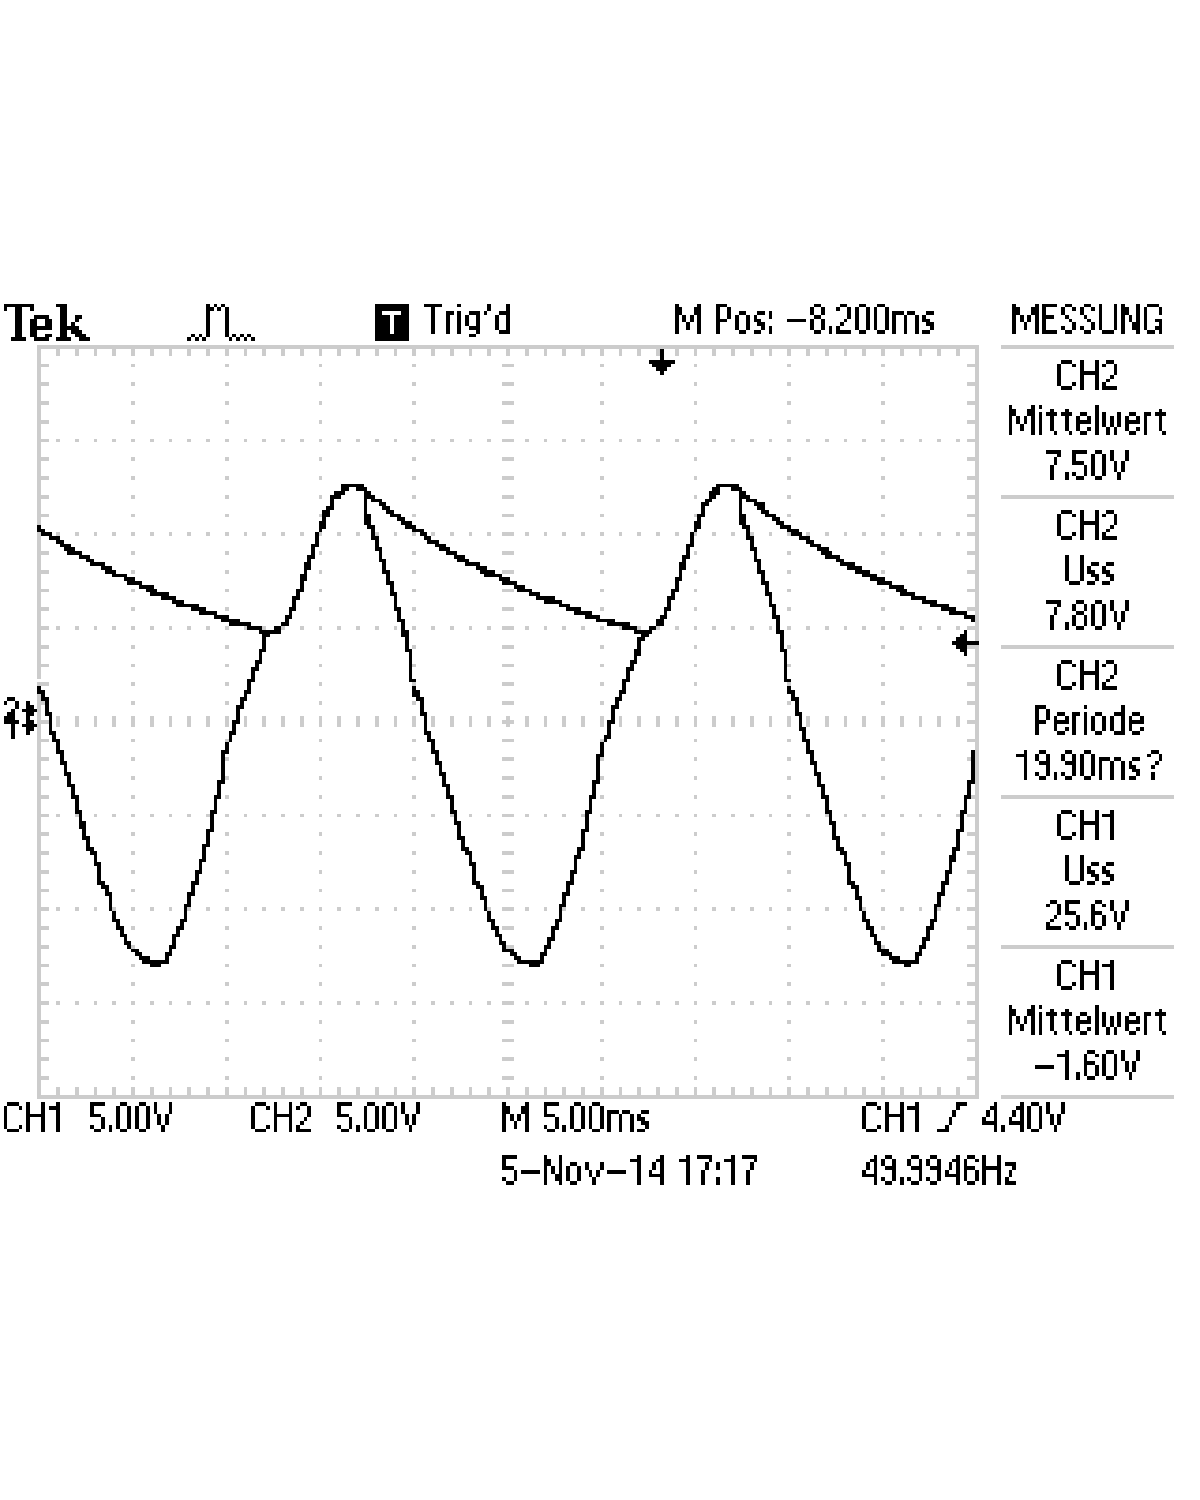
\includegraphics[width=\textwidth , scale = 0.4]{2_4_100F_2.pdf}
                \caption[Aufnahme bei minimalem Widerstand. U$_{=}$ = 7,5V und U$_\sim$ = 7,8V]{Aufnahme bei minimalem Widerstand. U$_{=}$ = 7,5V und U$_\sim$ = 7,8V}
  				\label{fig:2_4_1000F_2}
        \end{subfigure}
        \caption{Aufnahme der Ausgangsspannung bei minimalem und maximalem Widerstand}
        \label{fig:2_4_1000F}
\end{figure}

\subsection{Doppelweggleichrichtung mit Kondensator}

Durch eine zweite Diode am unterem Teil des Transformators wir aus dem Einwegrichter ein Doppelwegrichter gebaut, sodass sich die Spannungen ergänzten.

\subsubsection{Versuchsaufbau}
%skizze zum versuchsaufbau (oder foto) einfügen,   es muss erklärt werden wie das ganze funktioniert und welche speziellen einstellungen verwendet wurden (z.b. welche knöpfe an den geräten für die messung verdreht wurden)
Es werden Elektrolytkondensatoren mit 100$\mu$F oder 1000$\mu$F verwendet. R$_\text{L}$ ist ein 470$\Omega$ Potentiometer und La eine Glühlampe. Als Dioden werden wieder 1N4007 Dioden verwendet.

\begin{figure}[H] 
  \centering
    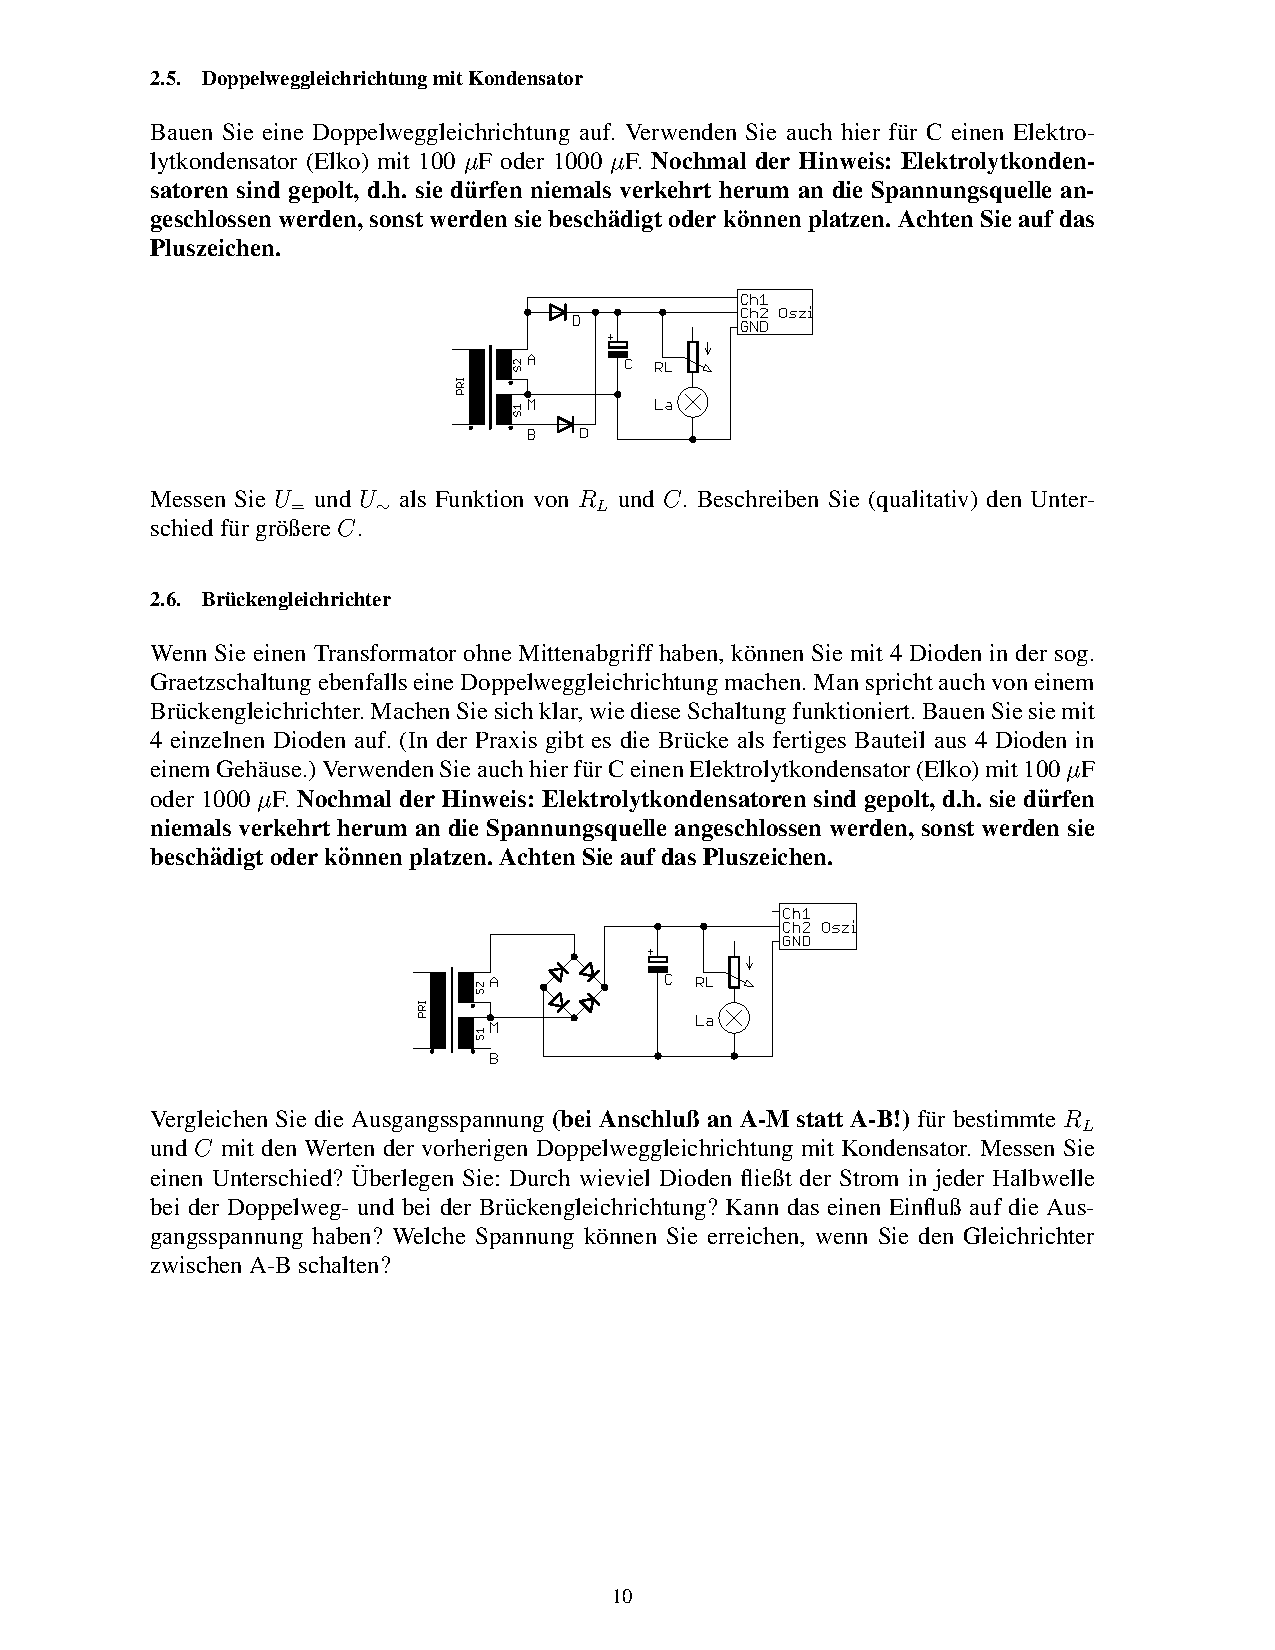
\includegraphics[trim = 10mm 200mm 10mm 45mm, clip, scale = 1]{ep2_14[Page10].pdf}
  	\caption[Schaltskizze der Einweggleichrichtung mit Transformator]{Schaltskizze der Einweggleichrichtung mit Transformator\footnotemark}
  \label{fig:2_6}
\end{figure}
\footnotetext{Abbildung entnommen von http://www.atlas.uni-wuppertal.de/$\sim$kind/ep2\_14.pdf Seite 10 am 28.10.2014}

\subsubsection{Versuchsdurchführung}
%erklären, !was! wir machen, !warum! wir das machen und mit welchem ziel
%(wichtig) präzize erklären, wie bei dem versuch vorgegangen und was gemacht wurde
Nun wird am unteren Ende des Trafos eine Diode dazugeschaltet \footnote{Versuchsaufbau: Abb. \ref{fig:2_6}}, welche mit einer um \unit[180]{Grad} verschobenen Spannung betrieben wird, sodass sich die von beiden Dioden durchgalassenen Spannungen ergänzen. Bei minimalem und maximalem Potentiometerwiderstand sowie bei Kapazitäten von 1000 und \unit[100]{$\mu$F} werden die Messungen wiederholt und mit den Versuchsteilen davor verglichen.
\subsubsection{Auswertung}
%zuerst !alle! errechneten werte entweder in ganzen sätzen aufzählen, oder in tabellen (übersichtlicher) dargestellen, sowie auf die verwendeten formeln verweisen (die referenzierung der formel kann in der überschrift stehen)
%kurz erwähnen (vor der tabelle), warum wir das ganze ausrechnen bzw. was wir dort ausrechnen
%danach histogramme und plots erstellen, wobei wenn möglich funktionen durch die plots gelegt werden (zur not können auch splines benutzt werden, was aber angegeben werden muss)
%bei fits immer die funktion und das reduzierte chiquadrat mit angegeben, wobei auf verständlichkeit beim entziffern der zehnerpotenzen geachtet werden muss z.b. f(x)=(wert+-fehler)\cdot10^{irgendeine zahl}\cdot x + (wert+-fehler)\cdot10^{irgendeine zahl}
%bei jedem fit erklären, nach welchem zusammenhang gefittet wurde und warum!
%bei plots darauf achten, dass die achsenbeschriftung (auch die tics) die richtige größe haben und die legende im plot nicht die messwerte verdeckt
%kurz die aufgabenstellung abgehandeln

In diesem Versuchsteil soll der Gleichspannungs- und der Wechselspannungsanteil, des ankommenden Signals gemessen werden. Diese Messung wurde einmal für minimales und für maximales RL durchgeführt. Es wurde Messungen für 100$\mu$F und 1000$\mu$F vorgenommen. Für den 100$\mu$F Kondensator ergaben sich die Verläufe aus Abbildung \ref{fig:2_5_100F}.

\begin{figure}[H]
        \centering
        \begin{subfigure}[b]{0.48\textwidth}
                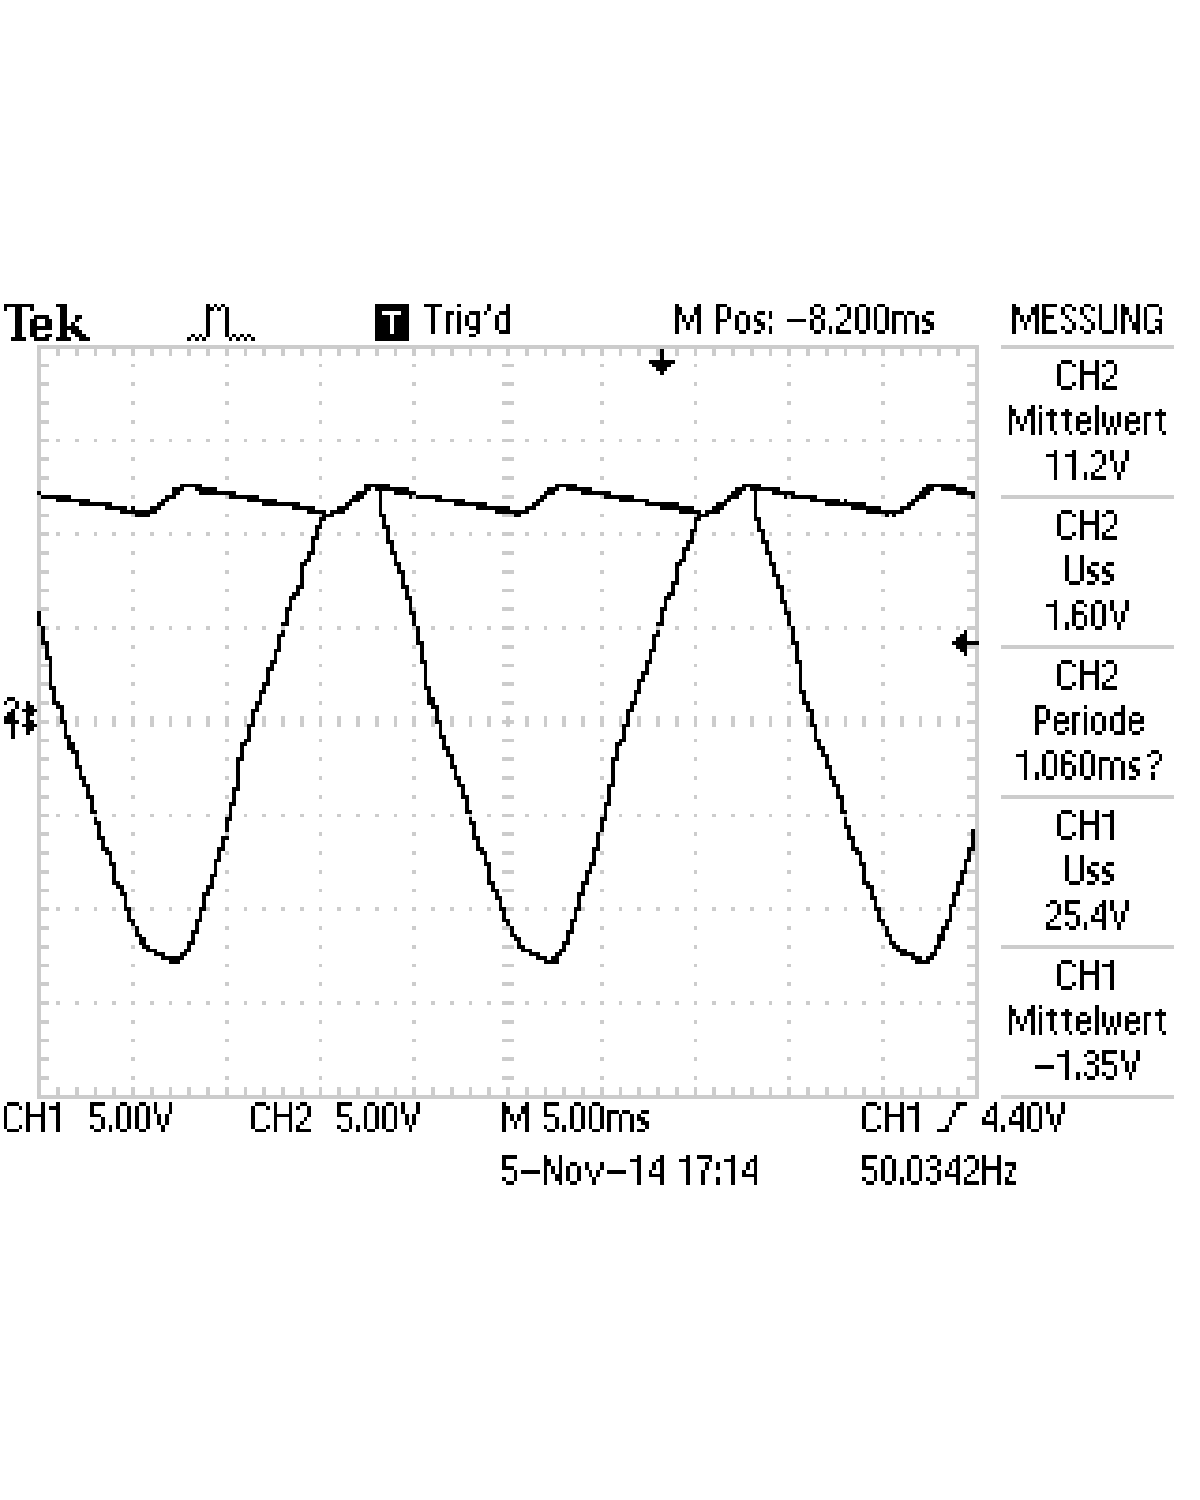
\includegraphics[width=\textwidth , scale = 0.4]{2_5_100F_1.pdf}
                \caption[Aufnahme bei maximalem Widerstand. U$_{=}$ = 11,2V und U$_\sim$ = 1,6V]{Aufnahme bei maximalem Widerstand. U$_{=}$ = 11,2V und U$_\sim$ = 1,6V}
 				 \label{fig:2_5_100F_1}
        \end{subfigure}%
        %~ %add desired spacing between images, e. g. ~, \quad, \qquad, \hfill etc.
          %(or a blank line to force the subfigure onto a new line)
        \hfill
        \begin{subfigure}[b]{0.48\textwidth}
                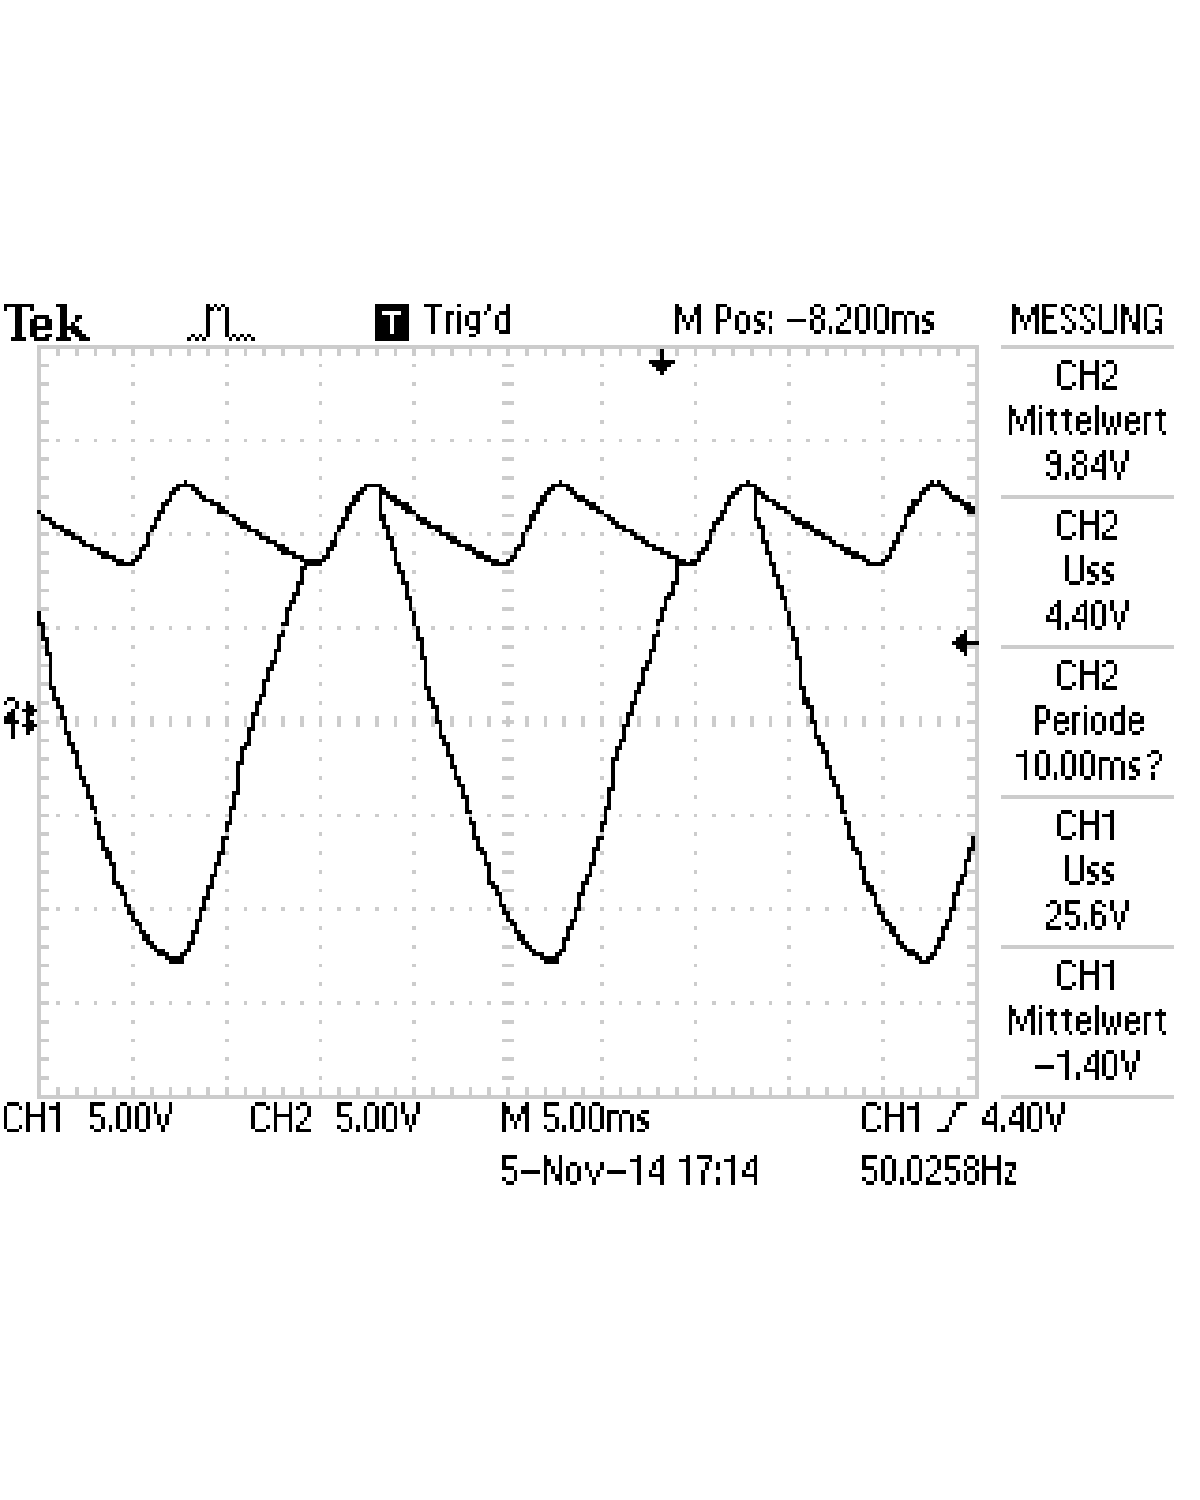
\includegraphics[width=\textwidth , scale = 0.4]{2_5_100F_2.pdf}
                \caption[Aufnahme bei minimalem Widerstand. U$_{=}$ = 9,84V und U$_\sim$ = 4,4V]{Aufnahme bei minimalem Widerstand. U$_{=}$ = 9,84V und U$_\sim$ = 4,4V}
  				\label{fig:2_5_100F_2}
        \end{subfigure}
        \caption{Aufnahme der Ausgangsspannung bei minimalem und maximalem Widerstand}
        \label{fig:2_5_100F}
\end{figure}

Für den 1000$\mu$F Kondensator ergaben sich die Verläufe in Abbildung \ref{fig:2_5_1000F}.

\begin{figure}[H]
        \centering
        \begin{subfigure}[b]{0.48\textwidth}
                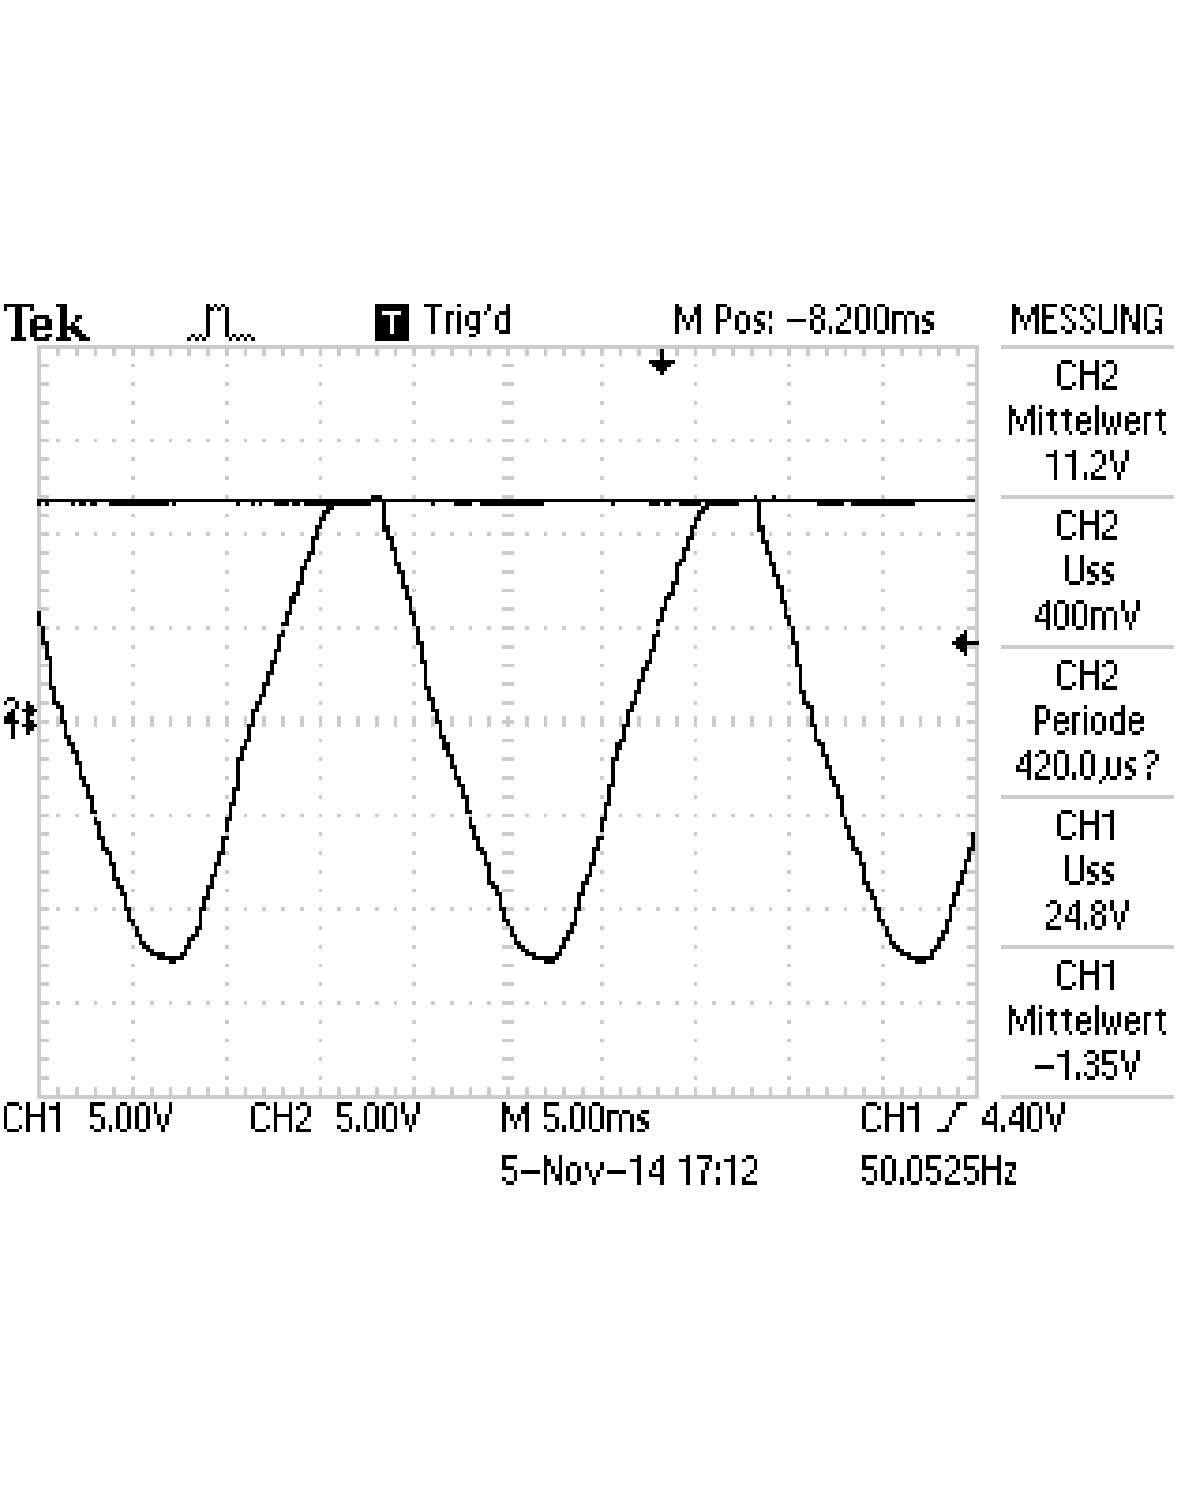
\includegraphics[width=\textwidth , scale = 0.4]{2_5_1000F_1.pdf}
                \caption[Aufnahme bei maximalem Widerstand. U$_{=}$ = 11,2V und U$_\sim$ = 0,4V]{Aufnahme bei maximalem Widerstand. U$_{=}$ = 11,2V und U$_\sim$ = 0,4V}
 				 \label{fig:2_5_1000F_1}
        \end{subfigure}%
        %~ %add desired spacing between images, e. g. ~, \quad, \qquad, \hfill etc.
          %(or a blank line to force the subfigure onto a new line)
        \hfill
        \begin{subfigure}[b]{0.48\textwidth}
                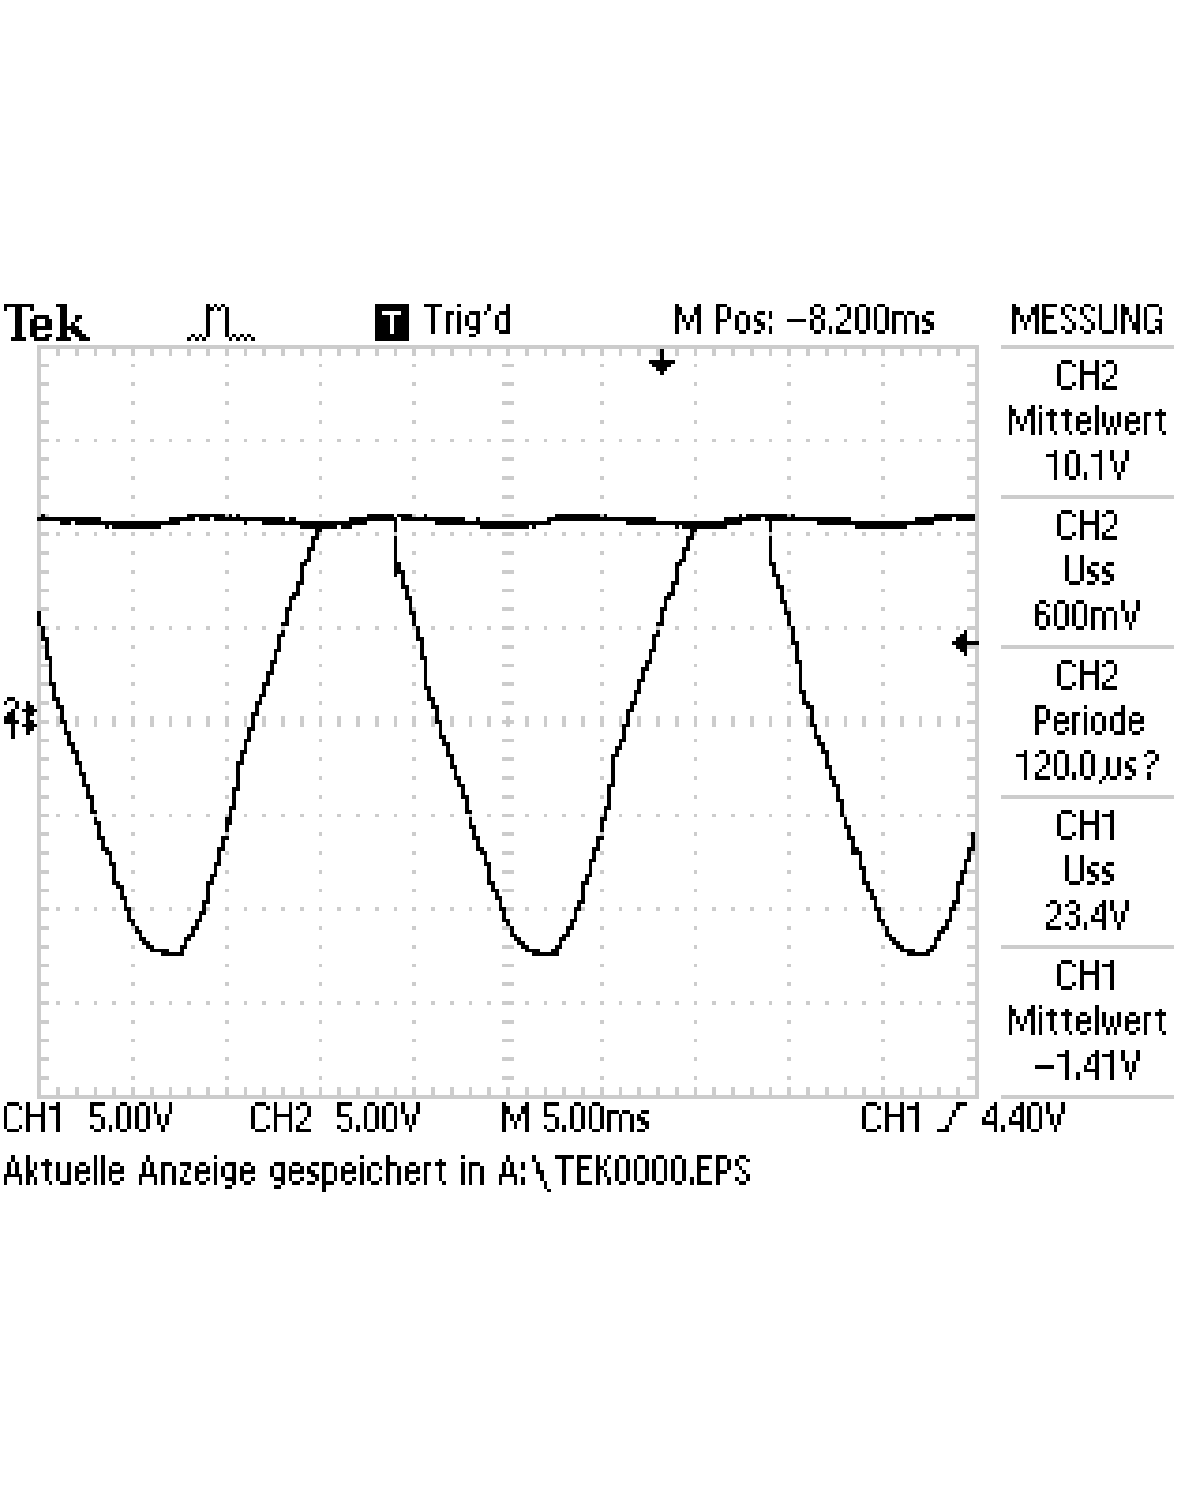
\includegraphics[width=\textwidth , scale = 0.4]{2_5_1000F_2.pdf}
                \caption[Aufnahme bei minimalem Widerstand. U$_{=}$ = 10,1V und U$_\sim$ = 0,6V]{Aufnahme bei minimalem Widerstand. U$_{=}$ = 10,1V und U$_\sim$ = 0,6V}
  				\label{fig:2_5_1000F_2}
        \end{subfigure}
        \caption{Aufnahme der Ausgangsspannung bei minimalem und maximalem Widerstand}
        \label{fig:2_5_1000F}
\end{figure}

Bei hohem Widerstand wird bei dem Kondensator mit größerer Kapazität ein höherer Gleichspannungsanteil erreicht.

\subsection{Brückengleichrichter}
Ein aus vier Dioden bestehender Brückengleichrichter wird an den Transformator angeschlossen. Ähnlich wie im Versuchsteil davor ergänzen sich positive und negative Spannung.
\subsubsection{Versuchsaufbau}
%skizze zum versuchsaufbau (oder foto) einfügen,   es muss erklärt werden wie das ganze funktioniert und welche speziellen einstellungen verwendet wurden (z.b. welche knöpfe an den geräten für die messung verdreht wurden)
Als Elektrolytkondensator wird wieder einer mit 100$\mu$F oder 1000$\mu$F verwendet. Bei den Dioden handelt es sich wider um 1N4007 Dioden. RL ist ein 470$\Omega$ Potentiometer und La ist eine Glühlampe.
\begin{figure}[H] 
  \centering
    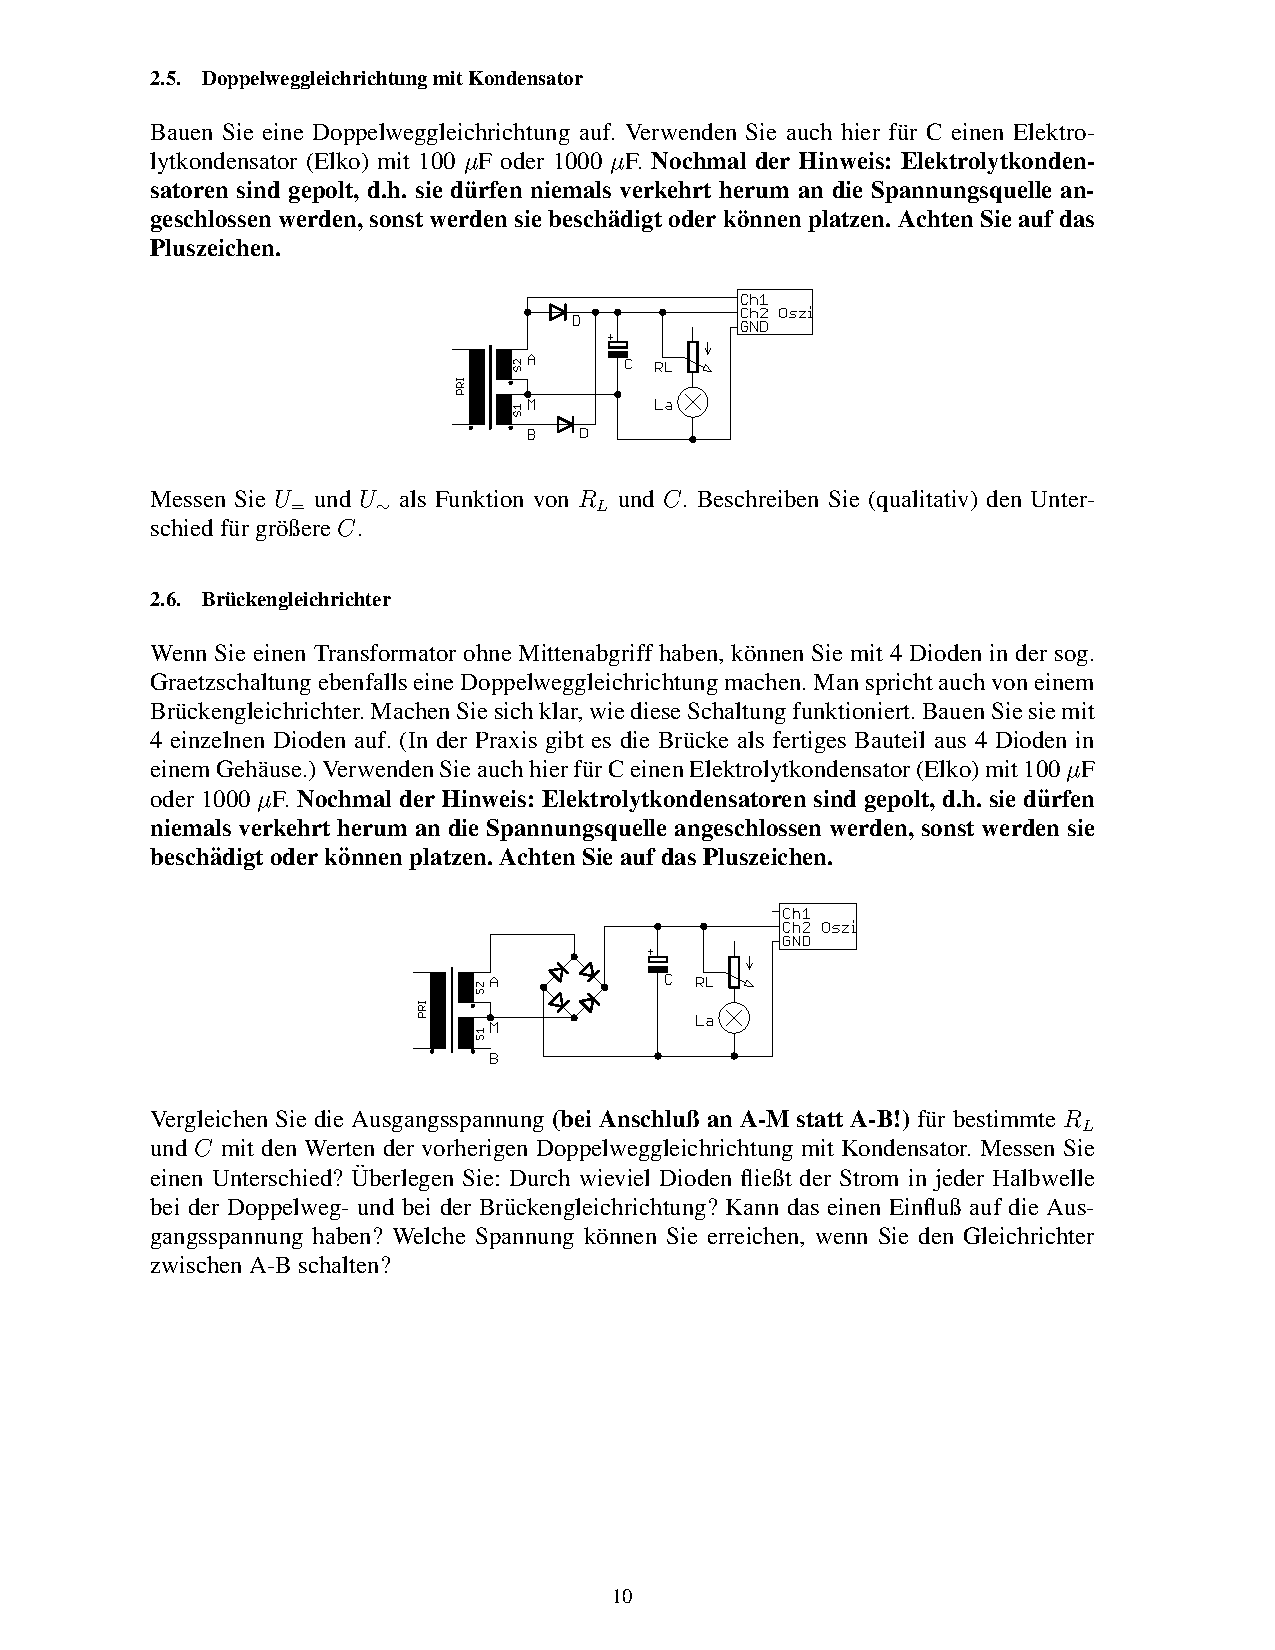
\includegraphics[trim = 10mm 100mm 10mm 150mm, clip, scale = 1]{ep2_14[Page10].pdf}
  	\caption[Schaltskizze für einen Brückengleichrichter]{Schaltskizze für einen Brückengleichrichter\footnotemark}
  \label{fig:2_7}
\end{figure}
\footnotetext{Abbildung entnommen von http://www.atlas.uni-wuppertal.de/$\sim$kind/ep2\_14.pdf Seite 10 am 28.10.2014}

\subsubsection{Versuchsdurchführung}
%erklären, !was! wir machen, !warum! wir das machen und mit welchem ziel
%(wichtig) präzize erklären, wie bei dem versuch vorgegangen und was gemacht wurde
Zuletzt werden die zwei Dioden aus dem Versuchsteil davor durch 4 Dioden in einer Brückengleichrichterschaltung ersetzt \footnote{Versuchsaufbau: Abb. \ref{fig:2_7}}. Dies hat den Vorteil einer "gleichmäßigeren" Gleichspannung und den Nachteil einer doppelten Anregespannung für die Dioden. Die Messungen werden Analog zu den Versuchsteilen davor für Kapazitäten von 1000 und \unit[100]{$\mu$F} durchgeführt sowie miteinander verglichen.
\subsubsection{Auswertung}
%zuerst !alle! errechneten werte entweder in ganzen sätzen aufzählen, oder in tabellen (übersichtlicher) dargestellen, sowie auf die verwendeten formeln verweisen (die referenzierung der formel kann in der überschrift stehen)
%kurz erwähnen (vor der tabelle), warum wir das ganze ausrechnen bzw. was wir dort ausrechnen
%danach histogramme und plots erstellen, wobei wenn möglich funktionen durch die plots gelegt werden (zur not können auch splines benutzt werden, was aber angegeben werden muss)
%bei fits immer die funktion und das reduzierte chiquadrat mit angegeben, wobei auf verständlichkeit beim entziffern der zehnerpotenzen geachtet werden muss z.b. f(x)=(wert+-fehler)\cdot10^{irgendeine zahl}\cdot x + (wert+-fehler)\cdot10^{irgendeine zahl}
%bei jedem fit erklären, nach welchem zusammenhang gefittet wurde und warum!
%bei plots darauf achten, dass die achsenbeschriftung (auch die tics) die richtige größe haben und die legende im plot nicht die messwerte verdeckt
%kurz die aufgabenstellung abgehandeln
In diesem Aufgabenteil sollte die Ausgangsspannung in Abhängigkeit der Kapazität des Kondensator und des Widerstandes des Kondensators gemessen werden. Als Kapazitäten wurden 100$\mu$F und 1000$\mu$F verwendet. Dabei ergab sich bei dem 100$\mu$F Kondensator die Verläufe in Abbildung \ref{fig:2_6_100F}.

\begin{figure}[H]
        \centering
        \begin{subfigure}[b]{0.48\textwidth}
                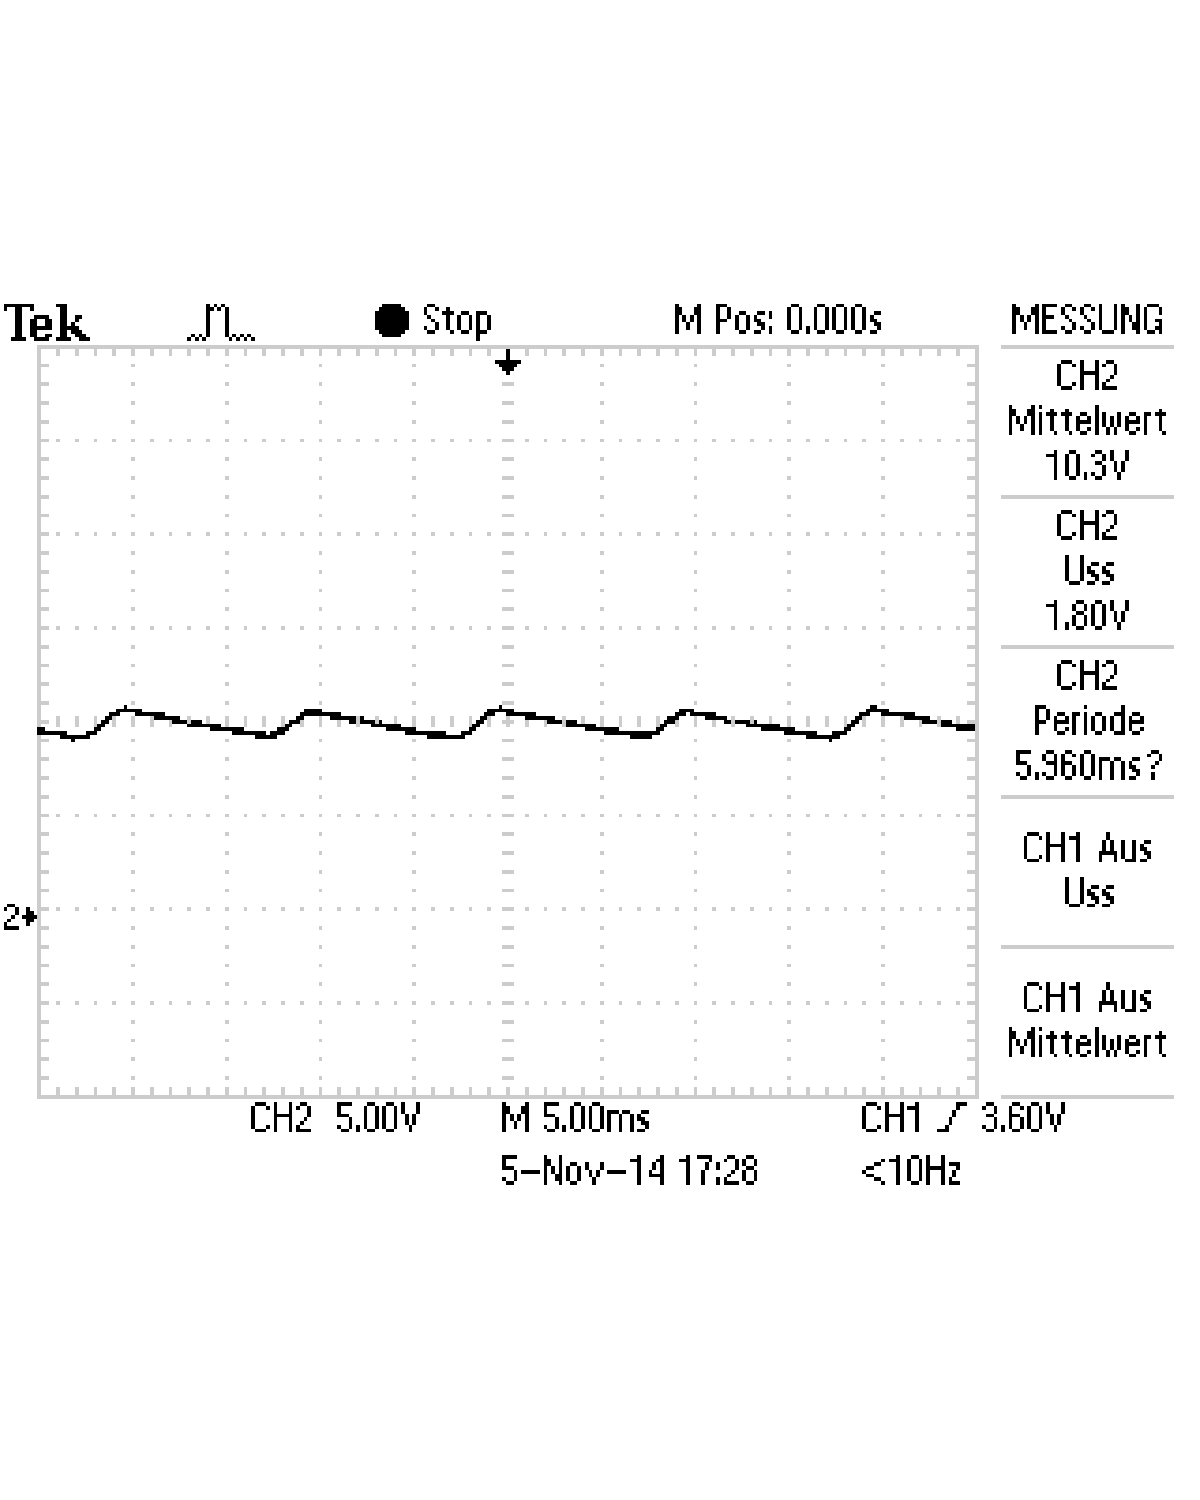
\includegraphics[width=\textwidth , scale = 0.4]{2_6_100F_1.pdf}
                \caption[Aufnahme bei maximalem Widerstand]{Aufnahme bei maximalem Widerstand}
 				 \label{fig:2_6_100F_1}
        \end{subfigure}%
        %~ %add desired spacing between images, e. g. ~, \quad, \qquad, \hfill etc.
          %(or a blank line to force the subfigure onto a new line)
        \hfill
        \begin{subfigure}[b]{0.48\textwidth}
                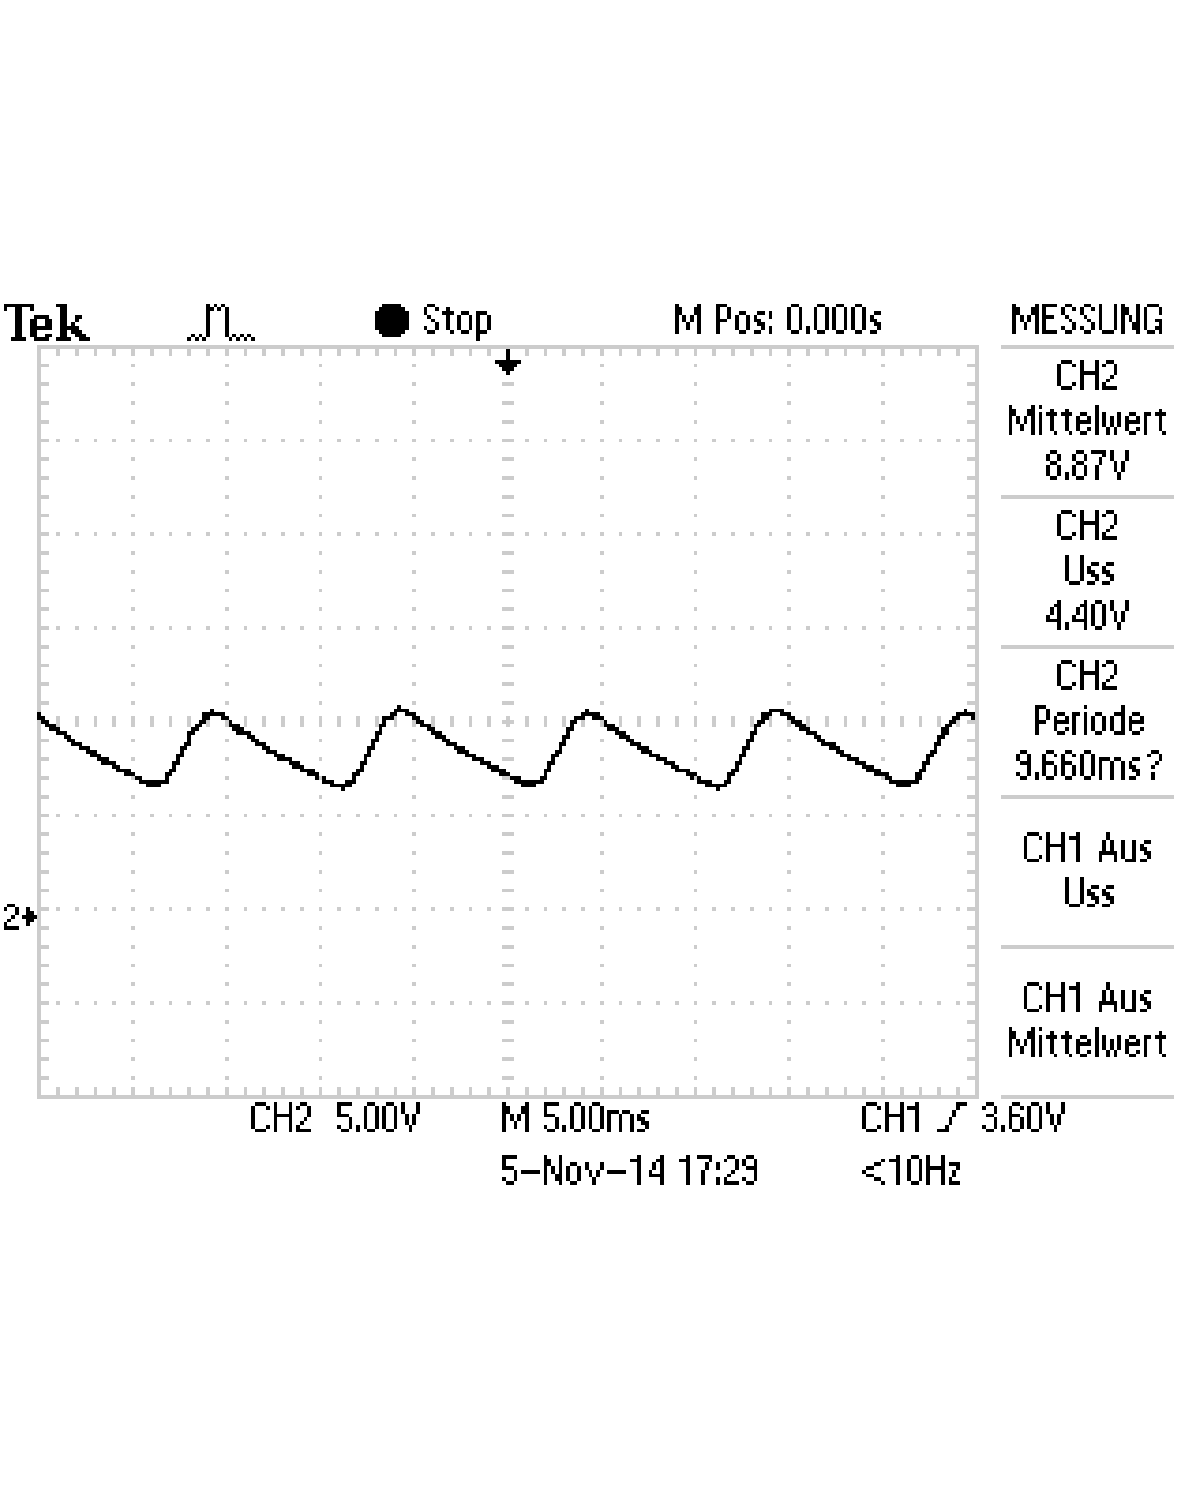
\includegraphics[width=\textwidth , scale = 0.4]{2_6_100F_2.pdf}
                \caption[Aufnahme bei minimalem Widerstand]{Aufnahme bei minimalem Widerstand}
  				\label{fig:2_6_100F_2}
        \end{subfigure}
        \caption{Aufnahme der Ausgangsspannung bei minimalem und maximalem Widerstand}
        \label{fig:2_6_100F}
\end{figure}

Für die 1000$\mu$F Kondensator ergaben sich die Verläufe aus Abbildung \ref{fig:2_6_1000F}.

\begin{figure}[H]
        \centering
        \begin{subfigure}[b]{0.48\textwidth}
                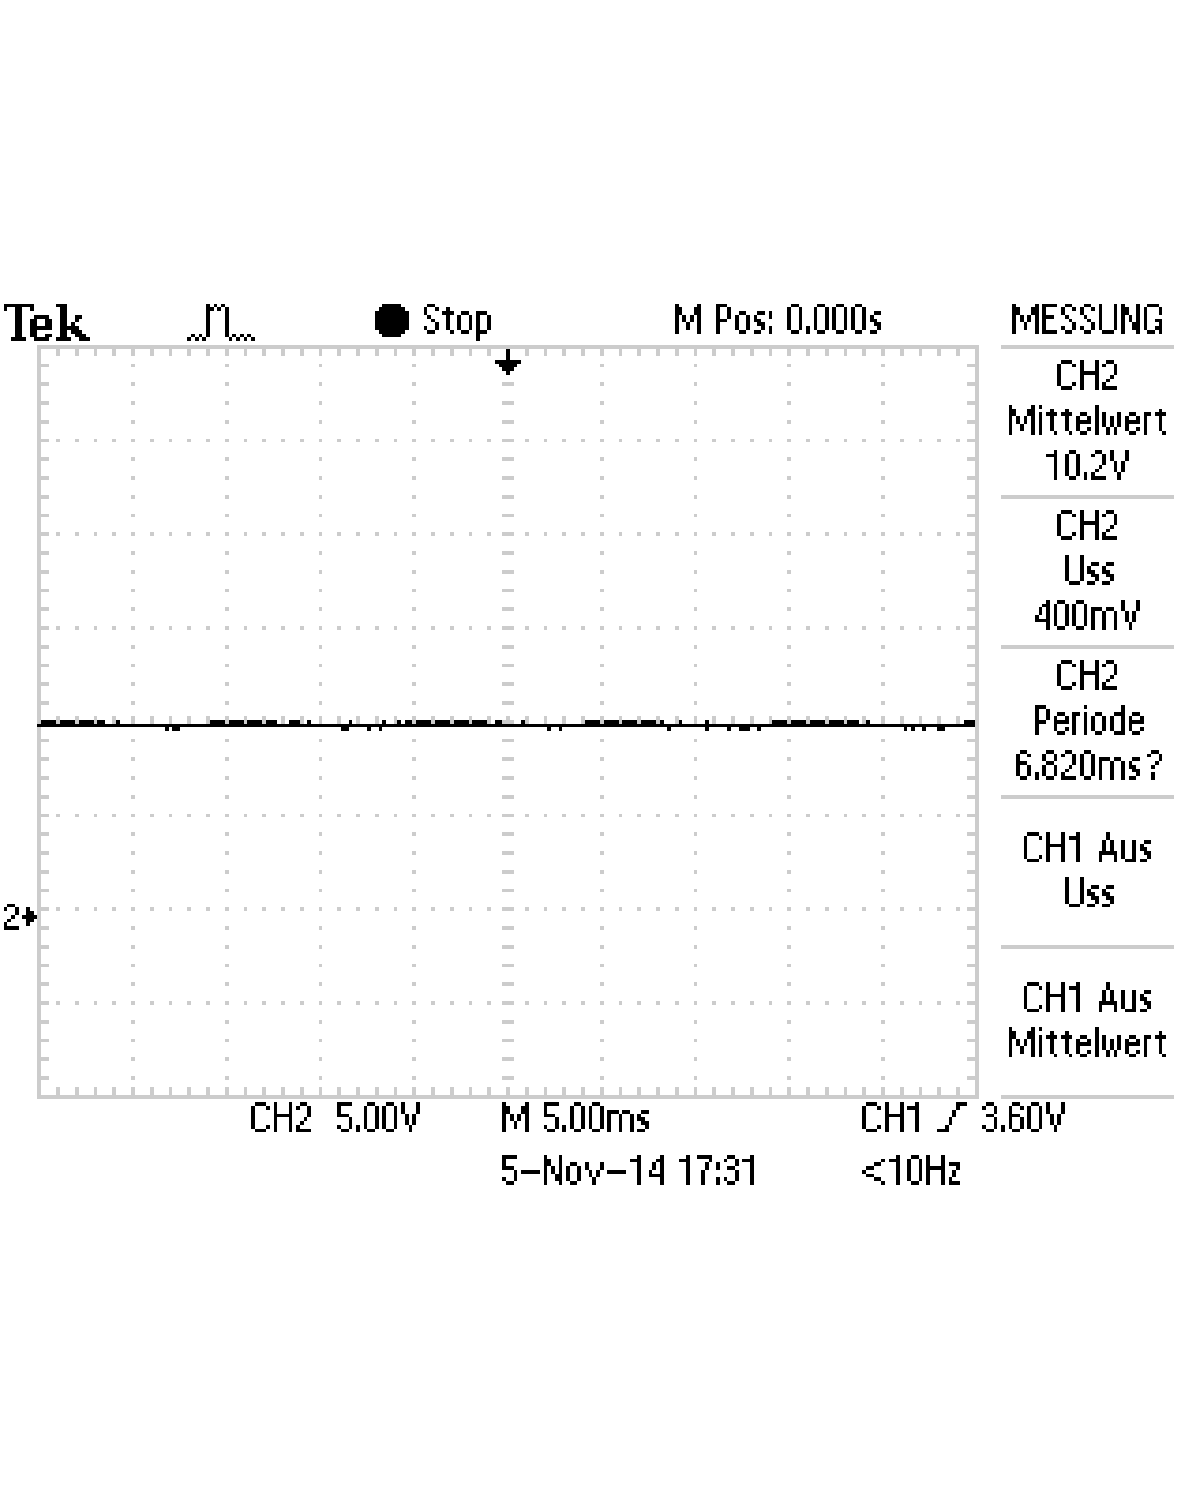
\includegraphics[width=\textwidth , scale = 0.4]{2_6_1000F_1.pdf}
                \caption[Aufnahme bei maximalem Widerstand]{Aufnahme bei maximalem Widerstand}
 				 \label{fig:2_6_1000F_1}
        \end{subfigure}%
        %~ %add desired spacing between images, e. g. ~, \quad, \qquad, \hfill etc.
          %(or a blank line to force the subfigure onto a new line)
        \hfill
        \begin{subfigure}[b]{0.48\textwidth}
                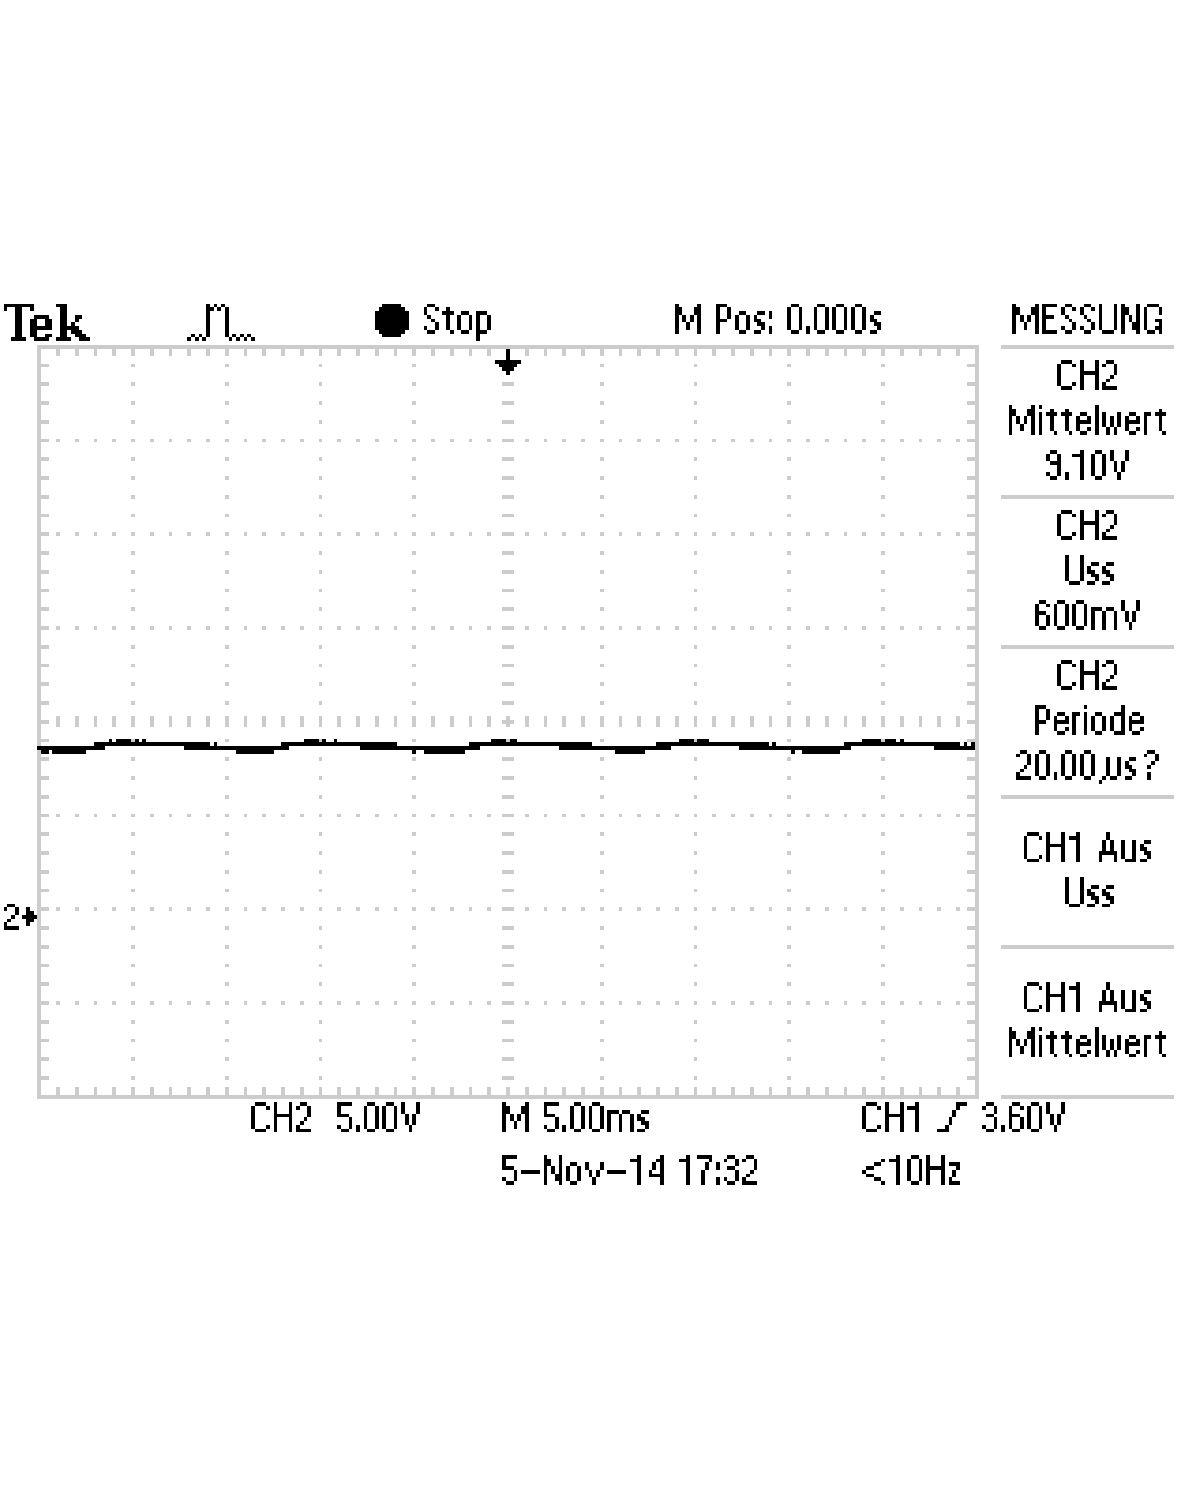
\includegraphics[width=\textwidth , scale = 0.4]{2_6_1000F_2.pdf}
                \caption[Aufnahme bei minimalem Widerstand]{Aufnahme bei minimalem Widerstand}
  				\label{fig:2_6_1000F_2}
        \end{subfigure}
        \caption{Aufnahme der Ausgangsspannung bei minimalem und maximalem Widerstand}
        \label{fig:2_6_1000F}
\end{figure}

Es ist deutlich zu erkennen, das der 1000$\mu$F Kondensator ein besseres Signal liefert.

\subsection{Diskussion}
%(immer) die gemessenen werte und die bestimmten werte über die messfehler mit literaturwerten oder untereinander vergleichen
%in welchem fehlerintervall des messwertes liegt der literaturwert oder der vergleichswert?
%wie ist der relative anteil des fehlers am messwert und damit die qualität unserer messung?
%in einem satz erklären, wie gut unser fehler und damit unsere messung ist
%kurz erläutern, wie systematische fehler unsere messung beeinflusst haben könnten
%(wichtig) zum schluss ansprechen, in wie weit die ergebnisse mit der theoretischen vorhersage übereinstimmen
%--------------------------------------------------------------------------------------------
%falls tabellen mit den messwerten zu lang werden, kann die section mit den messwerten auch hinter der diskussion angefügt bzw. eine section mit dem anhang eingefügt werden.

Wie erwartet wurde die halbe Zeit, in der kein Strom floss mit einem Kondensator überbrückt werden. Dabei zeigte sich, das bei Kondensatoren mit größerer Kapazität der Spitze-Spitze-Abstand geringer ausfiel, was auch erwartet wurde. 


\section{Spannungsstabilisierung}
%kurz das ziel dieses versuchsteiles ansprechen, damit keine zwei überschriften direkt übereinander stehen!
%bei schwierigeren versuchen kann auch der theoretische hintergrund erläutert werden. (mit formeln, herleitungen und erklärungen)
Ziel dieses Versuches ist die Spannung, welche an der Last abfällt, zu stabilisieren. Die Zenerdiode ist ein essentielles Bestandteil der verwendeten Schaltungen.

\subsection{Verwendete Materialien}
%(immer) eine skizze oder ein foto einfügen, die geräte/materialien !nummerieren! und z.b. eine legende dazu schreiben oder besser noch das ganze in einem Fließtext gut umschreiben
%falls am anfang des versuches nicht klar ist, was alles verwendet wird, wenn möglich erst am ende ein großes foto von den verwendeten materialien machen!

Zur Untersuchung der Ströme und Spannungen werden DMMs oder ein Oszilloskop verwendet. Als Stromquellen werden Funktionsgeneratoren oder Transformatoren verwendet. Als Bauteile werden Dioden, Widerstände, Potentiometer, Elektrolytkondenstoren, Glühlampen, ein Transistor und ein Spannungsregler Typ 7805 verwendet.

\subsection{Spannugsstabilisierung mit Zenerdiode (Transformatorbetrieb)}
Um die Spannung, welche an der Last abfällt, zu stabilisieren wird in den folgenden Versuchsteilen eine Zenerdiode verwendet.
\subsubsection{Versuchsaufbau}
%skizze zum versuchsaufbau (oder foto) einfügen,   es muss erklärt werden wie das ganze funktioniert und welche speziellen einstellungen verwendet wurden (z.b. welche knöpfe an den geräten für die messung verdreht wurden)
Der Kondensator hat eine Kapazität von 100$\mu$F oder 1000$\mu$F, Rv hat einen Widerstand von 200$\Omega$, für RL wird ein 470$\Omega$ Potentiometer verwendet und La ist eine Glühlampe.

\begin{figure}[H] 
  \centering
    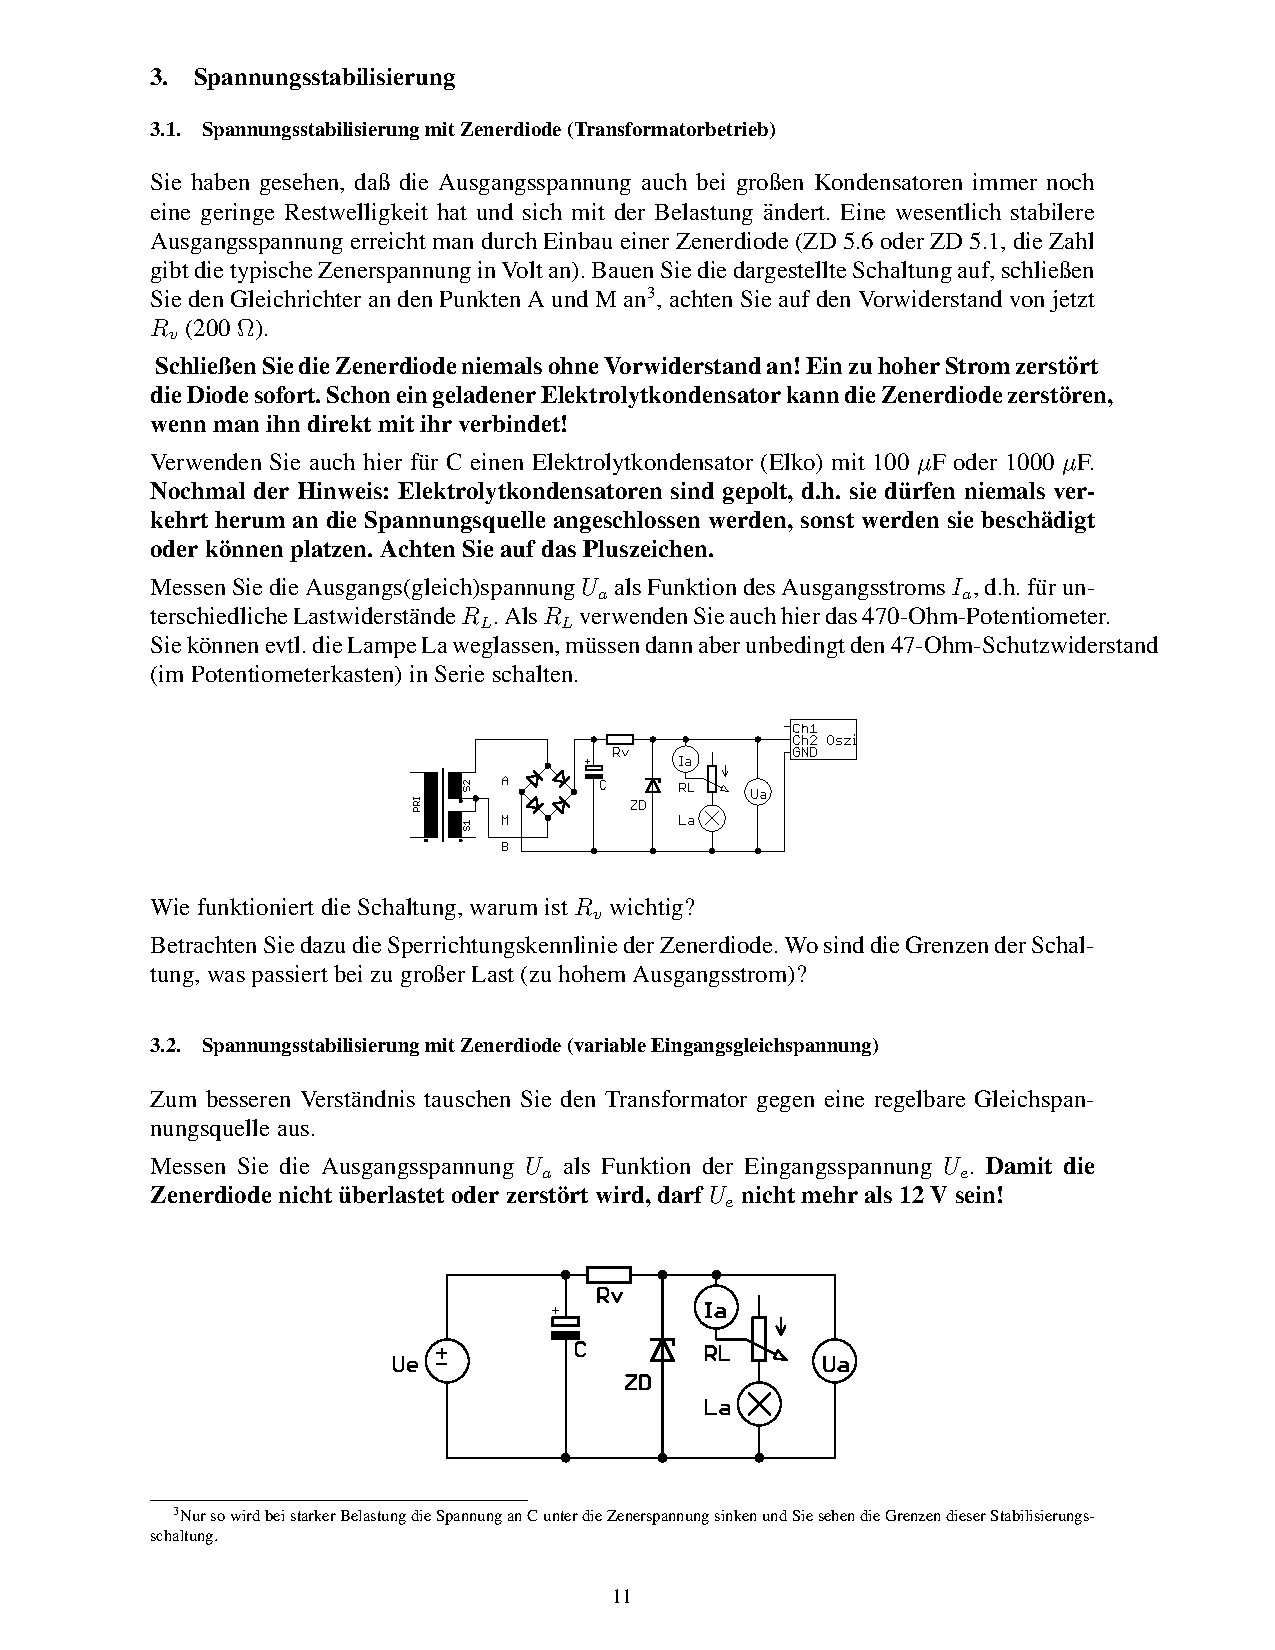
\includegraphics[trim = 10mm 130mm 10mm 120mm, clip, scale = 1]{ep2_14[Page11].pdf}
  	\caption[Schaltskizze zur Spannugsstabilisierung mit Zenerdiode]{Schaltskizze zur Spannugsstabilisierung mit Zenerdiode\footnotemark}
  \label{fig:2_8}
\end{figure}
\footnotetext{Abbildung entnommen von http://www.atlas.uni-wuppertal.de/$\sim$kind/ep2\_14.pdf Seite 10 am 28.10.2014}

\subsubsection{Versuchsdurchführung}
%erklären, !was! wir machen, !warum! wir das machen und mit welchem ziel
%(wichtig) präzize erklären, wie bei dem versuch vorgegangen und was gemacht wurde
Zur Spannungsstabilisierung wird eine Zenerdiode mit Vorwiderstand nach dem Schaltbild aus dem Versuchsaufbau \footnote{Versuchsaufbau: Abb. \ref{fig:2_8}} dazugeschaltet, sodass zu hohe Spannungen gefiltert werden. Der Vorwiderstand dient zum Schutz vor zu hohen Kondensatorspannungen. Bei minimalem und maximalem Potentiometerwiderstand und einer Kapazität von \unit[1000]{$\mu$F} wird der Strom und die Spannung durch bzw. über der Last gemessen, sowie die Ausgangsspannung am Oszilloskop aufgezeichnet. Nachteil bei dieser Schaltung ist die durch die Zenerdiode begrenzte Maximalspannung (\unit[5,1]{V}), wodurch auch die Leistung an der Last beschränkt wird.
\subsubsection{Messergebnisse}
%die messwerte in !übersichtlichen! tabellen angegeben
%zu viele kleine tabellen in große tabellen überführen!
%zu große tabellen mit dem [scale]-befehl scalieren oder (falls zu lang) in zwei kleinere tabellen aufteilen
%(wichtig) vor !jeder! tabelle sagen, was gemessen wurde und wie die fehler gewählt wurden und ausreichend !erklären!, !warum! wir unsere fehler grade so gewählt haben

Messdaten der Spannung und des Stroms.

\begin{table}[H]
\caption{Messdate der Ausgangsspannung in Abhängigkeit des Stroms}
\begin{center}
\begin{tabular}{|l|r|r|r|r|}
\hline
Widerstand & \multicolumn{1}{l|}{Spannung/V} & \multicolumn{1}{l|}{Fehler/V} & \multicolumn{1}{l|}{Strom/mA} & \multicolumn{1}{l|}{Fehler/A} \\ \hline
Max & 5,08 & 0,06 & 8,6 & 0,6 \\ \hline
Min & 3,54 & 0,06 & 31,3 & 0,6 \\ \hline
\end{tabular}
\end{center}
\label{tab:3_1}
\end{table}


\subsubsection{Auswertung}
%zuerst !alle! errechneten werte entweder in ganzen sätzen aufzählen, oder in tabellen (übersichtlicher) dargestellen, sowie auf die verwendeten formeln verweisen (die referenzierung der formel kann in der überschrift stehen)
%kurz erwähnen (vor der tabelle), warum wir das ganze ausrechnen bzw. was wir dort ausrechnen
%danach histogramme und plots erstellen, wobei wenn möglich funktionen durch die plots gelegt werden (zur not können auch splines benutzt werden, was aber angegeben werden muss)
%bei fits immer die funktion und das reduzierte chiquadrat mit angegeben, wobei auf verständlichkeit beim entziffern der zehnerpotenzen geachtet werden muss z.b. f(x)=(wert+-fehler)\cdot10^{irgendeine zahl}\cdot x + (wert+-fehler)\cdot10^{irgendeine zahl}
%bei jedem fit erklären, nach welchem zusammenhang gefittet wurde und warum!
%bei plots darauf achten, dass die achsenbeschriftung (auch die tics) die richtige größe haben und die legende im plot nicht die messwerte verdeckt
%kurz die aufgabenstellung abgehandeln

Es wurde die Ausgangsspannung in Abhängigkeit des Widerstandes des Potentiometers bestimmt werden. Es wurde eine Messung bei minimalem und bei maximalem Widerstand durchgeführt, die Messdaten sind in Abbildung \ref{fig:3_1} zu sehen. Jedoch wurde das Signal des Oszilloskops vor dem Vorwiderstand abgegriffen, dadurch liegt der Mittelwert bei 9,71V bzw. 9,74V und nicht bei 5,1V, was erwartet wurde. Jedoch war das DMM richtig angeschlossen und es wurden die erwarteten Werte gemessen, siehe Tabelle \ref{tab:3_1}.

\begin{figure}[H]
        \centering
        \begin{subfigure}[b]{0.48\textwidth}
                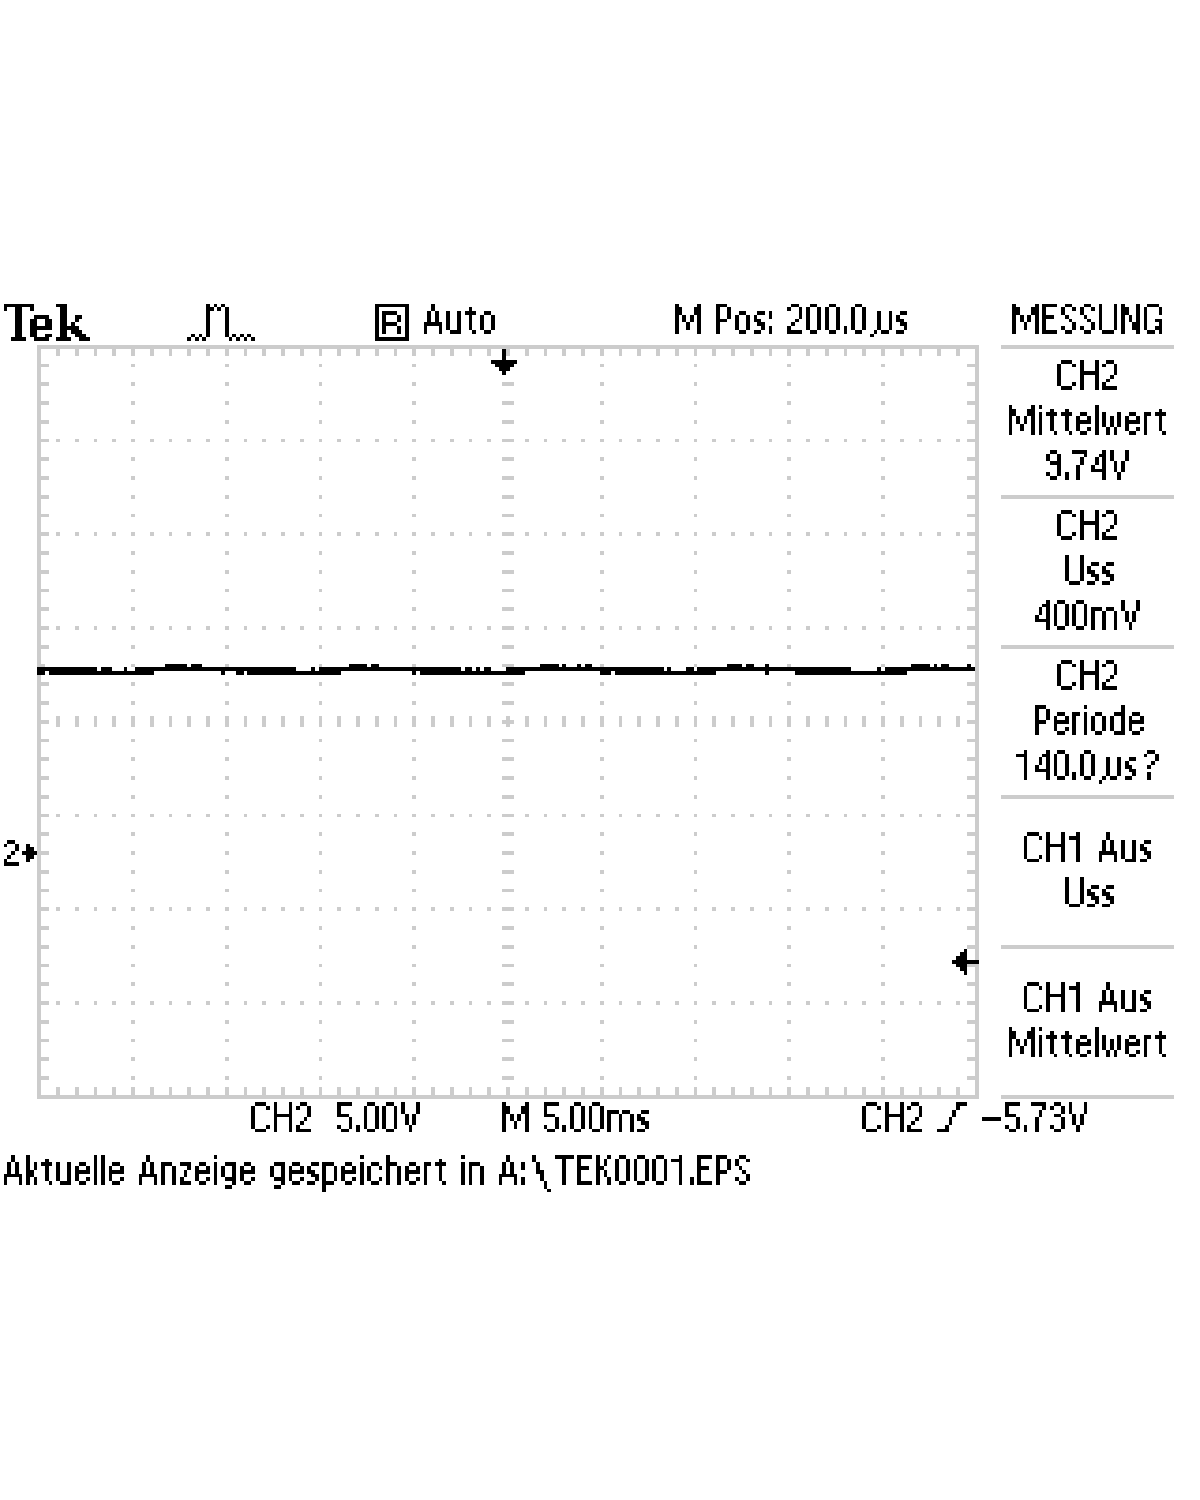
\includegraphics[width=\textwidth , scale = 0.4]{3_1_1.pdf}
                \caption[Aufnahme bei minimalem Widerstand]{Aufnahme bei minimalem Widerstand}
 				 \label{fig:3_1_1}
        \end{subfigure}%
        %~ %add desired spacing between images, e. g. ~, \quad, \qquad, \hfill etc.
          %(or a blank line to force the subfigure onto a new line)
        \hfill
        \begin{subfigure}[b]{0.48\textwidth}
                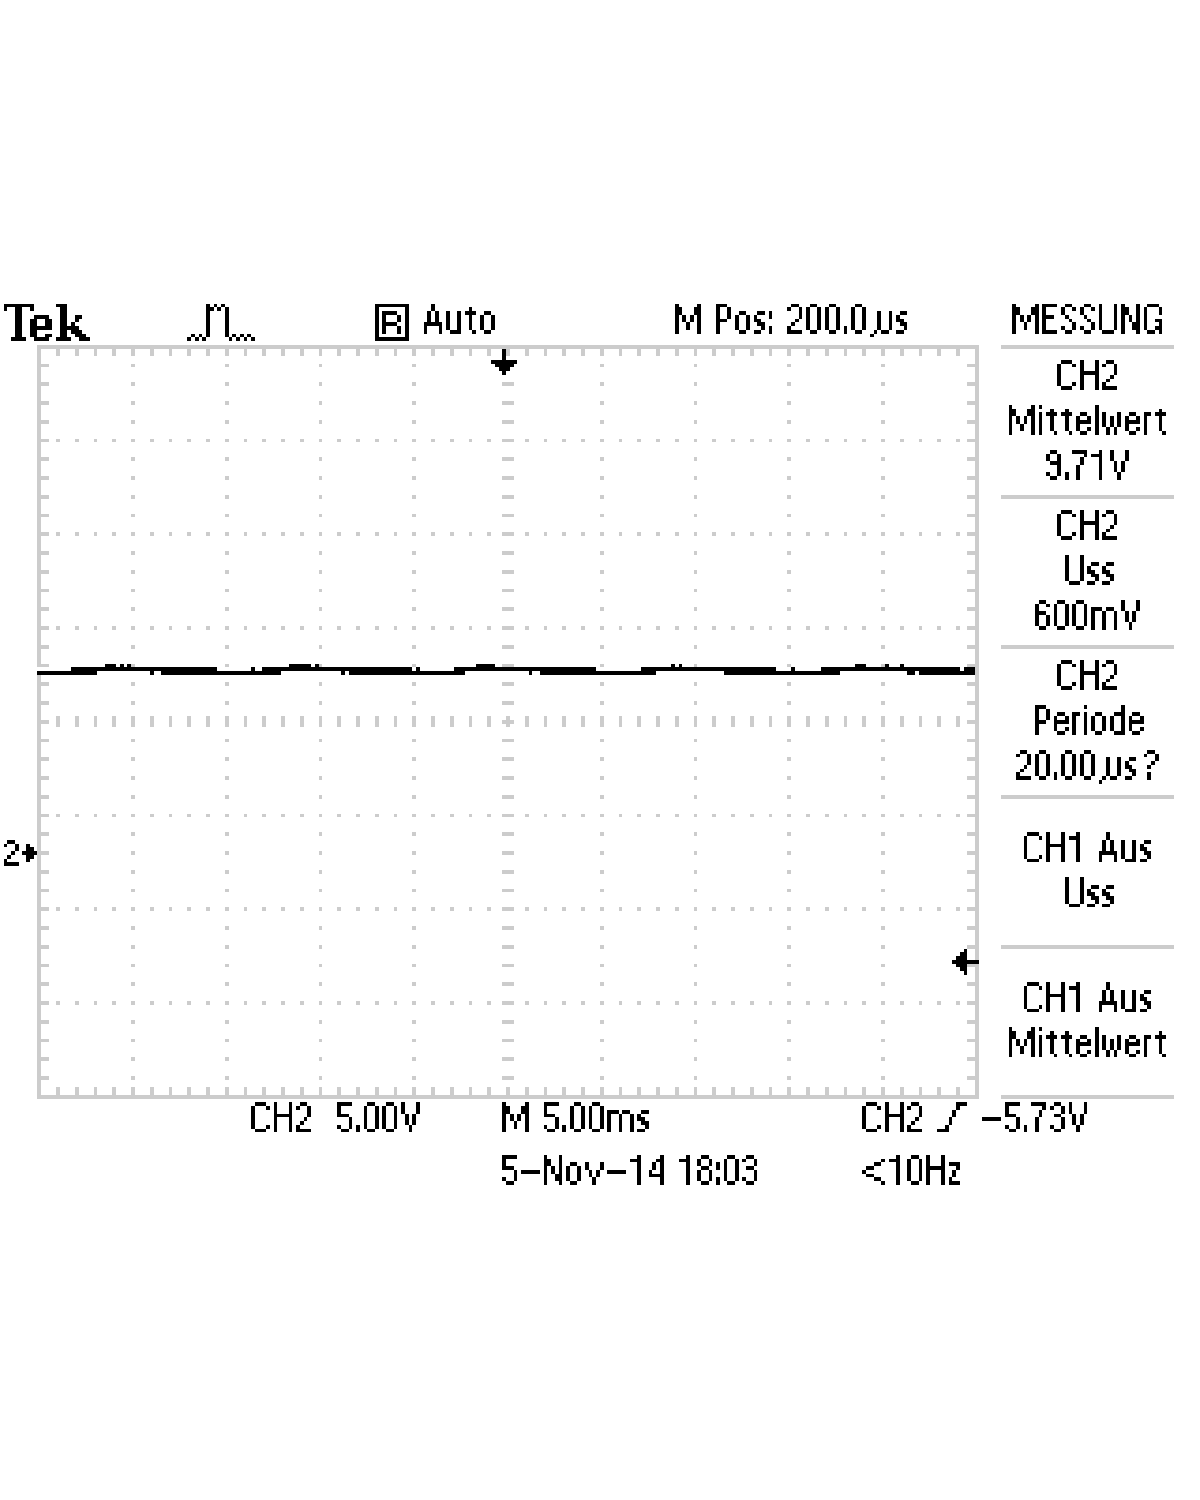
\includegraphics[width=\textwidth , scale = 0.4]{3_1_2.pdf}
                \caption[Aufnahme bei maximalem Widerstand]{Aufnahme bei maximalem Widerstand}
  				\label{fig:3_1_2}
        \end{subfigure}
        \caption{Aufnahme der Ausgangsspannung bei minimalem und maximalem Widerstand}
        \label{fig:3_1}
\end{figure}

Es ist zu sehen, dass bei geringerem Widerstand 400mV der Spitze-Spitze-Abstand geringer ist als bei dem maximalem Widerstand 600mV ist.
\subsection{Spannungstabilisierung mit Zenerdiode (variable Eingangsspannung)}
Der Trafo und die Brückengleichrichterschaltung wird nun durch eine variable Gleichspannungsquelle ersetzt, um die Ausgangsspannung abhängig von der Eingangsspannung darzustellen.
\subsubsection{Versuchsaufbau}
%skizze zum versuchsaufbau (oder foto) einfügen,   es muss erklärt werden wie das ganze funktioniert und welche speziellen einstellungen verwendet wurden (z.b. welche knöpfe an den geräten für die messung verdreht wurden)

Die Bauteile haben die selben Werte wie im vorherigem Aufbau jedoch wurde die Brückengleichrichterschaltung entfernt.

\begin{figure}[H] 
  \centering
    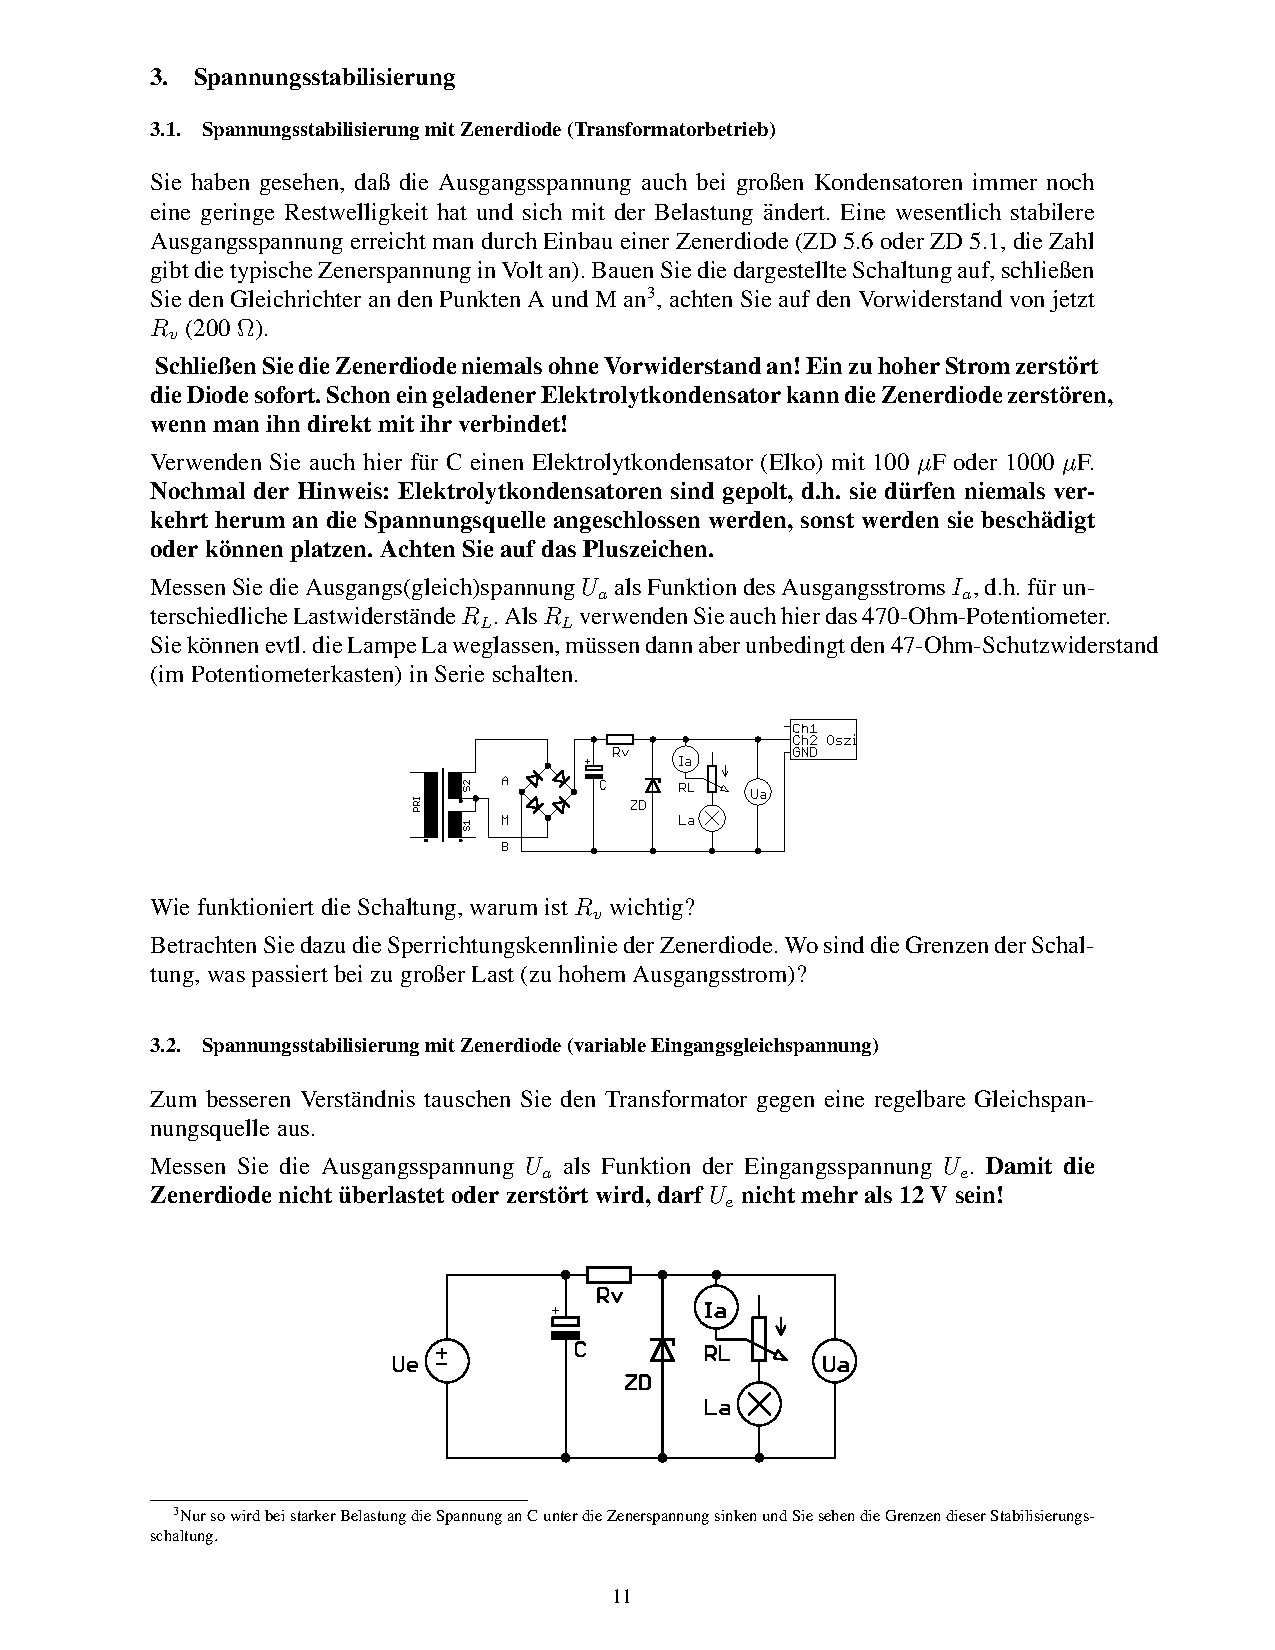
\includegraphics[trim = 10mm 30mm 10mm 213mm, clip, scale = 1]{ep2_14[Page11].pdf}
  	\caption[Schaltskizze zur Spannugsstabilisierung mit Zenerdiode, bei variabler Eingangsspannung]{Schaltskizze zur Spannugsstabilisierung mit Zenerdiode, bei variabler Eingangsspannung\footnotemark}
  \label{fig:2_9}
\end{figure}
\footnotetext{Abbildung entnommen von http://www.atlas.uni-wuppertal.de/$\sim$kind/ep2\_14.pdf Seite 10 am 28.10.2014}


\subsubsection{Versuchsdurchführung}
%erklären, !was! wir machen, !warum! wir das machen und mit welchem ziel
%(wichtig) präzize erklären, wie bei dem versuch vorgegangen und was gemacht wurde
Der Trafo und die Brückengleichrichterschaltung werden durch eine variable Eingangsgleichspannung (Funktionsgenerator) ersetzt \footnote{Versuchsaufbau: Abb. \ref{fig:2_9}}. Bei variierender Eingangsspannung wird Strom und Spannung über der Last gemessen (DMM) und geplottet \footnote{Da bei diesem Versuchsteil Gleichspannung herrscht, ist der Kondensator relativ unwichtig. Im folgenden Versuchsteil wird er deshalb einfach weggelassen.}.
\subsubsection{Messergebnisse}
%die messwerte in !übersichtlichen! tabellen angegeben
%zu viele kleine tabellen in große tabellen überführen!
%zu große tabellen mit dem [scale]-befehl scalieren oder (falls zu lang) in zwei kleinere tabellen aufteilen
%(wichtig) vor !jeder! tabelle sagen, was gemessen wurde und wie die fehler gewählt wurden und ausreichend !erklären!, !warum! wir unsere fehler grade so gewählt haben

Der Fehler für den Strom und U$_\text{aus}$ wurden mit dem angegebenen Fehler und der Ableseungenauigkeit bestimmt, sie liegen bei 0,06V und 0,06mA. Der Fehler der Eingangsspannung wurde nur über die Ableseungenauigkeit bestimmt, das kein Fehlerwert angegeben war.

\begin{table}[H]
\caption{Messung der Ausgangsspannung und des Stroms in Abhängigkeit der Eingangsspannung}
\begin{center}
\begin{tabular}{|r|r|r|}
\hline
\multicolumn{1}{|l|}{U$_\text{ein}$/V} & \multicolumn{1}{l|}{U$_\text{aus}$/V} & \multicolumn{1}{l|}{Strom/mA} \\ \hline
1 & 1,01 & 0,98 \\ \hline
2 & 2,1 & 1,98 \\ \hline
3 & 3,06 & 2,97 \\ \hline
4 & 4,02 & 3,93 \\ \hline
5 & 4,72 & 4,87 \\ \hline
6 & 4,96 & 5,83 \\ \hline
7 & 5,03 & 6,74 \\ \hline
8 & 5,08 & 7,52 \\ \hline
9 & 5,1 & 8,08 \\ \hline
10 & 5,12 & 8,31 \\ \hline
11 & 5,14 & 8,48 \\ \hline
12 & 5,16 & 8,57 \\ \hline
\end{tabular}
\end{center}
\label{tab:3_2_w}
\end{table}


\subsubsection{Auswertung}
%zuerst !alle! errechneten werte entweder in ganzen sätzen aufzählen, oder in tabellen (übersichtlicher) dargestellen, sowie auf die verwendeten formeln verweisen (die referenzierung der formel kann in der überschrift stehen)
%kurz erwähnen (vor der tabelle), warum wir das ganze ausrechnen bzw. was wir dort ausrechnen
%danach histogramme und plots erstellen, wobei wenn möglich funktionen durch die plots gelegt werden (zur not können auch splines benutzt werden, was aber angegeben werden muss)
%bei fits immer die funktion und das reduzierte chiquadrat mit angegeben, wobei auf verständlichkeit beim entziffern der zehnerpotenzen geachtet werden muss z.b. f(x)=(wert+-fehler)\cdot10^{irgendeine zahl}\cdot x + (wert+-fehler)\cdot10^{irgendeine zahl}
%bei jedem fit erklären, nach welchem zusammenhang gefittet wurde und warum!
%bei plots darauf achten, dass die achsenbeschriftung (auch die tics) die richtige größe haben und die legende im plot nicht die messwerte verdeckt
%kurz die aufgabenstellung abgehandeln

Wie in Abbildung \ref{fig:3_2} zu sehen ist, wird die Ausgangsspannung bei einem Wert von 5,1V von der Zenerdiode abgeschnitten.

\begin{figure}[H] 
  \centering
    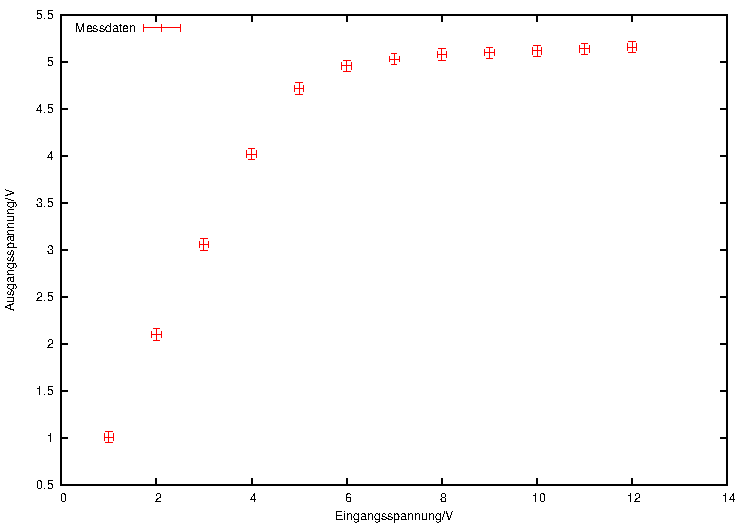
\includegraphics[ scale = 0.7]{3_2.pdf}
  	\caption[Ausgangsspannung in Abhängigkeit der Eingangsspannung]{Ausgangsspannung in Abhängigkeit der Eingangsspannung}
  \label{fig:3_2}
\end{figure}

\subsection{Erhöhung des Ausgangsstroms mit Transistor}
Ein Transistor, welcher den Ausgangsstrom erhöhen soll wird nun dazu geschaltet. Der Vorteil dieser Schaltung besteht darin, dass eine höhere Leistung an der Last erzielt werden kann. 
\subsubsection{Versuchsaufbau}
%skizze zum versuchsaufbau (oder foto) einfügen,   es muss erklärt werden wie das ganze funktioniert und welche speziellen einstellungen verwendet wurden (z.b. welche knöpfe an den geräten für die messung verdreht wurden)

T1 ist ein Transistor, R1 ein 470 $\Omega$ Widerstand, R2 ein 470$\Omega$ Potentiometer, R3 der eingebaute Vorwiderstand des Potentiometers.

\begin{figure}[H] 
  \centering
    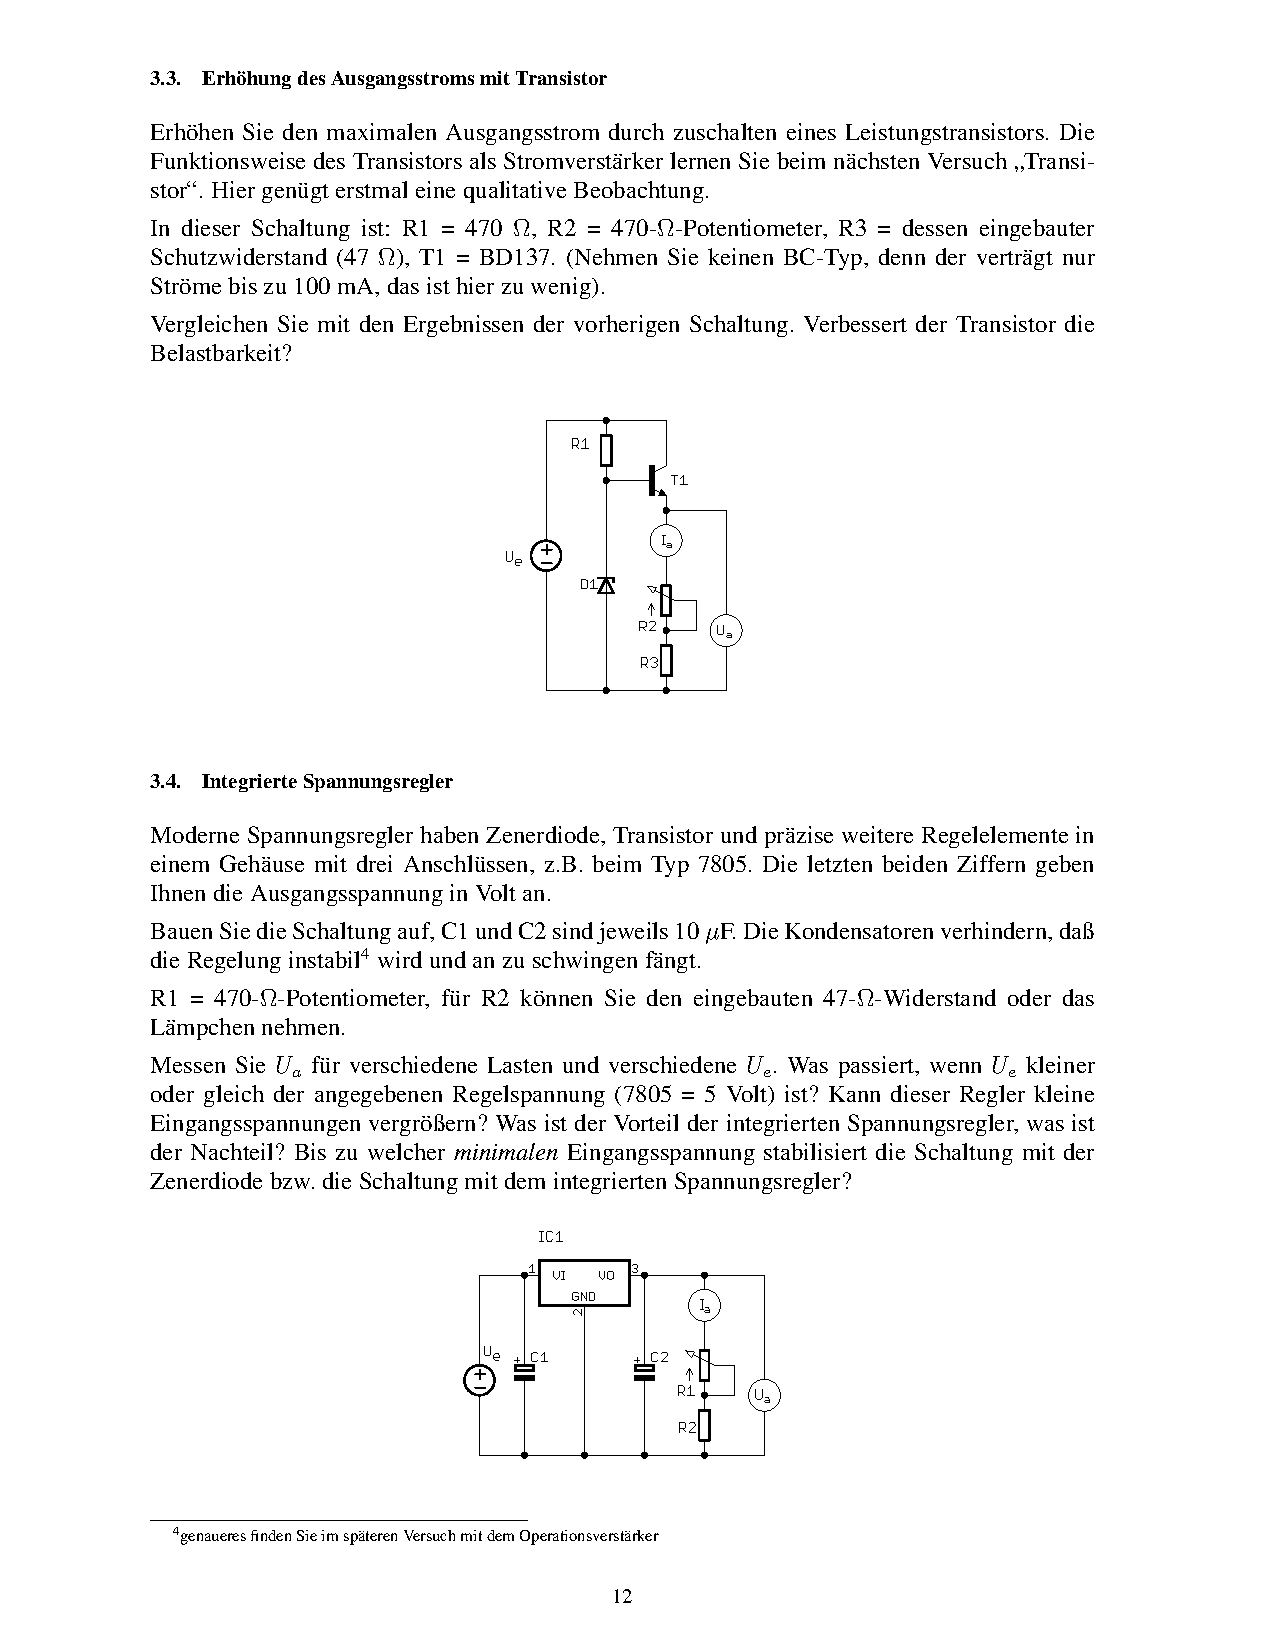
\includegraphics[trim = 10mm 160mm 10mm 70mm, clip, scale = 1]{ep2_14[Page12].pdf}
  	\caption[Schaltskizze zur Spannugsstabilisierung mit Zenerdiode, bei variabler Eingangsspannung]{Schaltskizze zur Spannugsstabilisierung mit Zenerdiode, bei variabler Eingangsspannung\footnotemark}
  \label{fig:2_10}
\end{figure}
\footnotetext{Abbildung entnommen von http://www.atlas.uni-wuppertal.de/$\sim$kind/ep2\_14.pdf Seite 10 am 28.10.2014}

\subsubsection{Versuchsdurchführung}
%erklären, !was! wir machen, !warum! wir das machen und mit welchem ziel
%(wichtig) präzize erklären, wie bei dem versuch vorgegangen und was gemacht wurde
In diesem Versuchsteil soll der Ausgangsstrom mithilfe eines Transitors erhöht werden\footnote{Versuchsaufbau: Abb. \ref{fig:2_10}}. Damit kann an der Last eine höhere Leistung erzielt werden. Strom und Spannung werden mithilfe zweier DMM aufgenommen und geplottet.
\subsubsection{Messergebnisse}
%die messwerte in !übersichtlichen! tabellen angegeben
%zu viele kleine tabellen in große tabellen überführen!
%zu große tabellen mit dem [scale]-befehl scalieren oder (falls zu lang) in zwei kleinere tabellen aufteilen
%(wichtig) vor !jeder! tabelle sagen, was gemessen wurde und wie die fehler gewählt wurden und ausreichend !erklären!, !warum! wir unsere fehler grade so gewählt haben

Der Fehler für den Strom und U$_\text{aus}$ wurden mit dem angegebenen Fehler und der Ableseungenauigkeit bestimmt, sie liegen bei 0,06V und 0,006A. Der Fehler der Eingangsspannung wurde nur über die Ableseungenauigkeit bestimmt, das kein Fehlerwert angegeben war.

\begin{table}[H]
\caption{Messung der Ausgangsspannung und des Stroms in Abhängigkeit der Eingangsspannung}
\begin{center}
\begin{tabular}{|r|r|r|}
\hline
\multicolumn{1}{|l|}{U$_\text{ein}$/V} & \multicolumn{1}{l|}{U$_\text{aus}$/V} & \multicolumn{1}{l|}{Strom/A} \\ \hline
1 & 0,34 & 0,07 \\ \hline
2 & 1,15 & 0,024 \\ \hline
3 & 2,02 & 0,042 \\ \hline
4 & 2,89 & 0,06 \\ \hline
5 & 3,56 & 0,075 \\ \hline
6 & 3,97 & 0,083 \\ \hline
7 & 4,15 & 0,87 \\ \hline
8 & 4,23 & 0,089 \\ \hline
9 & 4,28 & 0,09 \\ \hline
10 & 4,32 & 0,91 \\ \hline
11 & 4,35 & 0,91 \\ \hline
12 & 4,37 & 0,092 \\ \hline
\end{tabular}
\end{center}
\label{tab:3_3_w}
\end{table}


\subsubsection{Auswertung}
%zuerst !alle! errechneten werte entweder in ganzen sätzen aufzählen, oder in tabellen (übersichtlicher) dargestellen, sowie auf die verwendeten formeln verweisen (die referenzierung der formel kann in der überschrift stehen)
%kurz erwähnen (vor der tabelle), warum wir das ganze ausrechnen bzw. was wir dort ausrechnen
%danach histogramme und plots erstellen, wobei wenn möglich funktionen durch die plots gelegt werden (zur not können auch splines benutzt werden, was aber angegeben werden muss)
%bei fits immer die funktion und das reduzierte chiquadrat mit angegeben, wobei auf verständlichkeit beim entziffern der zehnerpotenzen geachtet werden muss z.b. f(x)=(wert+-fehler)\cdot10^{irgendeine zahl}\cdot x + (wert+-fehler)\cdot10^{irgendeine zahl}
%bei jedem fit erklären, nach welchem zusammenhang gefittet wurde und warum!
%bei plots darauf achten, dass die achsenbeschriftung (auch die tics) die richtige größe haben und die legende im plot nicht die messwerte verdeckt
%kurz die aufgabenstellung abgehandeln

Wie in Abbildung \ref{fig:3_2} zu sehen ist, wird die Ausgangsspannung bei einem Wert von 4,3V, wie im vorherigem Versuchsteil von der Zenerdiode abgeschnitten.

\begin{figure}[H] 
  \centering
    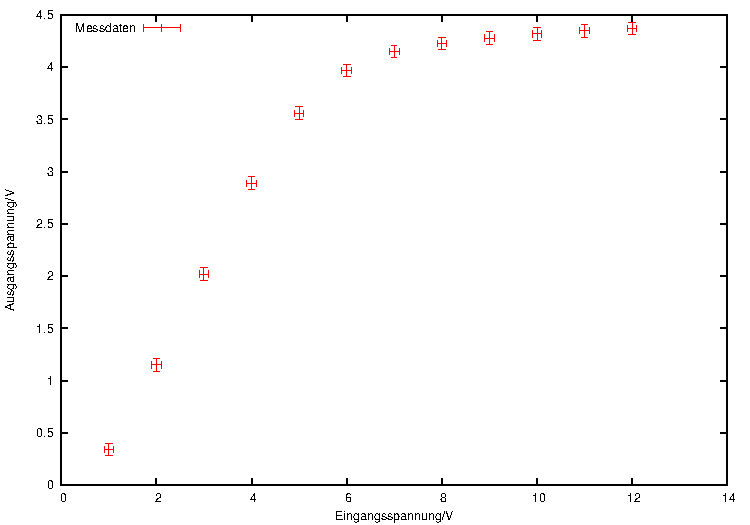
\includegraphics[ scale = 0.7]{3_3.pdf}
  	\caption[Ausgangsspannung in Abhängigkeit der Eingangsspannung]{Ausgangsspannung in Abhängigkeit der Eingangsspannung}
  \label{fig:3_3}
\end{figure}

Jedoch ist die Leistung höher als im Vorherigem Aufbau. Dies lässt sich aus den Werten für den Strom in Tabelle \ref{tab:3_2_w} und Tabelle \ref{tab:3_3_w} ablesen.

\subsection{Integrierte Spannungsregler}
Es wird ein Integrierter Spannungsregler (Typ 7805) verwendet.
\subsubsection{Versuchsaufbau}
%skizze zum versuchsaufbau (oder foto) einfügen,   es muss erklärt werden wie das ganze funktioniert und welche speziellen einstellungen verwendet wurden (z.b. welche knöpfe an den geräten für die messung verdreht wurden)

C1 und C2 sind 10$\mu$F, R1 ist ein 470 Potentiometer und R2 dessen eingebauter Vorwiderstand, IC1 ist ein Regelelement des Typs 7805.

\begin{figure}[H] 
  \centering
    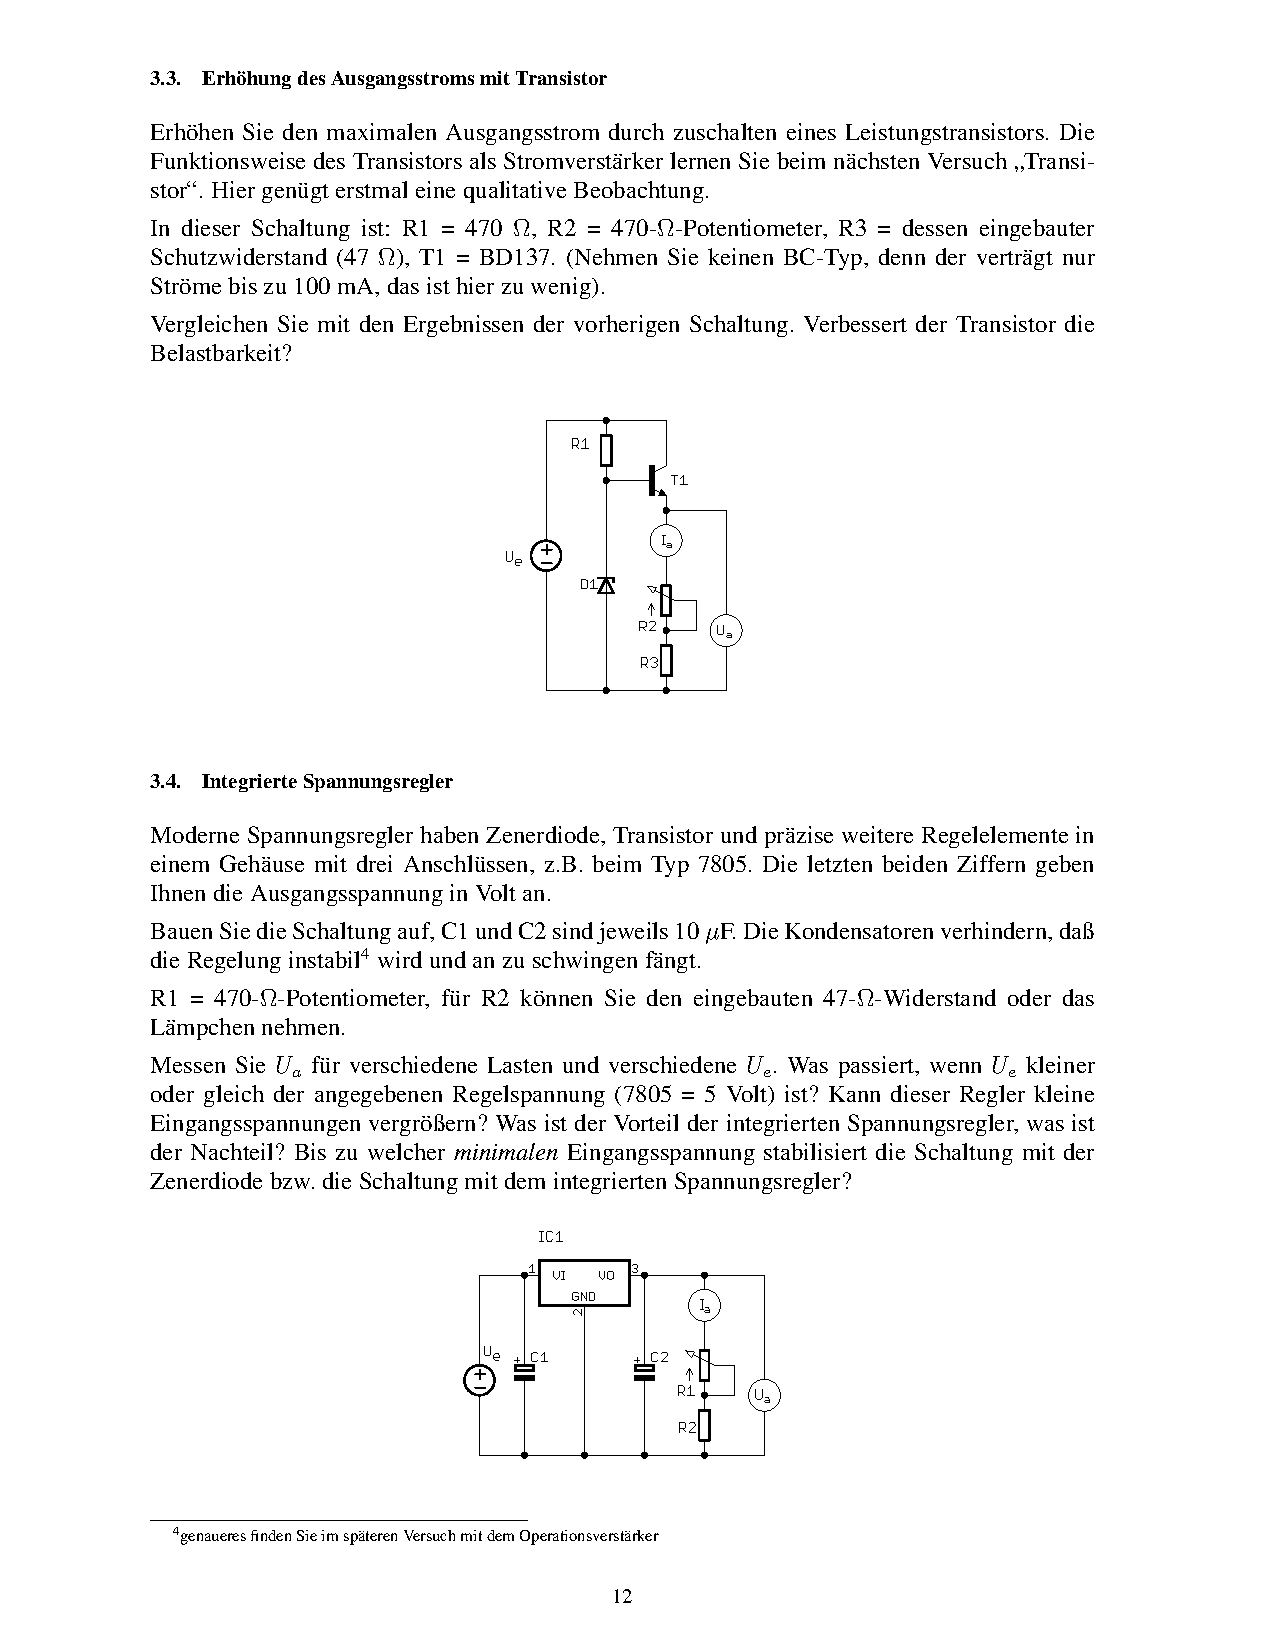
\includegraphics[trim = 10mm 30mm 10mm 205mm, clip, scale = 1]{ep2_14[Page12].pdf}
  	\caption[Schaltskizze zur Spannugsstabilisierung mit Zenerdiode, bei variabler Eingangsspannung]{Schaltskizze zur Spannugsstabilisierung mit Zenerdiode, bei variabler Eingangsspannung\footnotemark}
  \label{fig:2_11}
\end{figure}
\footnotetext{Abbildung entnommen von http://www.atlas.uni-wuppertal.de/$\sim$kind/ep2\_14.pdf Seite 10 am 28.10.2014}

\subsubsection{Versuchsdurchführung}
%erklären, !was! wir machen, !warum! wir das machen und mit welchem ziel
%(wichtig) präzize erklären, wie bei dem versuch vorgegangen und was gemacht wurde
Im letzten Versuchsteil soll ein moderner Spannungsregler untersucht und mit den anderen Schaltungen verglichen werden\footnote{Versuchsaufbau: Abb. \ref{fig:2_11}}. Strom und Spannung werden mithilfe zweier DMM aufgenommen und geplottet.
\subsubsection{Messergebnisse}
%die messwerte in !übersichtlichen! tabellen angegeben
%zu viele kleine tabellen in große tabellen überführen!
%zu große tabellen mit dem [scale]-befehl scalieren oder (falls zu lang) in zwei kleinere tabellen aufteilen
%(wichtig) vor !jeder! tabelle sagen, was gemessen wurde und wie die fehler gewählt wurden und ausreichend !erklären!, !warum! wir unsere fehler grade so gewählt haben

Der Fehler für den Strom und die Ausgagnsspannung wurden über die Ableseungenauigkeit und den Angegebenen Fehler bestimmt, dabei ergibt sich ein Wert von 0,06V und 0,06mA. Der Fehler der Eingagansspannung wurde nur über die Ableseungenauigkeit bestimmt, es ergibt sich ein Wert von 0,1V.

\begin{table}[H]
\caption{Messung der Aus- und Eingagnsspannung, sowie des Stromes, bei minimalem Widerstand}
\begin{center}
\begin{tabular}{|r|r|r|}
\hline
\multicolumn{1}{|l|}{U$_\text{ein}$/V} & \multicolumn{1}{l|}{U$_\text{aus}$/V} & \multicolumn{1}{l|}{Strom/mA} \\ \hline
1 & 0 & 0 \\ \hline
2 & 0 & 0,01 \\ \hline
3 & 1,81 & 3,28 \\ \hline
4 & 2,81 & 5,08 \\ \hline
5 & 3,77 & 6,82 \\ \hline
6 & 4,72 & 8,53 \\ \hline
7 & 4,94 & 8,94 \\ \hline
8 & 4,94 & 8,94 \\ \hline
9 & 4,94 & 8,94 \\ \hline
10 & 4,94 & 8,94 \\ \hline
\end{tabular}
\end{center}
\label{tab:3_4_min}
\end{table}

Die Fehler wurden wie oben angenommen, da die selben Messapparaturen verwendet wurden.

\begin{table}[H]
\caption{Messung der Aus- und Eingagnsspannung, sowie des Stromes, bei maximalem Widerstand}
\begin{center}
\begin{tabular}{|r|r|r|}
\hline
\multicolumn{1}{|l|}{U$_\text{ein}$/V} & \multicolumn{1}{l|}{U$_\text{aus}$/V} & \multicolumn{1}{l|}{Strom/mA} \\ \hline
1 & 0 & 0 \\ \hline
2 & 0 & 0 \\ \hline
3 & 1,72 & 35,7 \\ \hline
4 & 2,68 & 55,6 \\ \hline
5 & 3,66 & 76,1 \\ \hline
6 & 4,6 & 95,8 \\ \hline
7 & 4,93 & 102,6 \\ \hline
8 & 4,93 & 102,6 \\ \hline
9 & 4,93 & 102,6 \\ \hline
10 & 4,93 & 102,6 \\ \hline
\end{tabular}
\end{center}
\label{tab:3_4_max}
\end{table}


\subsubsection{Auswertung}
%zuerst !alle! errechneten werte entweder in ganzen sätzen aufzählen, oder in tabellen (übersichtlicher) dargestellen, sowie auf die verwendeten formeln verweisen (die referenzierung der formel kann in der überschrift stehen)
%kurz erwähnen (vor der tabelle), warum wir das ganze ausrechnen bzw. was wir dort ausrechnen
%danach histogramme und plots erstellen, wobei wenn möglich funktionen durch die plots gelegt werden (zur not können auch splines benutzt werden, was aber angegeben werden muss)
%bei fits immer die funktion und das reduzierte chiquadrat mit angegeben, wobei auf verständlichkeit beim entziffern der zehnerpotenzen geachtet werden muss z.b. f(x)=(wert+-fehler)\cdot10^{irgendeine zahl}\cdot x + (wert+-fehler)\cdot10^{irgendeine zahl}
%bei jedem fit erklären, nach welchem zusammenhang gefittet wurde und warum!
%bei plots darauf achten, dass die achsenbeschriftung (auch die tics) die richtige größe haben und die legende im plot nicht die messwerte verdeckt
%kurz die aufgabenstellung abgehandeln

Wie in Abbildung \ref{fig:3_4_min_v} und \ref{fig:3_4_max_v} zu erkennen ist hängt die Ausgangsspannung von der Eingangsspannung ab. Danach ist die Ausgangsspannung unabhängig von der Eingangsspannung. Die stabilisierung der Spannung fängt ab 6V an.

\begin{figure}[H] 
  \centering
    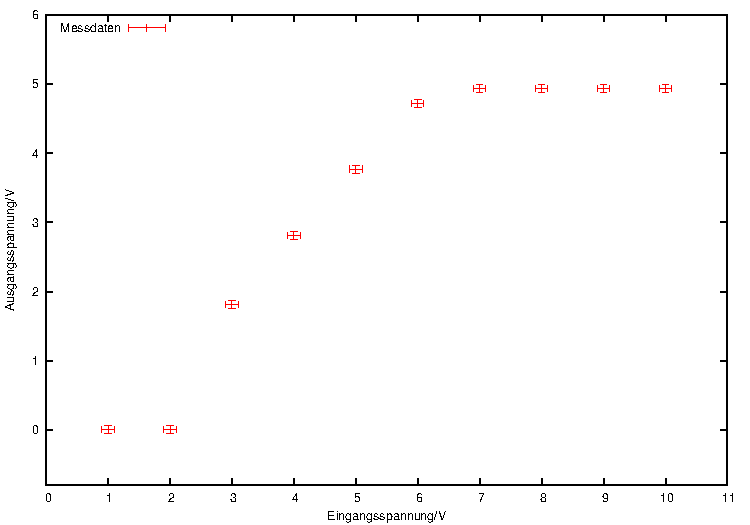
\includegraphics[ scale = 0.7]{3_4_min_v.pdf}
  	\caption[Ausgangsspannung in Abhängigkeit der Eingangsspannung, bei minimalem Widerstand]{Ausgangsspannung in Abhängigkeit der Eingangsspannung, bei minimalem Widerstand}
  \label{fig:3_4_min_v}
\end{figure}


\begin{figure}[H] 
  \centering
    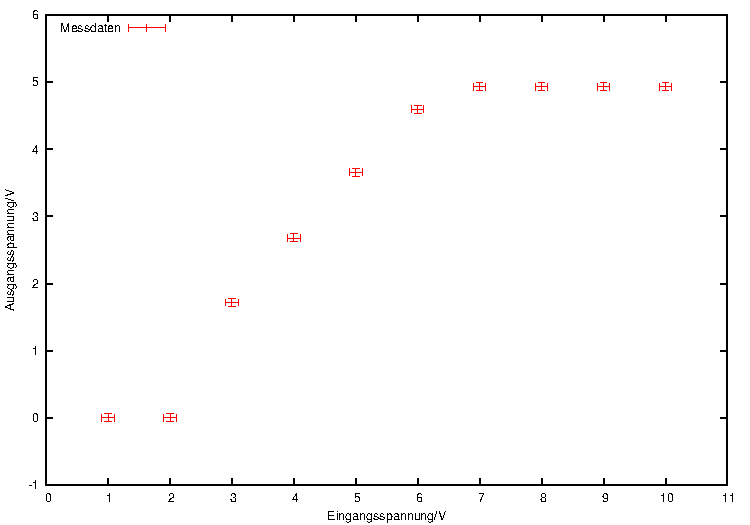
\includegraphics[ scale = 0.7]{3_4_max_v.pdf}
  	\caption[Ausgangsspannung in Abhängigkeit der Eingangsspannung, bei maximalem Widerstand]{Ausgangsspannung in Abhängigkeit der Eingangsspannung, bei maximalem Widerstand}
  \label{fig:3_4_max_v}
\end{figure}

Plottet man den Strom gegen die Eingangsspannung erbeben sich die Verläufe in Abbildung \ref{fig:3_4_min_a} und Abbildung \ref{fig:3_4_max_a} für den minimalen und den maximalen Widerstand.

\begin{figure}[H] 
  \centering
    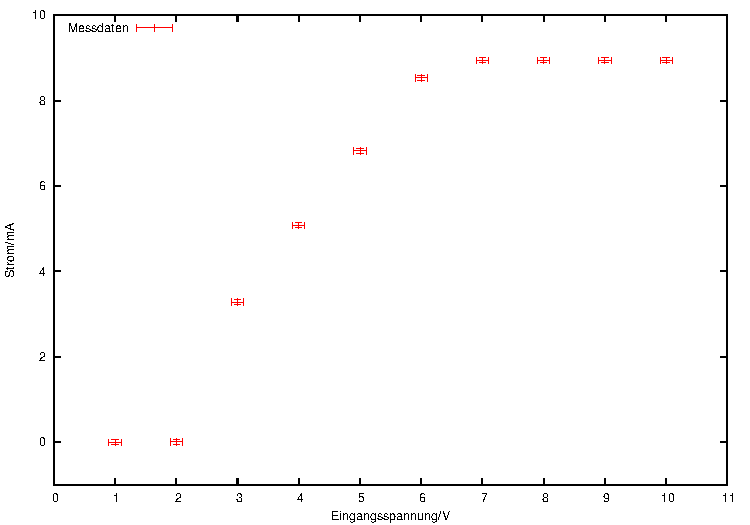
\includegraphics[ scale = 0.7]{3_4_min_a.pdf}
  	\caption[Ausgangsspannung in Abhängigkeit der Eingangsspannung, bei minimalem Widerstand]{Ausgangsspannung in Abhängigkeit der Eingangsspannung, bei minimalem Widerstand}
  \label{fig:3_4_min_a}
\end{figure}


\begin{figure}[H] 
  \centering
    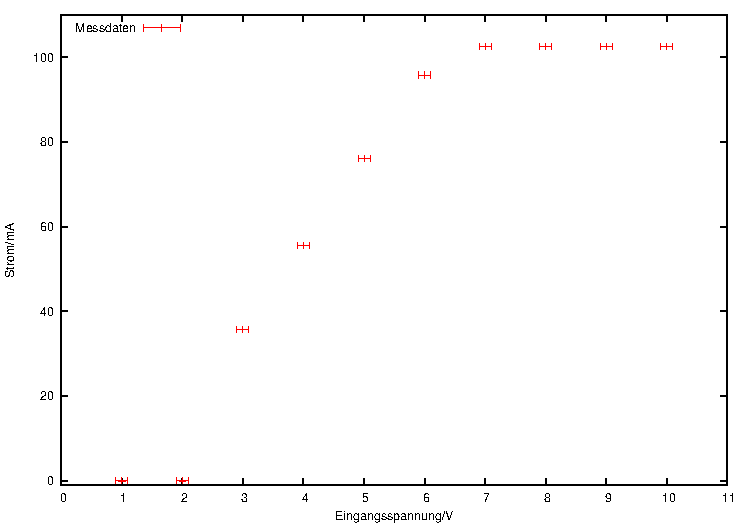
\includegraphics[ scale = 0.7]{3_4_max_a.pdf}
  	\caption[Ausgangsspannung in Abhängigkeit der Eingangsspannung, bei maximalem Widerstand]{Ausgangsspannung in Abhängigkeit der Eingangsspannung, bei maximalem Widerstand}
  \label{fig:3_4_max_a}
\end{figure}



\subsection{Diskussion}
%(immer) die gemessenen werte und die bestimmten werte über die messfehler mit literaturwerten oder untereinander vergleichen
%in welchem fehlerintervall des messwertes liegt der literaturwert oder der vergleichswert?
%wie ist der relative anteil des fehlers am messwert und damit die qualität unserer messung?
%in einem satz erklären, wie gut unser fehler und damit unsere messung ist
%kurz erläutern, wie systematische fehler unsere messung beeinflusst haben könnten
%(wichtig) zum schluss ansprechen, in wie weit die ergebnisse mit der theoretischen vorhersage übereinstimmen
%--------------------------------------------------------------------------------------------
%falls tabellen mit den messwerten zu lang werden, kann die section mit den messwerten auch hinter der diskussion angefügt bzw. eine section mit dem anhang eingefügt werden.

Der Effekt der Spannungsstabilisierung lies sich in allen Versuchsteilen gut beobachten. Mit eingebautem Transistor sowie mit dem modernen Regelgerät konnte die Spannung "gleichmäßiger" stabilisiert werden.

\section{Fazit}
%im fazit nochmal alles zusammenfassen und den verlauf der messung abschätzen
%gravierende sytematische probleme bei den messungen nochmal betonen und die wertigkeit unserer ergebnisse einordnen

Der Versuch hat die Eigenschaften von Dioden als Bauelement in Schaltnetzwerken gut verdeutlicht. So wie den Nutzen von Dioden um aus Wechselspannung Gleichspannung zu erzeugen.


\end{document}

